\documentclass[11pt]{article}
\usepackage[T1]{fontenc}
\usepackage[utf8]{inputenc}
\usepackage{lmodern,amsmath,amssymb,amsthm,mathtools,mathrsfs}
\usepackage[margin=1in]{geometry}
\usepackage{booktabs,longtable,array,graphicx,tikz,microtype}
\usetikzlibrary{arrows.meta,calc}
\usepackage[colorlinks=true,linkcolor=blue!50!black,citecolor=blue!50!black,urlcolor=blue!50!black]{hyperref}
\usepackage{bookmark,needspace}
\hypersetup{pdfauthor={OpenAI},pdftitle={Cylinder amplitudes and logarithmic bridge-length windows on the honeycomb lattice}}
\pdfinfoomitdate=1
\pdftrailerid{}
\pdfsuppressptexinfo=-1
\allowdisplaybreaks[2]
\numberwithin{equation}{section}
\newtheorem{theorem}{Theorem}[section]
\newtheorem{lemma}[theorem]{Lemma}
\newtheorem{proposition}[theorem]{Proposition}
\newtheorem{corollary}[theorem]{Corollary}
\newtheorem*{unnumberedproposition}{Proposition}
\theoremstyle{definition}\newtheorem{definition}[theorem]{Definition}
\theoremstyle{remark}\newtheorem{remark}[theorem]{Remark}
\DeclareMathOperator{\Pf}{Pf}
\DeclareMathOperator{\Tr}{Tr}
\DeclareMathOperator{\Res}{Res}
\DeclareMathOperator{\diam}{diam}
\DeclareMathOperator{\dist}{dist}
\DeclareMathOperator{\supp}{supp}
\DeclareMathOperator{\rank}{rank}
\DeclareMathOperator{\Span}{span}
\title{Cylinder amplitudes and logarithmic bridge-length windows on the honeycomb lattice}
\author{OpenAI}\date{September 26, 2026}
\begin{document}
\maketitle
\begin{abstract}
We prove a logarithmic window of critical honeycomb bridge lengths: summed through height $2h(\log h)^{1/64}$, bridges of lengths between $h^{4/3}(\log h)^{-1/8}$ and $2h^{4/3}(\log h)^{1/2}$ have mass at least $h^{3/4}(\log h)^{-C}$.
\end{abstract}
\section{Introduction}
A critical self-avoiding walk crossing a strip of height $h$ is expected
to have length of order $h^{4/3}$. A comparison of total mass and first
length moment suggests this scale, but cannot locate a substantial mass
of paths there: a small collection of very long paths could carry the
entire first moment. This paper supplies a quantitative window by combining
an exactly normalized cylinder calculation with a positive second-moment
and sewing argument.

We realize the honeycomb lattice as the centers of the unit equilateral
triangles in the triangular tiling. A \emph{port} is the midpoint of a
triangle side. A path between ports visits a self-avoiding sequence of
triangle centers and has critical weight
\[
 \mu(\omega)=X^{|\omega|},\qquad X=(2+\sqrt2)^{-1/2},
\]
where $|\omega|$ counts the visited centers. Gluing two paths at a port
multiplies their weights. Lengths of vertex-rooted walks counted by edges
have a different endpoint convention; all statements here use port paths
and center length.

Fix one lattice-side direction, and number its parallel grid lines by
integer height, with one interline distance as unit. A \emph{strict bridge}
of height $H\ge1$ starts at a fixed port on line $0$, ends at any port on
line $H$, and has all centers strictly between the two lines. Let
$\mathcal B_H$ denote these bridges. The start is fixed separately in
each sum; the terminal lateral position is free. Translations and lattice
symmetries identify the possible starts. Write
\[
 B_H=\sum_{\omega\in\mathcal B_H}\mu(\omega),\qquad B_0=1.
\]

\Needspace{12\baselineskip}
\begin{theorem}[A logarithmic bridge-length window]\label{L:thm:window}
There are constants $c,C>0$ and $h_0$ such that, for every real
$h\ge h_0$, with
\[
 R_h=h(\log h)^{1/64},\qquad
 \ell_-(h)=h^{4/3}(\log h)^{-1/8},\qquad
 \ell_+(h)=h^{4/3}(\log h)^{1/2},
\]
we have
\[
 \sum_{1\le H\le 2R_h}
 \sum_{\substack{\omega\in\mathcal B_H\\
       \ell_-(h)\le|\omega|\le2\ell_+(h)}}\mu(\omega)
 \ge c h^{3/4}(\log h)^{-C}.
\]
The sum over $H$ is over integer lattice heights.
\end{theorem}

The averaging in height is part of the conclusion. A particular height,
lateral endpoint, or exact center length is not selected by this theorem.
The window is useful for subsequent renewal conditioning because its length
scale is explicit and its loss is only logarithmic. Passing from such a
window to one prescribed length requires a further local renewal argument.

Several finite estimates have independent uses. For an arch in a half-plane,
let $A_g$ be its critical mass from one fixed boundary port to the boundary
port at positive gap $g$, in lattice-side units. The path has no intermediate
boundary contact. For a plane polygon $P$, length again counts its vertices;
unrooted sums below are modulo primitive lattice translations.

\begin{theorem}[Finite boundary and polygon estimates]\label{L:thm:finite}
There are positive constants, independent of the integer parameters, such
that
\[
 B_H\asymp H^{-1/4},\qquad A_g\asymp g^{-5/4}\quad(H,g\ge1).
\]
The lower bound for $A_g$ can be restricted to arches of diameter at most
$C g$, for a fixed sufficiently large $C$.
For every sufficiently large fixed $T$, bridges of height $H$ whose
transverse displacement from the starting normal stays at most $TH$
have mass at least $c_T H^{-1/4}$ and length-weighted mass at most
$C_T H^{13/12}$. Either weak sign of terminal transverse displacement
may be specified in the mass lower bound.
For arches and bridges from a fixed wall port in a strip of height $H$,
the total mass of paths with diameter exceeding $r\ge C H$ is at most
\[
 C H^{-1/4}e^{-c r/H}.
\]
Finally, for all sufficiently large $R$,
\[
 \sum_{R\le\diam P<2R}\mu(P)|P|^2
 \le C R^{2/3}(1+\log\log R).
\]
\end{theorem}

Here and throughout, $f\asymp g$ means two inequalities with positive
constants independent of the size parameter. Constants may depend on
explicitly fixed confinement or angular parameters. The first-moment
bound in Theorem~\ref{L:thm:finite} has fixed transverse confinement; later
height-averaged moment bounds allow larger diameter cutoffs with their
stated losses.

\subsection{The analytic obstacle and the geometric transfer}
The computation starts with finite loop diagrams on a cylinder. Pairing
states at a horizontal cut give a finite transfer matrix, and diagram
slides determine its vacuum vectors by polynomial interpolation. Two
scalar polynomials, a Pfaffian $Q$ and a determinant $R$, encode the
normalizations. Their definitions and the exact physical gluing formulas
appear in Section~\ref{L:part1}.

A formal asymptotic exponent would be insufficient: the coefficient of
its leading term could vanish. Sections~\ref{L:part2}--\ref{L:part4}
address this issue directly. An oscillator trace is evaluated in two
Gaussian channels; coercivity of the short-range interactions justifies
the change of expansion. A long-circle argument produces expansions with
controlled remainders. Positive Fourier measures then express confluent
$Q$ and $R$ in terms of polynomial norms and force their leading
coefficients to be nonzero. One physical consequence is that the mass of
winding polygons, counted modulo row translation on the regular
$n$-column cylinder, satisfies
\[
 J_n\sim\frac{\sqrt3}{6n}.
\]
Section~\ref{L:part5} strengthens this information to an exponential tail
in the long direction. Section~\ref{L:part6} gives a separate open-strip
calculation of $B_H$; its boundary vectors and determinant are proved in
their own geometry.

The next question is how cylinder observables count long planar paths.
An enclosing-loop gas with loop fugacity $2$ converts, by a local flux
reversal, to the mass of boundary chords visiting a given vertex
(Section~\ref{L:part7}). A two-port identity
(Section~\ref{L:part8}) counts two points on one polygon. Its oblique
asymptotic in Section~\ref{L:part9} is uniform even when the two intervals
between the marks have different scales. The exponent controlling the
scale ratio is independent of the requested expansion accuracy. This
uniformity permits calibration at a smaller physical scale and yields
the polygon second-moment estimate in Theorem~\ref{L:thm:finite}.

Sections~\ref{L:part10} and \ref{L:part11} complete the positive geometric
argument. Strip crossing mass supplies confined paths and caps at
specified gaps. The enclosing gas gives a lower first moment, while the
polygon second moment controls the loss from pruning long paths. Paths
of excessive aspect ratio are excluded by the cylinder pressure tail.
The surviving paths are either bridges already, or arches to which we
attach two disjoint exterior connectors. A bound on the number of double
cuts controls recovery multiplicity. Summing the resulting bridges over
the stated range of heights proves Theorem~\ref{L:thm:window}.

\subsection{Earlier work and the role of exact normalization}
Nienhuis's analysis of the dilute $O(n)$ model predicts the
self-avoiding-walk spatial exponent $3/4$ at $n=0$
\cite{Nienhuis1982}. Lawler, Schramm and Werner formulated the
$\mathrm{SLE}_{8/3}$ scaling-limit and boundary-weight $5/8$ predictions
\cite[Sections~3.3--3.4 and~4.1]{LawlerSchrammWerner2004}.
Duminil-Copin and Smirnov proved the exact honeycomb connective constant
using a parafermionic observable whose local cancellation becomes a
positive boundary identity after summation
\cite{DuminilCopinSmirnov2012}. They also recorded the predicted boundary
powers $A_g\asymp g^{-5/4}$ and $B_H\asymp H^{-1/4}$ in their discussion
of conformal invariance \cite[Section~4]{DuminilCopinSmirnov2012}.
The present finite estimates establish these bounded-factor powers in
the port conventions above; the height-averaged window then locates
critical mass near the corresponding length scale.

The decay of the strip crossing mass has been studied directly.
Beaton, Bousquet-M\'elou, de Gier, Duminil-Copin and Guttmann proved
$B_H\to0$ in their study of surface adsorption
\cite[Theorem~10]{BeatonEtAl2014}. Glazman and Manolescu gave a shorter
proof and a logarithmic subsequence bound
\cite[Proposition~1.1]{GlazmanManolescu2017}. Krachun and Panagiotis
proved a polynomial upper bound for $B_H$ and quantitative
sub-ballisticity for uniform honeycomb walks
\cite[Theorems~1--2]{KrachunPanagiotis2026}. Their use of bridge renewal
levels to recover sewn walks is also a precedent for the positive
geometric counting below. Our constructions keep the cuts recoverable
while imposing the length and confinement bounds needed for the window.

The rhombic weights and their Yang--Baxter relations belong to the
integrable dilute-loop setting. Ikhlef and Cardy related the local
parafermionic equations to the integrable weights
\cite[Section~3]{IkhlefCardy2009}; Glazman established their criticality
for self-avoiding walks on rhombic tilings
\cite[Theorems~1.1--1.2]{Glazman2015}. Glazman and Manolescu proved
boundary two-point invariance for columnwise rhombic half-plane tilings
with angles in $[\pi/3,2\pi/3]$
\cite[Theorem~1]{GlazmanManolescu2017}. The periodic spectral and seam
formulation has precedents in the dilute-model analysis of Zhou and
Batchelor \cite[Section~2]{ZhouBatchelor1997}. We derive the finite
identities in our normalization and then prove the nonzero amplitudes,
uniform errors and planar conversions used here.

The oscillator fields, cocycles and root-mode identities in the change
of expansion come from lattice vertex-operator algebra
\cite[Section~2.1]{Frenkel1985}. For the present indefinite bilinear
space, we establish finite coefficient support before taking traces,
then prove absolute summability and continuation. The pressure argument
also uses classical total positivity and variation diminution
\cite{Schoenberg1947}, followed by the connected-cluster sign structure
of a repulsive gas \cite[Sections~2.2--2.3]{ScottSokal2005}.
The local proofs supply the strictness and bounds uniform in the
cylinder circumference that these applications require.

The irreducible-bridge construction goes back to Kesten and is developed
systematically by Madras and Slade
\cite{Kesten1963,MadrasSlade1993}. The appendix of
\cite{BeatonEtAl2014} already gives its critical normalization and
independent concatenation in the honeycomb mid-edge convention.
Section~\ref{L:step17} derives additional quantitative height and diameter
bounds from our finite boundary estimates. This is a separate renewal
consequence: the proof of Theorem~\ref{L:thm:window} uses finite weighted
counts and recoverable sewing directly.

\tableofcontents
\section{A periodic loop calculation at finite circumference}\label{L:part1}

Set
\[
 q=e^{\pi i/4},\qquad k=2+\sqrt2,\quad X=k^{-1/2},
 \quad \kappa=k-1=1+\sqrt2 .
\]
When half-powers of \(q\) occur we use this particular angle. Consider an infinite combinatorial cylinder of rhombi (a square grid suffices topologically), \(N\) per horizontal row. There are ports (side midpoints) \(L,B,R,T\) (left, bottom, right, top) on each cell in that cyclic order, common to neighboring cells. A diagram in the cell is a noncrossing matching of a subset of these ports. In gluing diagrams the two occupations of each common port must agree; matchings then join across it, weights multiplying. Use configurations with finite support. For a ratio \(s=z_j/t=e^{3ig/4}\) in column \(j\), put \(\eta=3g/8\) (so \(e^{i\eta}=z_j^{1/2}/t^{1/2}\)), \(D=\sin(5\pi/4+\eta)\sin(5\pi/8-\eta)\). Weights are 1 for vacant,
\[
 u=\sin(5\pi/4)\sin(5\pi/8+\eta)/D,\quad
 U=\sin(5\pi/4)\sin\eta/D,\quad
 v=-\sin(5\pi/8+\eta)\sin\eta/D
\]
for a single arc (\(LT\) or \(BR\); \(LB\) or \(TR\); opposite sides respectively), and
\[
 w=\sin(5\pi/8+\eta)\sin(5\pi/4-\eta)/D,\qquad
 W=-\sin(15\pi/8+\eta)\sin\eta/D
\]
for \(LT,BR\) and \(LB,TR\), respectively (the Yang--Baxter rhombus weights; the identities needed here are checked below). At \(s=q\) (the indicated half-power branch) this is the honeycomb SAW weight: split the rhombus into unit equilateral triangles, one with sides \(L,T\), one with \(B,R\), each supporting a single arc between two distinct side midpoints via the center with weight \(X\) (or vacant with weight 1). Thus the walk goes between centers, with weight \(X\) per visited vertex. At \(s=q^2\) the reflected picture holds. The regular cylinder quotient in either case is by translation along a horizontal row of triangle sides. \cite{GlazmanManolescu2017}

Mark the auxiliary port \(L\) of column 1 (the seam), in one row. Consider configurations consisting of precisely one loop, with weights given by the indicated cells, homogeneous up and down the cylinder. Let \(E_+(Z;t)\) denote their mass when required to contain the mark. Here \(Z=(z_1,\ldots,z_N)\). Let \(J(Z;t)\) denote instead the mass of single winding loops modulo translations by whole rows (no mark condition, and quotient by vertical/row translations only, NOT cyclic shifts of columns). Initially these sums can be taken at the regular honeycomb point and in a neighborhood; elsewhere we will use rational continuation.

Use the following notation:
\[
 \begin{aligned}
 h(x,y)&=x^2+y^2+\sqrt2 xy,\qquad K(x,y)=(x^2+y^2)h(x,y),\\
 d(x,t)&=(x-q^5t)(x-q^6t),\quad
 F(Z)=\prod_{i<j} h(z_i,z_j)/(z_i-z_j),\\
 Q(Z)&=F(Z)\operatorname{Pf}_{\rm ext}[(x^2-y^2)/h(x,y)]_{x,y\in Z},\\
 M(x,y)&=kxy/h(x,y),\qquad R(Z)=F(Z)^2\det M(Z,Z),\\
 Y(Z)&=\kappa^N Q(Z)^2/R(Z),\\
 p_Z^\pm(s)&=s^{\pm1}-M(s,Z) M(Z,Z)^{-1}(z^{\pm1})_{z\in Z}.
 \end{aligned}
\]
Augment the Pfaffian by a last column 1 (with the skew row) in odd size only. Determinantal quotients etc. mean rational functions, so limits or continuation from distinct parameters are understood.

For the color sum choose constants $b_0=k$, $b_+b_-=k/2$ and
$b_++b_-+k=r$, and define
\[
\begin{aligned}
 S(u)&=(u+1)^2/[(u-q)(u-q^{-1})],\\
 P_{++}&=P_{--}=1,\qquad P_{00}(u)=S(u),\\
 P_{+0}(u)&=P_{0-}(u)=S(u/q),\\
 P_{+-}(u)&=S(u/q)S(u/q^2),\qquad P_{ba}(u)=P_{ab}(1/u).
\end{aligned}
\]
Set
\begin{equation}\label{L:eq:color-definition}
 O_Z(r)=\frac{\prod_{i<j}K(z_i,z_j)}{R(Z)^2}
 \sum_{\alpha\in\{+,0,-\}^N}
 \prod_i b_{\alpha_i}\prod_{i<j}P_{\alpha_i\alpha_j}(z_j/z_i).
\end{equation}
All quotients are interpreted as rational functions and then continued to
coincident parameters.

\begin{proposition}[Finite cylinder identities]\label{L:prop:periodic}
For the above periodic model, the marked-loop mass, winding-loop mass
modulo row translations, and color sum satisfy
\begin{align}
 E_+(Z;t)&=1+\kappa\left(\frac{Q(Z,t)Q(Z,q^3t)}
 {Q(Z)^2\prod_{z\in Z}d(z,t)}-1\right),\label{L:eq:one-port}\\
 Y(Z)J(Z;t)&=\frac{(-1)^{N+1}}{\sqrt2}
 [p_Z^+(t)p_Z^-(q^3t)+p_Z^-(t)p_Z^+(q^3t)],\label{L:eq:winding}\\
 O_Z(1)&=1,\qquad O_Z(\kappa)=Y(Z),\qquad
 O_Z(\kappa^2)=Y(Z)^2.\label{L:eq:color-values}
\end{align}
These identities hold initially at physical parameters and their
convergence neighborhoods, and elsewhere by rational continuation.
Replacing $q$ by $q^{-1}$ in the color factors has the same effect as
exchanging $+$ and $-$, including $b_+,b_-$.
\end{proposition}

The relation between parafermionic cancellation, rhombic geometry and
integrable loop weights was developed by Ikhlef and Cardy
\cite{IkhlefCardy2009}. Glazman's treatment gives the corresponding
weighted-walk criticality and corrected general loop-weight formulas
\cite[Theorems~1.1--1.2 and Section~5]{Glazman2015}. We verify the particular normalizations and
all diagram identities used here.

We prove Proposition~\ref{L:prop:periodic} in three steps: construct the actual convergent vacua, determine their polynomial numerators, and glue them with the required mark or twist. The boundary estimate needed for the first step is proved next. At a horizontal slice the lower vacuum \(V^\sigma\) has one component (weighted sum) for each pairing of a subset of the \(N\) ports, noncrossing on the disk. It accumulates diagrams closed below the slice except for precisely these ends (no closed loops), with an extra factor \(\sigma\) for every occupied horizontal seam-crossing port, \(\sigma=\pm1\). We forget homotopy beyond this sign. Noncrossing is necessary also on the half-cylinder (cap off below a finite diagram). In particular \(V^\sigma_\emptyset=1\). Row addition \(T_\sigma(Z;t)\) acts linearly, killing \emph{any} resulting cycle, and including the extra seam factor also in the added row. That is, each column of this finite matrix attaches one row in all possible ways just above the specified input pairing; what is needed from the input is only which ends are joined, since cycles of either topology are discarded. The empty input vector refers to the unit coordinate for the all-vacant state.

Here are convergence/uniqueness details for this construction. A single arc in such a half-cylinder at the honeycomb point lifts to a half-plane SAW between boundary mid-edges (touching that boundary only at its two ends). The total \(X\)-mass of such SAWs from a fixed port is finite, even summed over all other boundary ports. To see this, exhaust by convex polygons made of equilateral triangles on that side with the source in the interior of a bottom side. For a midpoint \(s\) use the sum \(f(s)\) of walks terminating there in the polygon, weighted by \(X^{\#\text{vertices}}\exp(-5i\,{\rm turn}/8)\) ('turn' is total signed turn of travel), starting at the boundary source in the inward direction and not touching the boundary intermediately; include the empty walk with weight 1. At a triangle center \(v_0\),
\(\sum_{s\sim v_0}(s-v_0)f(s)=0\).
Indeed contributions for a walk approaching an unvisited \(v_0\), and its two extensions to exit midpoints there (turns \(\pm\pi/3\)), cancel by \(1+2X\cos(7\pi/8)=0\). A walk stopping while approaching \(v_0\) which was already visited pairs with the reversal of the detour since that visit (thus using the other exit from \(v_0\)); the incoming leg at the earlier visit is on the outside of the simple polygon closed by the detour (it is reached from the boundary without crossings). The added turns starting from this leg are \(4\pi/3,-4\pi/3\) (the positively oriented polygon contributes \(2\pi-\pi/3\) without its closure bend, and the entry bend is \(-\pi/3\); likewise for negative orientation); for terminal rays from the center at angles 0 and \(-2\pi/3\) respectively the coefficients cancel by \(e^{-5i\pi/6}+e^{-2i\pi/3+5i\pi/6}=0\), and rotations/reflection give the other cases. Thus summing over centers leaves only boundary terms; divided by the inward source direction (times the common half-edge length), this gives that the sum of \(X^{\#\text{vertices}}\exp(3i\,{\rm turn}/8)\) over nonempty exits is 1. Closing a nonempty simple arc counterclockwise along the convex boundary shows the turn from inward to outward normal has absolute value at most \(\pi\) (total \(2\pi\), with two extra \(\pi/2\) corners and boundary contribution between 0 and \(2\pi\)). Taking real parts gives total exit mass at most \(1/\cos(3\pi/8)\). This proves the bound by exhaustion. This is the boundary parafermionic cancellation at the honeycomb critical activity \cite{DuminilCopinSmirnov2012}. The local cancellation and the boundary flux equality need no convexity provided the detour polygon cannot enclose the source (as for an outer boundary source with all detour edges interior); convexity here is for uniform positivity.

Dropping mutual avoidance now bounds all components of \(V^+\) (the number of ends at most \(N\)). They are limits of \(T_+^m\) on the empty input. At \(s=q\), each pairing is accessible with positive weight from that input: working \emph{down} from the slice, join adjacent paired ends (after previous joins) in a fresh row with corners and horizontal propagation, propagating all other ends vertically, iterating. This uses noncrossing and single arcs only. Since the empty row-output functional only sees the empty input, convergence of the monotone series for every state and this accessibility imply summability of powers of the nonempty block, so its spectral radius is \(<1\) (the same reflected argument at \(s=q^2\)). Absolute domination handles the twist and a small complex neighborhood by continuity, including convergence of marked sums via gluing two half-cylinders. Thus \(V\) there is characterized by \(T V=V,\ V_\emptyset=1\).

\begin{remark}[Critical activity and unfolding]
The preceding boundary bound proves vacuum convergence. We also recall how it identifies the critical activity, to keep the normalization self-contained. For completeness \(X\) here really is the inverse connective constant. First, plane vertex bridges between two distinct horizontal heights (heights of vertices, with all other vertices between, ties allowed) have bounded total \(X^{\#\text{edges}}\)-weight uniformly for fixed starting vertex and span. Extend their extrema outwards to boundary mid-edges on the nearest parallel lines of triangle sides on either side (at most one extra vertex at each end before that midpoint, always strictly outwards so unused). This gives simple crossings of that strip with only bounded multiplicity and weight factor, and the same convex exhaustion flux bound applies. Use the classical unfolding idea \cite{HammersleyWelsh1962,MadrasSlade1993}: decompose any \(n\)-step vertex walk, splitting in both directions from a lowest point, into such bridges by going to the \emph{last} subsequent extreme point in the given direction, then reversing (up/down) and repeating. Nonconstant remaining paths have a nonzero span (adjacent vertices have different heights). Within each half the successive spans decrease strictly except possibly the second equaling the first. In discrete height units their sum is \(O(n)\), so there are \(O(\sqrt n)\) pieces and at most \(\exp(O(\sqrt n\log n))\) choices of span lists. For a walk from a fixed origin the lowest point is in a set of \(O(n^2)\) possibilities. Multiplying the bridge bounds then gives subexponential total \(X^n\)-weight.

Conversely, suppose the plane walk series at \(X\) were finite. In an infinite strip between horizontal triangle-side lines at \(m\) rows' separation, start at a boundary mid-edge, and let \(A_m,B_m\) be the \(X\)-masses of nonempty arcs (mid-edge weights) returning to that side or reaching the other side before any other boundary contact. The same identity on exhaustion, now dropping remote exit terms by the assumed summability, gives \(1=\cos(3\pi/8)A_m+B_m\) from turns \(\pm\pi\) and 0. Moreover \(0\le A_{m+1}-A_m\le c B_{m+1}^2\) with constant \(c\): each new arc enters the outermost row; split at an extremal (farthest) vertex there and extend it on each half to the same far boundary port using at most one extra vertex strictly farther out. This gives two bridges, the first from the fixed source, the next back from its tip, with bounded multiplicity and weight comparison. Boundary ports on either side give the same crossing bound by symmetry. Hence \(1/B_m\) increases by at most a constant per row, so \(\sum_m B_m\) diverges, contradicting summability since their terminal heights differ. These plane mid-edge versus vertex conventions differ by only bounded endpoint choices and constant weight factors. Thus the plane series already diverges at \(X\), while it converges strictly below \(X\) by the subexponential bound, proving the radius assertion. The plane counts by edge length from a fixed vertex are submultiplicative by dropping mutual avoidance of consecutive blocks and using vertex transitivity, so this radius also gives the growth limit (divide lengths into blocks of any fixed size and a bounded remainder).

\end{remark}

\subsection{Diagram identities}\label{L:step1}

Interpret the same cell as a two-line swap \(B(s)\), with \(L,B,R,T\) interpreted respectively as old first, old second, new second, new first ports ('first' on the left in an ordered sequence of lines). Its argument when exchanging rapidities is right divided by left (before the swap). Thus a row is an auxiliary line initially on the left successively exchanged through all columns, then closed round to itself. In the diagram calculus compose linearly by gluing, dropping any term with an occupation mismatch or with a closed cycle formed; these matching identities can then be applied also to the vacuum pairing states. The triangle map \(P\) replaces one line by two neighboring lines and has the empty diagram and the three single arcs of weight \(X\). The cap map \(C\) replaces no lines by two with either no arc or a cup of weight 1. A transposed map reverses inputs and outputs. At adjacent rapidities \(q m,m/q\) (in that order) the lower vacuum will use \(P\) on a line of rapidity \(m\). At \(q^3 l,l\) it will use \(C\). Indeed \(B(1)=1,\ B(q^2)=P P^t,\ B(q^3)=CC^t\). One can pass these maps through a line of arbitrary rapidity (sliding the triangle/cap), going between two swaps and one/zero on the fused/removed side. Also swaps satisfy inversion and the ordinary braid relation with rapidity ratios.

Figure~\ref{L:fig:local-states} records the local states and port conventions.
\begin{figure}[tbp]
\centering
\begingroup
\newcommand{\FiniteSquare}[3]{%
  \begin{scope}[shift={(#1,#2)}]
    \draw[finite boundary] (-.35,-.35) rectangle (.35,.35);
    #3
    \foreach \p in {(-.35,0),(0,-.35),(.35,0),(0,.35)}
      \fill[black!45] \p circle (1pt);
  \end{scope}}
\newcommand{\FiniteTriangle}[3]{%
  \begin{scope}[shift={(#1,#2)}]
    \draw[finite boundary] (-.48,-.33)--(.48,-.33)--(0,.51)--cycle;
    #3
    \foreach \p in {(0,-.33),(-.24,.09),(.24,.09)}
      \fill[black!45] \p circle (1pt);
  \end{scope}}
\newcommand{\FiniteCap}[3]{%
  \begin{scope}[shift={(#1,#2)}]
    \draw[finite boundary] (-.48,.22)--(-.48,-.35)--(.48,-.35)--(.48,.22);
    #3
    \foreach \p in {(-.30,.22),(.30,.22)}
      \fill[black!45] \p circle (1pt);
  \end{scope}}
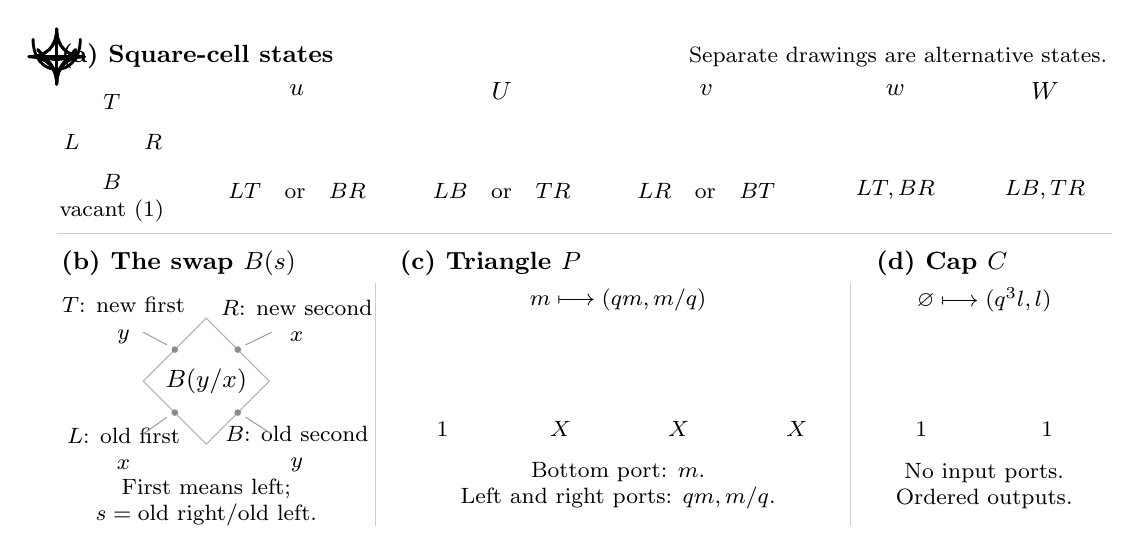
\begin{tikzpicture}[
  x=1cm,y=1cm,
  font=\small,
  finite boundary/.style={draw=black!30,line width=.4pt},
  finite arc/.style={draw=black,line width=1.05pt,line cap=round},
  every node/.style={inner sep=1.5pt},
  finite label/.style={font=\footnotesize},
  finite heading/.style={anchor=west,font=\small\bfseries}
]
  \node[finite heading] at (0,0) {(a) Square-cell states};
  \node[anchor=east,font=\footnotesize] at (13.4,0)
    {Separate drawings are alternative states.};

  \FiniteSquare{.70}{-1.08}{}
  \node[finite label,left]  at (.35,-1.08) {$L$};
  \node[finite label,below] at (.70,-1.43) {$B$};
  \node[finite label,right] at (1.05,-1.08) {$R$};
  \node[finite label,above] at (.70,-.73) {$T$};
  \node[finite label] at (.70,-1.96) {vacant ($1$)};

  \node at (3.05,-.43) {$u$};
  \FiniteSquare{2.50}{-1.08}{%
    \draw[finite arc] (-.35,0) .. controls (-.13,0) and (0,.13) .. (0,.35);}
  \FiniteSquare{3.60}{-1.08}{%
    \draw[finite arc] (0,-.35) .. controls (0,-.13) and (.13,0) .. (.35,0);}
  \node[finite label] at (3.05,-1.70) {$LT\quad\text{or}\quad BR$};

  \node at (5.65,-.43) {$U$};
  \FiniteSquare{5.10}{-1.08}{%
    \draw[finite arc] (-.35,0) .. controls (-.13,0) and (0,-.13) .. (0,-.35);}
  \FiniteSquare{6.20}{-1.08}{%
    \draw[finite arc] (0,.35) .. controls (0,.13) and (.13,0) .. (.35,0);}
  \node[finite label] at (5.65,-1.70) {$LB\quad\text{or}\quad TR$};

  \node at (8.25,-.43) {$v$};
  \FiniteSquare{7.70}{-1.08}{\draw[finite arc] (-.35,0)--(.35,0);}
  \FiniteSquare{8.80}{-1.08}{\draw[finite arc] (0,-.35)--(0,.35);}
  \node[finite label] at (8.25,-1.70) {$LR\quad\text{or}\quad BT$};

  \node at (10.65,-.43) {$w$};
  \FiniteSquare{10.65}{-1.08}{%
    \draw[finite arc] (-.35,0) .. controls (-.13,0) and (0,.13) .. (0,.35);
    \draw[finite arc] (0,-.35) .. controls (0,-.13) and (.13,0) .. (.35,0);}
  \node[finite label] at (10.65,-1.70) {$LT,BR$};

  \node at (12.55,-.43) {$W$};
  \FiniteSquare{12.55}{-1.08}{%
    \draw[finite arc] (-.35,0) .. controls (-.13,0) and (0,-.13) .. (0,-.35);
    \draw[finite arc] (0,.35) .. controls (0,.13) and (.13,0) .. (.35,0);}
  \node[finite label] at (12.55,-1.70) {$LB,TR$};

  \draw[black!20] (0,-2.25)--(13.4,-2.25);
  \node[finite heading] at (0,-2.62) {(b) The swap $B(s)$};
  \node[finite heading] at (4.30,-2.62) {(c) Triangle $P$};
  \node[finite heading] at (10.35,-2.62) {(d) Cap $C$};

  \draw[finite boundary] (1.90,-3.32)--(2.70,-4.12)--(1.90,-4.92)--(1.10,-4.12)--cycle;
  \node at (1.90,-4.12) {$B(y/x)$};
  \foreach \p in {(1.50,-3.72),(2.30,-3.72),(1.50,-4.52),(2.30,-4.52)}
    \fill[black!45] \p circle (1.2pt);
  \node[finite label,align=center] at (.85,-3.35) {$T$: new first\\$y$};
  \node[finite label,align=center] at (3.05,-3.35) {$R$: new second\\$x$};
  \node[finite label,align=center] at (.85,-4.98) {$L$: old first\\$x$};
  \node[finite label,align=center] at (3.05,-4.98) {$B$: old second\\$y$};
  \draw[black!40,line width=.35pt] (1.40,-3.66)--(1.10,-3.50);
  \draw[black!40,line width=.35pt] (2.40,-3.66)--(2.73,-3.50);
  \draw[black!40,line width=.35pt] (1.40,-4.58)--(1.10,-4.79);
  \draw[black!40,line width=.35pt] (2.40,-4.58)--(2.73,-4.79);
  \node[finite label,align=center] at (1.90,-5.66)
    {First means left;\\$s=\text{old right}/\text{old left}$.};

  \draw[black!20] (4.05,-2.88)--(4.05,-5.96);
  \node[finite label] at (7.13,-3.09) {$m\longmapsto(qm,m/q)$};
  \FiniteTriangle{4.90}{-4.06}{}
  \FiniteTriangle{6.40}{-4.06}{%
    \draw[finite arc] (0,-.33) .. controls (0,-.14) and (-.09,-.07) .. (-.24,.09);}
  \FiniteTriangle{7.90}{-4.06}{%
    \draw[finite arc] (0,-.33) .. controls (0,-.14) and (.09,-.07) .. (.24,.09);}
  \FiniteTriangle{9.40}{-4.06}{%
    \draw[finite arc] (-.24,.09) .. controls (-.13,-.08) and (.13,-.08) .. (.24,.09);}
  \node[finite label] at (4.90,-4.73) {$1$};
  \node[finite label] at (6.40,-4.73) {$X$};
  \node[finite label] at (7.90,-4.73) {$X$};
  \node[finite label] at (9.40,-4.73) {$X$};
  \node[finite label,align=center] at (7.13,-5.45)
    {Bottom port: $m$.\\Left and right ports: $qm,m/q$.};

  \draw[black!20] (10.08,-2.88)--(10.08,-5.96);
  \node[finite label] at (11.78,-3.09) {$\varnothing\longmapsto(q^3l,l)$};
  \FiniteCap{10.98}{-4.06}{}
  \FiniteCap{12.58}{-4.06}{%
    \draw[finite arc] (-.30,.22) .. controls (-.30,-.29) and (.30,-.29) .. (.30,.22);}
  \node[finite label] at (10.98,-4.73) {$1$};
  \node[finite label] at (12.58,-4.73) {$1$};
  \node[finite label,align=center] at (11.78,-5.45)
    {No input ports.\\Ordered outputs.};
\end{tikzpicture}
\endgroup
\caption{Local states and port conventions. Gray outlines locate the cells
and gray dots locate possible ports; only black curves denote occupied
arcs. The two curves in a $w$- or $W$-state occur together. Panel~(b)
records the port interpretation of the same square, rotated so that old
ports are below new ports; it does not select a matching. Each drawing in
panels~(c) and~(d) is one allowed state, with its weight underneath.
Transposition reverses inputs and outputs.}
\label{L:fig:local-states}
\end{figure}


Here is a verification. A square root is continued multiplicatively in each identity (using \(q^{1/2}=e^{\pi i/8}\)); different choices just conjugate on occupied ports since only the single corners change sign. For inversion \(B(s)B(s^{-1})=1\), write \((a,b,c,d,e)\), \((A,B',C',D',E)\) for weights \((u,U,v,w,W)\) of the two factors from bottom to top. The matching coefficients use
\(B'+D'b=b+B'd=A c+C'a=B'b+D'e+E d=0\), \(A a+C'c=D'd=1\).
A quarter turn changes \(s\) to \(q^3/s\). Thus bending a leg in inversion gives cap sliding, e.g. \(B_{23}(s)B_{12}(q^3s)(1\otimes C)=C\otimes1\).
For triangle sliding the transpose version is
\[
 (P^t\otimes1)B_{23}(qs) B_{12}(s/q)=B(s)(1\otimes P^t).
\]
For clarity the scalar check below labels exterior ports \(0,1,2,3,4\) (inputs \(0,1,2\), outputs \(3\) right and \(4\) left); juxtaposed pairs mean both arcs. Now lower-case \(a,\ldots,e\) denote weights at \(s/q\); write capital \(A,B,C,D,E\) at \(qs\) just in this table. Entries of the two sides (with the empty coefficient 1 omitted) are the equal expressions
\[
\begin{array}{c|l|l@{\qquad}c|l|l}
23&A+EXb&Xu&12&Ba+C Xc&X\\
13&B Xc+C a&Xu&01&A Xd+b&XU\\
02&B c+C Xa&XU&03&B Xa+C c&v\\
34&B X+C Xb&U&24&B Xb+C X&Xv\\
14&A Xa+X c&Xv&04&A Xc+X a&u\\
01,23&A b+D Xd+E Xe&0&14,23&A Xc+D Xa&0\\
12,34&E Xa&XU&01,34&B Xb+C Xe&XW\\
01,24&B Xe+C Xb&0&02,34&E Xc&XW\\
04,23&A Xa+D Xc&Xw&04,12&B Xd&Xu\\
04,13&C Xd&Xw&03,12&E Xd&Xv
\end{array}
\]
Here entries on the left of each equality just split by the connections at the triangle (closed loops dropped). These scalar equalities and the inversion coefficients follow by substitution; e.g. use \([n]=\sin(\eta+n\pi/8)\) and substitute
\((\sin(10\pi/8)[5],\sin(10\pi/8)[0],-[5][0],[5][-2],-[-1][0])/([10][3])\), shifting brackets by \(\pm1\) for upper/lower-case, and \([n][j]=(\cos((n-j)\pi/8)-\cos(2\eta+(n+j)\pi/8))/2\).
Transpose and reflection give, in particular, \(B_{23}(s/q)B_{12}(qs)(1\otimes P)=(P\otimes1)B(s)\). Finally
\(B_{12}(s)B_{23}(sr)B_{12}(r)=B_{23}(r)B_{12}(sr)B_{23}(s)\):
as functions of \(r\) clear the four linear pole factors from \(B(r),B(sr)\) (a cell has poles only at arguments \(q^5,q^6\), and bounded weights at 0 and \(\infty\)); matching coefficients have degree \(\le4\) and powers integer, or all half-integer between 0 and 4 by port parity (a square-root flip on a rapidity multiplies by \(-1\) per occupied end carrying it). Check \(r=1,q^2,q^3\) by identity or triangle/cap sliding of both halves of \(B(r)\) across the third strand. Check \(rs=q^2,q^3\) the same way (move the invertible \(B(s)\)'s across the equality). This proves the braid relation by interpolation. All these relations apply to a row and carry through closure with seam twist. Swaps on spatial neighbors intertwine row addition; on a cylinder moving the seam past a position conjugates by the sign \(\sigma\) on that occupied position (even parity at each cell). Carrying it past a whole pattern gives no sign.

\subsection{Polynomial denominators}\label{L:step2}

Both \(A_\delta=Q\) for \(\delta=1\) and \(A_\delta=R\) for \(\delta=2\) are symmetric polynomials of degree \(\le\delta(N-1)\) per variable: poles at coincident points cancel by equal rows (twice for the symmetric determinant), and cell-kernel denominators cancel from \(F^\delta\). Their recursions are
\begin{equation}\label{L:eq:polynomial-reductions}
\begin{array}{l|l|l}
 &Q&R\\ \hline
 (l,q^3 l,Z)/ (Z) &(1+q^3)l\prod d(z,l)
 &\kappa^2[(1+q^3)l\prod d(z,l)]^2\\
 (qm,m/q,Z)/(m,Z)&\sqrt2\,m\prod(z+m)&k\sqrt2\,m^2\prod(z+m)^2\\
 (0,Z)/(Z)&\prod z &\prod z^2
\end{array}
\end{equation}
At infinity the leading coefficient is the smaller polynomial. The first line is pole-pair elimination. To check the second put \(f_m(s)=(m^4+s^4)/(m^4-s^4)\), \(A(s,t)=(s^2-t^2)/h(s,t)\). The Schur complement kernel after pivoting on \((b,c)=(q m,m/q)\), by substitution, is
\[
 \begin{aligned}
 &A(s,t)+[A(s,c)A(t,b)-A(s,b)A(t,c)]/A(b,c)\\
 &\qquad=f_m(s)f_m(t)[A(s,t)-A(s,m)+A(t,m)]
 \end{aligned}
\]
with the extra column becoming \(-f_m(s) A(s,m)\); for \(M\) the complement is \(f_m(s) f_m(t)[M(s,t)-M(s,m)M(m,t)]\). The skew brackets give the smaller Pfaffian including \(m\) (eliminate its pairing with the augmenting column, or if using the transformed extra column turn it into \(m\) by row/column additions). Meanwhile \(F\) contributes \(h(b,c)/(b-c)\prod(z+m)/f_m(z)\) relative to the fused set. These identities give the table. At \(0,\infty\) the row of \(M\) just decouples; for the Pfaffian the row supplies the column augmentation or eliminates it. Inversion of all variables transforms \(A_\delta\) by the monomial factor \(\prod z^{-\delta(N-1)}\).

\begin{proposition}[Polynomial half-cylinder vectors]\label{L:prop:vacuum-polynomials}
For each pairing pattern $p$ and seam sign $\sigma\in\{+1,-1\}$, the
normalized physical vacuum has the form
\[
 (V^\sigma_N)_p(Z;t)
    = \frac{\prod_j z_j^{o_j/2}}{A_\delta(Z)}\,\psi_{p}(Z),
 \qquad \deg_{z_j}\psi_p\le\delta(N-1)-o_j ,
 \qquad
 \delta=\begin{cases}1&\sigma=1,\\2&\sigma=-1,\end{cases}
\]
independent of the row parameter. Here \(o_j=1\) for an occupied port of pattern \(p\), 0 otherwise. At adjacent high-then-low pairs of rapidities \(q^a l,l\) the vector is \(P V^\sigma_{N-1}\) (fused rapidity \(q l\)) for \(a=2\) and \(C V^\sigma_{N-2}\) for \(a=3\), if the seam is not between the two. Branches at a specialization use \((q^a l)^{1/2}=q^{a/2}l^{1/2}\); thus this prescribes values of the branch-independent polynomials \(\psi\). The same parity convention holds under all transports. At a variable 0 or infinity the normalized vector \(V\) with that port vacant goes to the vector with position dropped, and occupied components vanish there. There is covariance under nearest rapidity exchanges (by \(B\), away from the seam) and cyclic rotations (moving the seam with the conjugating sign above), thus also rules across the seam by first rotating.

\end{proposition}
\begin{proof}
We induct on the number of columns. The induction constructs a polynomial
vector from smaller vacua; only after proving its row invariance do we
identify it with the convergent physical vacuum. At each smaller size the
induction hypothesis includes the degree and removal rules, pair reductions,
and exchange and cyclic covariance in the statement.

For startup \(N=0,1\) there is just the vacuum; for \(N=2\) use normalized empty value 1 and the single pair value
\[
 \frac{\sqrt2 X\sqrt{z_1 z_2}}{z_1+z_2}
 \quad\text{or}\quad
 \frac{2\kappa X}{q-q^{-1}}\,
 \frac{(z_1-z_2)\sqrt{z_1 z_2}}{z_1^2+z_2^2+2\kappa z_1z_2}
\]
in the two sectors (product square roots). These obey the degrees, both orientations of pair prescriptions (value \(X\) or 1 in seam-avoiding high-left order, with rotation sign), and removals. Row invariance follows by sliding at the four nodes and degree (the empty component is immediate). At these sizes, uniqueness near the physical point identifies the vectors and gives exchange and cyclic covariance by the row intertwining relations.

\paragraph{Prescribing values from smaller vacua.}
Fix $N\ge3$. Our first task is to define polynomial data on the pair
hyperplanes and prove that different prescriptions agree where they meet.
Write \(S_{hl}^a\) for the \emph{proposed polynomial value} on \(z_h=q^a z_l\), given by the adjacent triangle/cap rule just stated from the smaller solution and rescaled by \(A_\delta/\prod z_j^{o_j/2}\). For nonadjacent \(h,l\), take the ordered cyclic arc from \(h\) to \(l\) along increasing indices. Bring the partners together across intervening positions (to some slot in these, whose own order is kept), use the adjacent rule and transport the vectors \textbf{before the diagonal rescaling} back via neighbor swaps. In the linear, nonwrapping case one need not move the seam; for a wrapping arc rotate using the sign convention to avoid it.

The definition is independent of the slot, and covariant before rescaling under swapping neighbors other than swapping the two partners through each other. Indeed moving an intervening position from one side of the slot to the other is precisely sliding the triangle/cap (and exchanging with the fused rapidity in the smaller solution); use also inversion on the exchanges with individual partner lines. Thus a further swap involving one partner just extends or undoes one of the transport moves (take the slot at the other end of the arc); a swap of two spectator positions commutes through the transports by braid to the smaller solution. These arguments can be done first with all other rapidities generic. Rotation with the sign convention is consistent here: crossing the seam with a block at a slot gives the same twist on the two outputs of a triangle together as on its input, and no twist for both outputs of a cap. Equivalently use the conjugated swap for a move across the current cut. This uses covariance of the smaller solution under exchanges and rotations. Thus for the cyclic prescriptions one can rearrange positions along the circle, using these covariances at each neighboring exchange not of \(h,l\) with each other.

Each such value is polynomial, in particular of degree \(\le\delta(N-1)-o_j\) in any spectator. To see regularity, cancel the smaller denominator first using the \(A_\delta\)-table. For an intervening position \(s\), moving \(l\) back to the right creates possible poles at \(z_s/z_l=q^5,q^6\); moving \(h\) left instead gives \(q^{a+2},q^{a+3}\). The only common pole locations are killed by the factors \((z_s+q z_l)^\delta\) or \(d(z_s,z_l)^\delta\) in the two respective reduction ratios (\(a=2,3\)); swaps there have at most simple poles generically along each divisor. All expressions after rescaling have integral powers (flipping a square root, or the common square root of a pair and its fused variable, only gauges occupied legs). 

At a spectator extreme the smaller normalized vector and all swaps are bounded at generic other values, giving regularity and the degree by parity. More precisely with the spectator vacant the normalized value goes to the same prescription with spectator dropped: corners involving it singly go to zero, opposite-side weight tends to 1. If the two partners tend together to 0 (respectively infinity), normalized vectors again are bounded, and before division by the half power monomials their rescaling by \(A_\delta\) has order \(O(z_l^\delta)\) (respectively \(O(z_l^{\delta(2N-3)})\)), by the reduction table. This also rules out poles at the pair origin.

\paragraph{Compatibility of the prescribed values.}
The preceding argument concerns one pair hyperplane at a time. Coordinate
interpolation will also require agreement when two such hyperplanes meet;
this is the remaining property of the data to establish before constructing
the size-$N$ vector. We record that compatibility next. In the case \(\delta=1\) we only intersect \emph{linear high-before-low} prescriptions (\(h<l\)); for \(\delta=2\) we allow cyclic ones. At generic points of the intersection of constraints on two different unordered pairs, \(S\) gives the same polynomial value by either prescription.
\begin{itemize}
\item For disjoint pairs, use regular swaps and covariance to make both consecutive forward. This can be done preserving the two orientations (linearly by reordering subject to the two constraints; cyclically by shrinking each of the two ordered arcs independently, letting its members pass through other positions but not each other). More formally one may move points continuously on a circle and record regular adjacent transpositions; for each disjoint pair keep the oriented spacing strictly between 0 and one full circumference and end with the pairs in disjoint tiny intervals. Then reductions commute by induction.
\item With a shared high or shared low site, the two other sites differ by zero or one power of \(q\), so are freely exchangeable. Move the three to a consecutive triple sorted by the exponents using regular swaps not crossing either constrained pair (and a rotation if necessary). On the circle the other two sites can be placed to the desired side of their fixed common site without passing it. Equal exponents give identity swap and compatibility. Otherwise the exponents modulo a common shift are \(3,1,0\) or \(3,2,0\). Fusing the pair at gap two and then the resulting gap two is the same as taking the cap at gap three and swapping the intermediate site back into place: \((P\otimes1)P=B_{23}(q)(C\otimes1)\), or the reflected identity. This is two triangles making a cell \(B(q)\) (weights \(X,X^2,X^2,X^2,0\)); the cap simply continues its adjacent leg or leaves it vacant.
\item With consecutive gaps sharing the middle of a chain of two directed constraints, gaps \(2,2\) allow sorting into the triple \(4,2,0\) as above (gap four is freely exchangeable). Either reduction is fusion and then cap, yielding weight 1 on the empty local output and \(X\) on each possible cup. The other cases give a wheel (three cyclic exponent gaps \(2,3,3\) in some order); both polynomial values vanish by \((z_s+qz_l)^\delta\) or \(d(z_s,z_l)^\delta\) in the ratios, the lower polynomials regular. For linear constraints the third site need not be crossed when bringing partners together. For cyclic constraints it might be crossed once with a simple pole but then \(\delta=2\).
\end{itemize}
All transports in these checks can be applied also to the \(A_\delta V\) vectors themselves so do not require dividing by an intersection zero. Branch signs in nonzero checks can be chosen coherently along the two constraints. For linear constraints all the reorderings can preserve the partner orders.

\paragraph{Constructing one polynomial vector.}
For each distinguished \(i\), form a chart by polynomial interpolation in \(z_i\) at these nodes: for \(\delta=2\) both \(z_i=q^{2,3}z_j\) for every \(j\ne i\) (\(i\) always high), and for \(\delta=1\) only \(q^3z_j\) if \(i<j\), \(q^{-3}z_j\) otherwise, using \(S\). In both cases add the node 0 when \(o_i=0\), with polynomial value \(\prod_{j\ne i}z_j^\delta\) times the lower polynomial. 

These charts are polynomials in all variables: any nonzero node coincidence divisor between two positions gives only simple poles (even if there are two coincidences, they are at different nodes), canceled by the compatibility just proved. At \(z_j=0\), the \(\delta\) colliding moving nodes have values of order at least \(\delta-(o_i+o_j)/2\) (rounded up), by the pair-origin estimate; the origin value itself if used has a factor \(z_j^\delta\), so no term has a pole. 

At \(z_j=\infty\), moving nodes from \(j\) have values of order \(O(z_j^{\delta(2N-3)-(o_i+o_j)/2})\) and their Lagrange factors cost a power at most \(\delta-1-[\delta(N-1)-o_i]\). Thus all terms obey the degree bound in \(j\), and these moving-node terms do not contribute to its highest power when \(o_j=0\). In that case the leading coefficient of the other terms together is exactly the lower polynomial (on dropping \(j\)): values go to the reduced prescriptions and the bounded-node basis factors to the smaller interpolation basis, using the vacant-spectator limit above.

Chart \(i\) satisfies the same pair prescriptions on \emph{other} pairs (\(i\notin\{h,l\}\); just the gap-three linear constraints for \(\delta=1\)). Indeed on specializing there, check at its defining nodes in \(z_i\): no coincidences forced, compatibility applies, and the vacant 0-value also works by spectator removal. The degree bound proves equality. 

Thus for two charts \(i,j\), take a third site \(k_0\): they agree on both sets of constraints with \(k_0\) low in the \(\delta=2\) case (one or other exponent \(2,3\), all partners), or the annular gap-three constraints in fixed linear order with \(k_0\) in either role for \(\delta=1\). These are \(\delta(N-1)\) nodes in \(z_{k_0}\); if that position is vacant the leading coefficient also agrees by the preceding infinity argument. Hence all charts coincide (\(N\ge3\)). In particular both extreme-value rules hold. For \(\delta=1\) this common polynomial also satisfies the gap-\emph{two} linear prescriptions: compare to \(S_{hl}^2\), \(h<l\), at the nodes of a third site's chart by the same compatibility and degree. The two moving nodes from \(h,l\) cannot collide on this specialization even if the site lies between them (\(q^{-3}q^2\ne q^3\)).

The charts now define one family of component polynomials $\psi_p$.
Undo the diagonal normalization and write
\[
 (\widehat V_N^\sigma)_p
 =\frac{\prod_j z_j^{o_j/2}}{A_\delta(Z)}\,\psi_p(Z).
\]
We have proved the degree bounds, both extreme-value rules, and the
available ordered pair reductions for $\widehat V_N^\sigma$. Row invariance and identification with the size-$N$ physical vacuum remain
to be proved.
The empty polynomial component is \(\psi_\emptyset=A_\delta\), hence \((\widehat V_N^\sigma)_\emptyset=1\): transports and reductions have normalized empty value 1, since any extra closed cycle is killed.

\paragraph{Row invariance and physical identification.}
We next prove $T_\sigma\widehat V_N^\sigma=\widehat V_N^\sigma$ by testing
the residual at the pair prescriptions. Indeed this is true at all the available ordered pair prescriptions by sliding triangle/cap and swaps and using induction on the smaller row. Multiply the difference by \(A_\delta\), clear the single row-cell denominator \(d(z_i,t)\) in a variable and divide by \(z_i^{o_i/2}\); this gives a polynomial of degree at most \(\delta(N-1)+2-o_i\), by boundedness at endpoints, port parity and the chart result. For \(\delta=2\) there are \(4(N-1)\) nodes, and for \(\delta=1\) at least \(2(N-1)\); these suffice for \(N\ge3\), with the extra check at 0 by vacant-port reduction (the empty spatial port propagates the auxiliary one by \(v\to1\) or vacancy) if \(N=3,\delta=1,o_i=0\). The same argument works if another seam position is needed in making reductions, by row rotation with port sign conjugation.

Uniqueness for the row near the physical point now gives
$\widehat V_N^\sigma=V_N^\sigma$. Braid intertwining supplies exchange
covariance, and moving the seam supplies cyclic covariance. Consequently
the available high-left reductions extend by cyclic transport, completing
all parts of the induction hypothesis at size $N$.
\end{proof}


\subsection{Gluing rules}\label{L:step3}

Glue a lower and an upper vacuum through the marked row opened at the seam, asking for both open ends occupied and connected, no other loops. Upper vacua are given by up/down reflection (\(s\mapsto q^3/s\), i.e. take spatial rapidities \(z_j^{-1}\) and row parameter \(1/(q^3t)\)); in particular the same \(A_\delta(Z)\) up to monomials serves as denominator, and they, like the lower vacua, are independent of \(t\). Matchings alone suffice in this gluing. For \(E_+\) take both vacua with positive twist. For \(J\) take \(\sigma=-1\) below and \(+1\) above, without any extra factor at the mark.

Here is why the mixed gluing works. Orient each rooted loop in the direction from last to first column at the mark (positive seam crossing), and temporarily multiply its weight by
\[
 -i\exp(i\,{\rm turn}/4+i\pi h_0/2),
\]
where \(h_0\) is the signed total seam crossing number. For this argument use a flat square-cell cylinder with simple curves normal to and smooth across crossed sides. A simple winding loop has \(h_0=\pm1\), turn 0, and a contractible one has \(h_0=0\), turn \(\pm2\pi\). Indeed on the twice-punctured sphere successive crossings met along the seam alternate signs by separation. In the zero-translation case we can lift the loop to a planar simple closed curve; in the other case lift arbitrarily many periods starting at a highest point of the loop and close above, using simplicity and bounded added turn to get zero turn per period. The displayed factor changes sign on reversal, and in the winding case equals \(h_0\); summing it over the marked crossings of a given orbit under row translations thus gives 1 if winding and 0 otherwise. Rearrangement here is absolutely convergent.

For a fixed matched diagram in a half-cylinder we can represent its pairing canonically without crossing the seam (noncrossing along the ordered boundary). Replacing both half diagrams so, keeping the opened row, the factor is 1 (only the mark crosses). For a pair \(i<j\) below the row, traversed from \(i\) to \(j\), the actual lift has horizontal index displacement \(j-i\) or \(j-i-N\); any further shift would interlace a translate, impossible. Its contribution to turn, from incoming to outgoing normal, is \(+\pi\) or \(-\pi\) respectively (close along the boundary), and to seam number 0 or \(-1\). Thus the factor relative to canonical is \(1\) or \(-1\), exactly the lower seam twist, also for reversed traversal. Above the row the turn signs switch and the relative factor is always 1. This proves the mixed rule.

Consequently these sums are symmetric in \(Z\), obey both removal rules and both pair recursions without multipliers (just reducing to the same quantity at fused/remaining rapidities), and have a polynomial numerator on multiplying by \(A_{\delta_{\rm below}} A_{\delta_{\rm above}}\prod d(z,t)\) of degree at most \((\delta_{\rm below}+\delta_{\rm above})(N-1)+2\) per variable \(z_i\). Indeed all neighbor exchanges within the linear sequence of columns and the reduction surgery there avoid the opened seam, so cycles closed off during manipulations can always be killed. For a high-then-low adjacent reduction, slide \(P\) or \(C\) from below to above. It contracts there to the smaller vacuum: on the reversed rapidity relation above, exchange of the pair uses \(PP^t\) or \(CC^t\), while the exchanged vacuum is \(P\) or \(C\) times the smaller one. The maps \(P,C\) are injective on pairing states (read off components with both new sites vacant or with a single prescribed one occupied). Branches for reflected cells are obtained by angle complementation. The same slide with an ordinary invertible swap proves symmetry using the two vacuum exchange relations (upper exchange by the inverse): \(B(s)^t=B(s)\) on diagrams (reflection exchanging \(L,T\) and \(B,R\)), and upper rapidity ratios are the reciprocals of lower ones. Thus a swap left over at the upper boundary after interchanging two adjacent columns is absorbed by upper exchange covariance. Only adjacencies not across the mark are needed for this symmetry. At a variable extreme both vacua decouple on an empty port, and the horizontal-only propagation at that cell has limiting weight 1. Polynomiality and bounds follow from the vacuum bounds, the cell denominators and square-root parity. Formally at zero size \(E_+=J=1\) (straight auxiliary identity).

There is also a mark constraint. Take the marked first column of parameter \(x\): at \(t=x\) the mark port is tied to \(T\) there if either is occupied, at \(t=x/q^3\) to \(B\). Thus in the closed-row picture we can equivalently require a single loop through that slice port. Propagating the lower or upper state respectively through the row by invariance now reduces to gluing both vacua at a slice (with that one-cycle, first-port-occupied condition); cycles closed off within the propagated half cannot be the target loop so are correctly killed. One just corrects for the twist factor now included at the mark by the propagated row. Thus \(E_+\) at both parameters equals that pure slice gluing of positive vacua, and \(J(t=x)=-J(t=x/q^3)\) (negative twist from below only). Symmetry gives the analogous row-parameter constraints for any \(x\in Z\). In particular \(E_+(Z;t=x)\) for \(x=z_1\) gives the actual polygon mass through a first column top port in the honeycomb evaluation of the vacua, where applicable (in particular at regular homogeneity).

Now formula~\eqref{L:eq:one-port} for \(E_+\) has the stated degree, both pair recursions by the \(Q\)-table, and both removal values. This suffices for uniqueness when \(N\ge2\); at \(N=1\) add the evaluation \(t=x\) (value 0 on both sides). For \(YJ\), \(Y\) preserves pair recursions and multiplies removal values by \(\kappa\); allow denominator \(R^2\prod d\) and degree \(4(N-1)+2\) throughout. The proposed wave formula satisfies the pair recursions: the joint projection residual kernel of \(M\) transforms by \(f_m(s)f_m(u)\) relative to the fused value by the Schur identity, or trivially under removal of a pole pair \(l,q^3 l\) by Schur elimination. Reading the first orders as the external variable \(u\to\infty,0\) gives \(-f_m(s)p^+(s)\), \(+f_m(s)p^-(s)\) relative to the fused waves, and \(f_m(q^3t)=1/f_m(t)\). Removing instead a position by sending it to infinity multiplies \(p^+\) by \(1-k\) and preserves \(p^-\) (one more Schur complement, using \(M(s,u)\sim k s/u\)); at 0 their roles interchange. Thus \(YJ\)'s proposed expression has the right removal values. It obeys the denominator and degree bounds: each projection has denominator cleared by \(R\) and external factors \(h(s,z)\), by the bordered determinant (poles of \(F^2\) there cancel as for \(R\)). In a wave product unwanted poles in \(z\) at \(t,q^3t\) cancel because the partner wave vanishes at a generic interpolation node \(s=z\). Bounds at the extremes then suffice. At \(t=x\) the zero is multiplied by a pole at \(q^3t=q^3x\); at \(t=x/q^3\) by a pole on the opposite shift. The coefficients of these two poles in multiplicative coordinates are opposite (the row \(M(s,Z)\) is the only source, \(M(s,x)=M(x,s)\)); pairing the summands by symmetry of the two-wave expression gives the negative-value constraint exactly.

For later use the marked-row evaluations just proved may be recorded as
\begin{equation}\label{L:eq:mark-evaluation}
 E_+(Z;x)=E_+(Z;x/q^3),\qquad J(Z;x)=-J(Z;x/q^3)
 \quad(x\in Z),
\end{equation}
with the common first value given by the occupied-port slice gluing.

More explicitly, on induction all pair nodes and 0 and infinity match, so the remaining ambiguity for \(YJ\) is only a scalar multiple of
\[
 \mathcal W_N(Z;t)=\frac{\prod_{i<j}K(z_i,z_j)}{R(Z)^2}
                     \prod_i \frac{z_i t}{d(z_i,t)}.
\]
This follows by divisibility and degree variable by variable and common scaling invariance. Its two shifted values do not sum to zero identically (the single marked-site factors agree and are nonzero, while for each other independent variable the ratio of the two factors is nonconstant). Thus the constraint proves equality starting with the displayed zero-size value.

Finally consider the color sum, with normalization
\[
 L(Z)=R(Z)^2/\prod_{i<j}K(z_i,z_j),\qquad O_Z(r)=L(Z)^{-1}\sum_\alpha\prod_i b_{\alpha_i}\prod_{i<j}P_{\alpha_i\alpha_j}(z_j/z_i).
\]
It is symmetric. For a pair \(x,y\) (labels in that order), in the raw sum:
\begin{itemize}
\item At \(y=q^2x\) the contributing residue labels fuse as \(+0\mapsto+\), \(0-\mapsto-\), \(+-\mapsto0\) at \(qx\). At \(y=q^3x\) only \(+-\) contributes, going to vacant.
\item The simple extraneous pole at \(y=qx\) cancels between \(+-\) and \(00\); at \(y=x\) all simple poles cancel by symmetry.
\end{itemize}

To verify residues, the pair factors involving a spectator \(u\) in the first rules multiply to the reduced ones times \(S(u/(qx))\) (fusion), or times \(S(u/(qx))S(u/(q^2x))\) (gap three), precisely the relative spectator factors of \(L\) by the table. For the canceling pole the spectator products agree. These identities follow immediately by inserting the entries of \(P_{ab}\). With coordinate \(y/y_0-1\), let \(D_0=k/(q-q^{-1})\) be the pole coefficient of \(S\) at \(q\). The remaining pair multiplier (for the residue relative to the reduced term) for each fusion choice is \(k D_0\) (use \(S(1)=2k\)), and for gap three \((k/2)S(q^2)D_0\). These are exactly the relative pair pole coefficients of \(L\): use \(K(1,y/x)\)'s linear coefficients \(-2i\sqrt2,-2\) at the two positive gaps in these coordinates, and the \(R\)-ratios above. At \(qx\) the two coefficients are \(-b_+b_- S(1)D_0,\ b_0^2D_0\). Symmetry covers the reversed locations.

Hence \(O_Z(r)\) obeys both pair recursions with no multipliers, and \(R(Z)^2 O_Z(r)\) is polynomial of degree \(\le4(N-1)\) per variable (all factors bounded at extremes). Removal at 0 or infinity multiplies \(O\) by \(r\) since all added pair factors tend to 1 and \(L\) drops to the smaller value. The pair recursions with a single endpoint value thus determine it uniquely at all sizes from \(O_\emptyset(r)=1\). For the three choices of \(r\) the claimed powers of \(Y\) satisfy the same checks by the denominator table, as required.


\section{Change of expansion for the color sums}\label{L:part2}

The purpose of this section is to represent the finite color sums of
Section~\ref{L:part1} by a convergent Gaussian expansion on a circle.
Proposition~\ref{L:prop:scalar-channel} gives the scalar change of channel
for a fixed list of charges; Section~\ref{L:step5} then recovers the raw
finite sum exactly by a constant coefficient. This representation is the
input to the long-circle estimate in Section~\ref{L:part3}. We first set up
the charge space and justify the formal trace operations, then prove the
scalar identity, and finally establish the stability and convergence
needed to sum over all root insertions.

Use the conjugate convention \(q\mapsto q^{-1}\) in the preceding factors \(P_{ab}\), and write
\[
 b_+=w=\sqrt{k/2}\,e^{i\phi},\qquad b_-=\bar w,\qquad b_0=k .
\]
We use \(\phi=-7\pi/8,-\pi/8\), giving \(r=1,\kappa^2\) respectively. By a raw sum we mean without the multiplier \(\prod K/R^2\); the variables of interest are \(Z=1^N\).

\subsection{Charge space and the formal trace}

Use real vectors \(D_j\), \(j\bmod8\), with one relation \(\sum D_j=0\); take the symmetric bilinear product
\[
 D_0 D_j=(2,-1,1,-2,2,-2,1,-1)_j,\qquad O D_j=D_{j+1}
\]
translated cyclically. It is nondegenerate on this quotient (e.g. cyclic Fourier transform), but not positive. Define \(a\) by \((1-O+O^2)a=D_0\); its row \(aD_j\) is \((1,0,0,-2,0,0,1,0)\). Put \(\Lambda=\sum\mathbb Z D_j,\ S=(1-O)^{-1}\). The color vectors are
\[
 a,\quad a-D_0=(O-O^2)a,\quad a-D_0-D_1=-O^3a ,
\]
all of square \(8/3\). Further put
\[
 \delta=D_7,\quad R_\delta y=y-\delta(\delta y),\quad M_b=O R_\delta,\quad h=-OS\delta=-S D_0,\quad H_b=h^2=9/8 .
\]
The rows \(hD_j=(-1,0,-1,1,-1,1,0,1),\ Sa\cdot D_j=(1,1,1,-1,-1,-1,0,0)\). We have \(S+S^t=1\) (metric transpose), \(S\Lambda\cdot\Lambda\subset\mathbb Z\), \(M_b h=h,\ \delta h=1,\ ah=0\), and
\[
 \det(I-yM_b)=(1-y^6)(1-y^3)/(1-y^2)
\]
on the quotient. These follow by multiplication (one can use \(S=-\sum_{j=0}^7 j O^j/8\)); for the determinant multiply \(\det(I-yO)\) by \(1+\sum_{n\ge1}y^n\delta O^n\delta\) by the rank-one change. In particular the fixed axis of \(M_b\) splits off.

Use parameters, initially \(L>0\),
\[
 p=e^{-L/8},\qquad \mathfrak q=e^{-4\pi^2/L},\qquad s=e^{-2\pi i u/L},\qquad u=x+2\pi i d
\]
with angles \(d\) in an open interval of length 1 about 0. Operators in products act in order of increasing \(d\). The sources (variables \(z=e^{u/8}\)) near 1 have angles close to 0.

The coefficient algebra uses the lattice fields and root-mode relations of vertex-operator constructions \cite[Section~2.1, equations~(2.2)--(2.5)]{Frenkel1985}. We give the formulas and verify their use in this indefinite bilinear space, where convergence is a separate issue. At momentum \(P\), take polynomials freely generated from \(|P\rangle\) by oscillators \(l_{-m}(y)\), \(m>0\), linear in a vector \(y\) in the above space (complexified); let
\([l_n(y),l_m(z)]=n\mathbf1_{m=-n} y z\), positive modes killing the constant, \(l_0(y)=yP\). Degree \(D\) counts oscillator degree (index \(m\) counted \(m\)) plus \(P^2/2\). Traces are coefficient traces on this polynomial space over momentum translates. Use the field
\[
 V_\beta(s)=
 \exp\Big(\sum_{m>0} l_{-m}(\beta)s^m/m\Big)
 \exp\Big(-\sum_{m>0} l_m(\beta)s^{-m}/m\Big)
 T_\beta\, e^{\pi i S\beta\cdot P}s^{\beta P+\beta^2/2},
\]
where \(T_\beta|P\rangle=|P+\beta\rangle\) preserving oscillators. Mode powers count actual changes of \(D\); each specified coefficient has finite output on a polynomial. Momenta at the trace cut range over \({\cal C}=OS(Na)+S\Lambda\). Insert \(\mathfrak q^D e^{-2\pi iD}\widehat O\) at the left, where \(\widehat O\) transforms both momenta and oscillators by \(O\); the source charge shift is \(Na\) up to roots in \(\Lambda\), so the product maps back to this coset. Intermediate momenta always pair integrally with \(\Lambda\).

\subsubsection*{Color shifts and the change of twist}

Zero modes of roots are constant coefficients in \(s\), equivalently contour integrals with \(ds/(2\pi i s)\). For a norm-two root \(b'\) used below, set \(e_{b'}=-[V_{b'}]_0,\ f_{b'}=[V_{-b'}]_0\).

Write \(F_j=f_{D_j}\), \(u_*=\exp(-i\phi)\), and \(g_b=\exp(u_*F_1)\exp(u_*F_0)\).
Our trace \(\mathcal T\) inserts \(g_b V_{Na}(1) g_b^{-1}\) at the fused source, or, for temporarily separated sources, inserts \(g_b V_a(s_i)g_b^{-1}\) at each of them. The commutators below show that the latter field is the sum of the three color fields with coefficients \(1,u_*,u_*^2\); the two addition phases are 1 by the rows above.

Our immediate task is to move the color shifts from the source fields to
the background twist, leaving pure sources. We first verify the root
relations needed for that conjugation, then justify every trace
reordering at finite coefficient support. Analytic summability will be
proved in Section~\ref{L:step6}.

The modes \(e_{b'},f_{b'}\), together with \(l_0(b')\), obey the \(2\)-by-\(2\) traceless-matrix commutation relations (convention \(e\) upper triangular). To check, commuting annihilators to the right in \(V_\beta(s)V_\gamma(s')\) gives \((1-s'/s)^{\beta\gamma}\). Including translations, the ordered product has factor \(e^{\pi i S\beta\cdot\gamma}(s-s')^{\beta\gamma}\) times creation and annihilation exponentials separately combined and the one-site momentum powers on the original momentum (with the combined translation). For a root and a root or source charge the phase commutator supplies \((-1)^{\beta\gamma}\), so moving the root coefficient contour gives ordinary residues. At product \(-1\) the commutator with \([V_\beta]_0\) simply adds \(\beta\) to the other field's charge with coefficient \(e^{\pi i S\beta\cdot\gamma}\), and at nonnegative product it vanishes. Opposite roots have, in \(-V_{b'}(s)V_{-b'}(s')\), the kernel \(s s'/(s-s')^2\) times the expansion starting with
\(1+(s-s')\sum_n l_n(b')s'^{-n-1}\), giving \([e_{b'},V_{-b'}(s')]=\sum_n l_n(b')s'^{-n}\). The reversed-root computation is analogous. These coefficient statements follow also directly from the binomial expansions on the two sides of the pole. Moreover \([l_n(y),V_\beta(s)]=y\beta\,s^n V_\beta(s)\). Thus the triples using the shifted field modes at power \(-n\) and \(l_n(b')\) transform under the adjoint zero-mode action just like at \(n=0\). Both root zero modes are locally nilpotent by degree conservation (shifting repeatedly by the same root eventually raises the momentum degree too far).

For a second expression let \(\widetilde B=\exp(-u_*F_0)\exp(u_*F_1)\exp(u_*F_0)\), \(B=\widehat O\widetilde B\widehat O^{-1}\). Thus \(B\) is an exponential of \(u_* F_2+c u_*^2[V_{-D_1-D_2}]_0\) with commuting summands (the constant \(c\) from the bracket will not be needed). The factor \(\widetilde B\) commutes with \(f_\delta\), and \(B\) with \(e_\delta\), by nonnegative products. Shifting the root indices through \(\widehat O\) gives
\[
 (g_b B)^{-1}\widehat O(g_b B)=\widehat O\exp(-u_* f_\delta)B
   =\widehat M_b X_- B X_+,\qquad X_-=\exp(u_* f_\delta),\quad X_+=\exp(-e_\delta/u_*).
\]
Here \(\widehat M_b=\widehat O W\), where
\[W=\exp(-u_* f_\delta)\exp(e_\delta/u_*)\exp(-u_* f_\delta).\]
This is the root \(SL_2\) matrix with rows \((0,1/u_*),(-u_*,0)\). It takes oscillators to their transforms by \(R_\delta\) (by the adjoint triples), and on constants
\[
 W|P\rangle=(-u_*)^{\delta P}e^{-\pi i(\delta P)S\delta\cdot P}|R_\delta P\rangle .
\]
Indeed for \(n=\delta P\ge0\), \(|P\rangle\) is a highest vector of weight \(n\) by degree, mapped by this matrix to \((-u_*)^n f_\delta^n/n!\) acting on it. This is the elementary degree-\(n\) string action (on \(f^j/j!\) the raising coefficients are \(n-j+1\)). The translation cocycles in the constant component of \(f_\delta^n\) multiply the Laurent constant of \(\prod_j s_j^{1-n}\prod_{i<j}(s_i-s_j)^2\), namely \((-1)^{n(n-1)/2} n!\) by the two alternating determinants, whose sign cancels the cross cocycles. Negative \(n\) uses the analogous lowest vector and \(u_*^n e_\delta^{-n}/(-n)!\).

Conjugate the whole trace by \(g_b B\), preserving the degree insertions. Since \(B,X_+\) commute through the uncolored sources, the result has background \(\widehat M_b\), pure source field(s), and root zero-mode exponentials from \(X_+,B,X_-\). Give them ordered angles \(\epsilon\eta_i\), respectively for
\[
 \delta,\quad -D_2,\quad -D_1-D_2,\quad -\delta,\qquad
 \eta_1<0<\eta_2<\eta_3<\eta_4,\qquad 0<\epsilon\ll1
\]
(with the sources between the first and second). Coefficients and factorials remain those of the indicated exponentials.

\subsubsection*{Finite support at the trace cut}

All trace reorderings here are first at fixed cut degree (degree just before the rightmost operator acts, with the initial state identified with the final one) and fixed powers selected from the source fields, i.e. source mode degrees; in the one-source case only its degree-conserving power enters. They are proper despite the indefinite form. Any cut momentum with a contributing diagonal term, including in cycling the conjugators, must lie in a translate of \(OS\,\operatorname{span}(D_7,D_0,D_1,D_2)\), by the equation after \(\widehat O\) (move left-root shifts inside by \(O^{-1}\), and include the shift by \(\delta\) when using \(W\)). The form on that span after applying \(OS\) is positive: the four-column Gram has diagonal \(9/8\), off-diagonal \(1/8\) except between first and last, \(-7/8\). Thus cut degree bounds the cut momentum in its discrete coset and leaves only finitely many oscillator indices. Successive zero-mode exponentials on each input vector are finite, and fields with prescribed mode degrees have finite outputs. This justifies coefficient composition and cyclicity; in cycling a product past the cut one just matches finite closed matrix paths at the specified degrees (cut degree unchanged since the cycled operators are of degree zero). The root shifts preserve all the relevant lattice translates, as \(\Lambda\subset S\Lambda\). Analytic summability is discussed below.

\subsection{Gaussian change of channel}\label{L:step4}

We specify the scalar evaluation for a fixed list of fields of charges \(\beta_i\) with \(\Delta_{\beta_i}=\beta_i^2/2\) in increasing angular order, either with \(U=O\), or in the transformed trace with \(U=M_b\) (including any root fields in the list). In the latter case it vanishes unless
\(\sum h\beta_i=0\). Set
\[
 b=\sum\beta_i,\quad P_b=OS b,\quad T_U=(1-U^{-1})^{-1}
\]
where \(T_U=1/2\) on a fixed axis. Define \(K_U(Y)\), \(\Re Y>0\), by applying to \(U\) the matrix function with values
\[
 \sum_{m>0,\ m\in\mathbb Z-\nu}\frac{e^{-mY}}m ,
 \qquad y=e^{2\pi i\nu}.
\]
At nonunit-\emph{value} eigenvalues (that is, \(y\ne1\)) take a real lift \(\nu\) modulo 1 continued locally analytically in \(y\), differentiating on Jordan blocks. At 1 simply use positive integers (no Jordan block). Put
\[
 C_U=\lim_{Y\downarrow0}(K_U(Y)+\log Y\,I),\qquad
 d_U(\beta)=e^{-\beta C_U\beta/2}.
\]
The limits (on the positive axis) exist by comparison with \(\sum_{m\in\mathbb Z_{>0}}e^{-mY}/m\): the harmonic coefficient differences are summable and changing a bounded shift in the exponential therein costs \(O(Y(1+|\log Y|))\) locally uniformly in the chosen spectral chart (hence also usable for Jordan derivatives). All the eigenvalues needed here are roots of unity by the characteristic polynomials. The limits are real in the symmetric part, by conjugation and \(U^t=U^{-1}\). For instance if the sequence \(\beta U^j\beta\) has period \(l\) with only corresponding finite-order components, then
\[
 d_U(\beta)=l^{-\Delta_\beta}\prod_{j=1}^{l-1}|1-e^{-2\pi i j/l}|^{(\beta U^j\beta)/2}.
\]

Take real parts \(x_i\) of all representatives in \([-L/2,L/2]\) initially. Sum, for \(M_b\), over \(f\in-\phi/(2\pi)+\mathbb Z\); the \(O\) case has just one term with all fixed-axis contributions below omitted. The phase in units of \(\pi\) is
\[
 \Phi=-\sum_i\Delta_{\beta_i}-\sum_{i<j}\beta_i T_O\beta_j
 -2 f\,\frac{hP_b}{H_b}
 -\sum_{i<j}{\rm sgn}(x_j-x_i)\beta_i T_U\beta_j.
\]
Indices here label angular, NOT \(x\)-order. Include a kinetic factor
\[
 \exp\left[-\sum_{\text{gaps in }x\text{-order}}\frac{\Delta u}{2H_b}
       \left(f+\sum_{\text{before gap}}h\beta_i\right)^2\right],
\]
with cyclic gap lengths in \(u\), value \(f\) of the momentum outside the extremes. For each \(x_i<x_j\) the short-range cross factor has logarithm
\[
 -\beta_i\sum_{n\ge0}\left(K_U(u_j-u_i+nL)
             +K_U(u_i-u_j+(n+1)L)^t\right)\beta_j.
\]
Each field has self multiplier
\[
 (L/(2\pi))^{\Delta_{\beta_i}}d_U(\beta_i)
     \exp\left[-\beta_i\sum_{n\ge1}K_U(nL)\beta_i\right].
\]
In these formulas the transpose of a complex matrix is still the bilinear metric transpose. Finally multiply by
\[
 Z_U=\prod_{l\ge1}\det(I-\mathfrak q^l U)^{-1},
\]
and, for \(M_b\), also \(\sqrt{L/(2\pi H_b)}\). Coefficients from group actions and their factorials are as above, and root integrals now along increasing real coordinate have measure \(du/L\), thus no overall \(L\)-power from root fields. Use limiting boundary values where needed.

\begin{proposition}[Scalar change of channel]\label{L:prop:scalar-channel}
Fix \(L>0\), ordered angular layers with the prescribed common-layer
boundary values, and a finite ordered list of fields
with charges \(\beta_i\) as above. Use the indicated lifts of \(O\) and
\(M_b\) and the cocycle convention of the fields \(V_{\beta_i}\).
For \(U=M_b\), impose the neutrality condition
\(\sum_i h\beta_i=0\); without it the scalar trace contribution is zero.
Let \(\mathcal S_i\) be the displayed self multiplier,
\(\mathcal C_{ij}\) the exponential of the displayed short-range cross
logarithm for \(x_i<x_j\), and \(\mathcal K_f\) the displayed kinetic
factor. The angular trace contribution for this list is
\begin{equation}\label{L:eq:scalar-channel}
 \mathcal T_U(\boldsymbol\beta,\boldsymbol u)
 =Z_U a_U\sum_{f\in\mathcal F_U}
   e^{\pi i\Phi}\mathcal K_f
   \prod_i\mathcal S_i\prod_{x_i<x_j}\mathcal C_{ij},
 \qquad
 a_{M_b}=\sqrt{\frac{L}{2\pi H_b}},\quad a_O=1.
\end{equation}
Here \(\mathcal F_{M_b}=-\phi/(2\pi)+\mathbb Z\).
For \(O\) the sum consists of one term, \(\mathcal K_f=1\), and all
fixed-axis terms in \(\Phi\) are omitted. The identity first holds with
the separated representatives and prescribed boundary values above;
Section~\ref{L:step6} supplies the convergence and continuation required
for the full root expansion.
\end{proposition}

\begin{proof}
The angular cut momentum for \(O\) is \(P_b\); for \(M_b\) it is \(P=P_b+n h\), \(n\in\mathbb Z\), since its equation reads \(P=O(P+b-n\delta)\), \(n=\delta(P+b)\). The constraint is exactly \(hb=0\), and all such \(P\)'s lie in the designated lattice translate. The extra \(n\)-dependence of the position-independent phase before Poisson summation reduces to \(e^{-i n\phi}\). Indeed use the phase
\[
 -P^2+Sb\cdot P-n S\delta\cdot(P+b)
\]
together with \((-u_*)^n\), and \(S\delta=\delta-h\); the difference from \(n=0\) in the display is \(-n^2\). At \(P_b\), including field translation phases gives the first two terms of \(\Phi\). The ordinary momentum factors are
\[
 \exp\left[-\frac{2\pi^2}L P^2-\frac{2\pi i}{L}
       \sum_i u_i\beta_i\Big(P+\sum_{j<i}\beta_j+\beta_i/2\Big)\right].
\]
On the complement of a fixed axis \(P=-T_U b\).

The angular oscillator trace gives \(Z_U\), angular self contractions
\(-\sum_{l>0}\beta_i \mathfrak q^l U(I-\mathfrak q^l U)^{-1}\beta_i/l\), and for \(i<j\), \(Y=u_j-u_i\), the contraction
\[
 -\beta_i\sum_{l\ne0}\frac{e^{2\pi i lY/L}}l
       (I-e^{-4\pi^2 l/L} U^{-1})^{-1}\beta_j.
\]
Indeed at each mode this is just the trace of normal-ordered multiplication and translation exponentials on polynomials, with linear change of variables. Commuting annihilators to the right gives the direct contraction; the normalized trace of the remaining normal product adds contractions from creator vector \(y\) to annihilator \(z\) with matrix \(z\,\mathfrak q^l U(I-\mathfrak q^l U)^{-1} y\) (in unit oscillator normalization). For example diagonalize the linear change: in one direction with eigenvalue including damping equal to \(r\), multiplication by \(e^{a x}\), translation exponential \(e^{b\partial_x}\) in normal order have trace divided by the vacuum geometric series equal to \(e^{ab\,r/(1-r)}\), by summing on \(x^j\). Multiply over directions (using dual annihilators) and continue the resulting matrix inverse to cover a nondiagonal twist, or use its formal series.

For a component \(y=e^{2\pi i\nu}\ne1\), the momentum terms add inside the cross kernel the expression \(2\pi i T_\nu Y/L+4\pi^2 T_\nu(1-T_\nu)/L\), \(T_\nu=1/(1-y^{-1})\). The result on \(0<\Re Y<L\), without the outer minus sign, is the displayed periodic short kernel plus \(\pi i T_\nu\). To check, take Fourier coefficients first for real \(Y\) as boundary values: the short kernel has coefficients, \(k_l=2\pi l/L\),
\[
 \frac1L\sum_{m\in\mathbb Z-\nu}\frac1{m(m+i k_l)}.
\]
Partial fractions (or the elementary cotangent series, by residues of the integer-pole cotangent times the rational fraction) give for \(l\ne0\) exactly \([(1-e^{-2\pi(k_l+i\nu)})^{-1}-T_\nu]/l\), and for \(l=0\) \(4\pi^2 T_\nu(1-T_\nu)/L\). This proves the assertion and gives minus the phase on the opposite interval; it continues analytically with derivatives. On the fixed axis, Poisson summation of the scalar Gaussian gives the square-root prefactor, phase \(-2 f hP_b/H_b\), and exponent \(-L(f-\sum u_i h\beta_i/L)^2/(2H_b)\). The same Fourier comparison, now with \(m\ne0\) integers (subtract the \(m=-\nu\) term then take \(\nu\to0\)), shows the angular oscillator cross kernel minus the short kernel equals
\[
 \frac{Y^2}{2L}-\frac Y2+\frac{\pi i}2-\frac{\pi i}{L}Y+\mathrm{const}
\]
on the positive interval, with sign reversals on the other one (shift by \(L\)). The constant is common and can be counted in self terms by neutrality. Quadratic and imaginary linear corrections thus cancel the Gaussian square correction and the remaining angular-order position term of the momenta. For neutral \(q_i'=h\beta_i\), one has \(\sum_{\rm gaps}\Delta u(\sum_{\rm before}q_i')^2=-\sum_{x_i<x_j}q_i'q_j'(u_j-u_i)\) by summing coefficients across each gap. Thus the remaining terms give precisely the kinetic expression and phase stated above.

These cross checks also determine the self factors: both logs are Gaussian, with any remaining discrepancy a sum of single-charge quadratic forms. Collide a pair \(\beta,-\beta\) from increasing angular and real order (\(Y\to0\)); in the unphased angular normal product the collision factor is \((-2\pi iY/L)^{-\beta^2}\). On the radial side \(-\beta T_U(-\beta)=\Delta_\beta\) in the order phase and the short kernel uses \(-\log Y\,I+C_U\) plus the two self-image sums; this gives exactly that collision using the two proposed self multipliers. Hence there is no discrepancy (one can perform this contraction check for arbitrary continuously varying charges, after stripping the cocycles). All Fourier comparisons continue from \(0<\Im Y<2\pi\) or boundary values from that side. For the real quadratic part, conjugation of the matrix coefficients at a real spectrum of \(\nu\)'s agrees with metric transposition (also for the Jordan derivatives) since \(\bar U=U\), \(U^t=U^{-1}\).

\end{proof}

We will use
\[
 \frac{Z_{M_b}\sqrt{L/(2\pi H_b)}}{Z_O}
 = e^{7L/192}\frac{P_2 P_8}{P_6 P_3 P_1},\qquad
 P_j=\prod_{n\ge1}(1-e^{-nL/j}).
\]
Indeed if \(F(t)=\sum\log(1-e^{-nt})\), then \(F(t)=F(4\pi^2/t)+t/24-\pi^2/(6t)+\frac12\log(2\pi/t)\). For one quick proof apply ordinary Poisson summation to \(|x|/(e^{t|x|}-1)\). Its Fourier coefficients at integers are the samples of the transform \(t^{-2}(y^{-2}-\pi^2/\sinh^2(\pi y))\), \(y=2\pi l/t\), obtained by summing the exponential series and the elementary cotangent partial fractions. They are absolutely summable. This gives \(1/t+2F'(t)=\pi^2/(3t^2)+1/12-8\pi^2 F'(4\pi^2/t)/t^2\); integrate using \(t=2\pi\). The formula for the determinant ratio follows using the characteristic polynomials above and \(\det(I-yO)=(1-y^8)/(1-y)\).

\subsection{Recovery of the finite sums}\label{L:step5}

The purpose of this normalization is exact coefficient recovery. We first
fix the source multiplicity $N$ and the real period, and fuse the sources;
Section~\ref{L:part3} will separately control the fused charge $Na$ as
$N$ grows. Take \([p^0]\) at zero (Taylor, or Cauchy average) of the
following after confluence:
\[
 \mathscr P_N= w^N
 \frac{\mathcal T}{Z_O\,e^{-\pi i\Delta_{Na}}d_O(Na)(L/(2\pi))^{\Delta_{Na}}}.
\]
This gives the raw color sum. To check, initially separate the \(N\) sources near 1 (distinct angular and real coordinates), and divide \(\mathcal T/Z_O\) instead by the leading uncolored radial prescription there at \(O\), i.e. without the finite-period images. The \(d_O\) ratios for the middle color and last color relative to the first are \(\sqrt{2k}\) and 1 by the self formula. Pair phase differences from uncolored are even integral (\(S\) pairings change by integers). For inner/outer fields \(y,z'\) in radial order, ratio of inner to outer source variable \(\zeta\), the direct short kernel exponentiates to
\[
 B_{z'y}(\zeta)=\prod_{j=0}^7(1-q^{-j}\zeta)^{z'O^j y}.
\]
Its ratio for colors versus \(a,a\) is \(P_{\alpha_{\rm inner},\alpha_{\rm outer}}(1/\zeta)\) in conjugate convention by substitution. Thus the zero-image sum with the displayed multiplier has exactly the wanted color weights (including \(w,u_*\) and the self ratios). Positive images add analytic factors starting with 1 near \(p=0\), using arguments multiplied by \(p^n,\ n\ge1\).

For fixed real period the fusion limit of this separated ratio gives the displayed ratio. Indeed before moving the conjugation into colors (or on the transformed side with pure \(V_a\)'s, root contours away), the leading local angular contraction of the \(N\) uncolored fields combines them to \(V_{Na}\); its scalar, from the common powers, translation phases and direct pair factors, is the same as in the pure uncolored angular trace. All other contractions are regular there and merge multiplicatively. In passing from that pure angular trace to the leading radial denominator we only strip finite image factors, smooth and merging the same way. This argument can first use small \(\mathfrak q\) with the absolute bounds below: in the transformed angular contractions at separated sources, factor off the common direct uncolored collision powers before estimating. After this cancellation the remaining Taylor/image factors are regular with the same uniform bounds through coincidence (root layers strictly away and fixed); opening/closing the source separations only changes lower-order terms of the angular-momentum quadratic in root counts and the axis index. Then both the fused transformed radial expression and the separation coefficient of the color expression used next continue along real positive periods. Equivalently one can fuse in the continued radial expressions with root contours still away. To commute fusion with \([p^0]\), let the separated sources approach 1 along generic fixed log-slopes times a small scalar. The normalized \(O\)-color expression is meromorphic in that scalar with bounded pole orders and holomorphic image series in a common disk of \(p\). Its fusion value is its constant Laurent coefficient (negative coefficients vanish by the fusion limit on real periods). Thus the recovered term is exactly the previously established homogeneous rational color sum, not a relative approximation in \(p\).

\subsection{Stability and analytic justification}\label{L:step6}

We now justify summing the transformed scalar formula over all root
insertions. There are two distinct tasks. At small $\mathfrak q$ we compare
convergent angular expansions with the coefficient identities already
proved. We then use a bound on the radial interactions to continue that
identity to every positive period and to the bounded complex shifts of
large periods needed in Section~\ref{L:part3}. Source multiplicity is fixed
throughout this continuation and through the confluence argument of
Section~\ref{L:step5}; uniform estimates for the fused charge $Na$ will be
proved separately in the long-circle argument.

\subsubsection*{A positive covariance for the four root layers}

The full boson form is indefinite. The positivity we need concerns only
the real part of the short-range covariance on the four root layers,
excluding the order phases and kinetic factors. Write their charges as
\[
 \gamma_i=\sigma_i r_i,\qquad
 r=(\delta,D_2,D_1+D_2,\delta),\qquad
 \sigma=(1,-1,-1,-1),\qquad v_i=hr_i.
\]
Fix $\eta_1<0<\eta_2<\eta_3<\eta_4$, and put the roots on layers
$d_i=\epsilon\eta_i$. We will choose one sufficiently small
$\epsilon>0$ and keep it fixed. All constants below may depend on these
layers; no estimate uniform as $\epsilon\downarrow0$ is required.

For a real period $L$, set $t'=4\pi^2|l|/L$ and $y=e^{-t'}$. The Fourier
matrix of the unsigned covariance at a nonzero frequency is $2\pi^2/L$
times $A_\epsilon(t')/t'$, where
\[
\begin{split}
 A_\epsilon(t')&=P-\frac{2vv^{\mathsf T}}{t'H_b},\\
 P_{ij}&=r_i\left(e^{-dt'}(I-yM_b^{-1})^{-1}
       +e^{dt'}yM_b(I-yM_b)^{-1}\right)r_j,
 \qquad d=\epsilon(\eta_j-\eta_i),\quad i\le j,
\end{split}
\]
and $P$ is made symmetric. Here $\mathsf T$ is ordinary transpose on the
four-component column array. The two angular oscillator terms give $P$:
their coefficients are real, so their real parts contribute cosines.
The fixed-axis Fourier comparison in the scalar-channel proof subtracts
$2vv^{\mathsf T}/(t'H_b)$. At frequency zero we use the continuous limit
of $A_\epsilon(t')/t'$. This is also the correct zero Fourier coefficient:
the line kernel has an integrable local logarithmic singularity and
exponential tails, and the nonzero sample formula holds for arbitrary
real periods, hence identifies its continuous line Fourier transform.

We claim that, after choosing $\epsilon$ sufficiently small, there is
$c_\epsilon>0$ such that
\begin{equation}\label{L:eq:root-fourier-coercivity}
 A_\epsilon(t')\ge c_\epsilon\min(t',1)I
 \qquad(t'>0).
\end{equation}
The verification has three frequency regimes. First set $\epsilon=0$
and retain only the three distinct rows. Put
\[
 b_y=y^2+y+1,\qquad a_y=y^2-y+1,\qquad
 e_y=3y^4+3y^3+4y^2+3y+3.
\]
Direct substitution gives the three leading principal minors of $P$ and
the contraction needed for the rank-one subtraction:
\[
\begin{aligned}
 &\frac{2(y+1)(y^2+1)(y^4+1)}{(1-y)a_yb_y^2},
 \quad\frac{y(y+1)^2(4y^4+7y^3+10y^2+7y+4)}{b_y^4},
 \quad\frac{2y(1-y)(y+1)^3e_y}{a_yb_y^4},\\
 &z_y=\frac{2v^{\mathsf T}P^{-1}v}{H_b}
       =\frac{32(1-y)b_y^2}{9(y+1)e_y}< -\log y.
\end{aligned}
\]
Indeed the derivative of $-\log y-z_y$, multiplied by
$9y(y+1)^2e_y^2$, is minus $(1-y)^2$ times the palindromic polynomial of
degree eight with first five coefficients $81,390,1145,2042,2476$;
the difference vanishes at $y=1$. Thus the three-row subtracted matrix
is strictly positive for $t'>0$. Writing $A_0^{(3)}$ for this three-row principal block, its removable
small-frequency limit is
\[
 \lim_{t'\downarrow0}\frac{A_0^{(3)}(t')}{t'}
 =\frac1{27}\begin{pmatrix}
 44&-26&10\\-26&32&8\\10&8&44
 \end{pmatrix}>0.
\]
The leading principal minors of this limit are $44/27$, $244/243$ and
$272/243$. On restoring the fourth row, the sole additional zero direction
at $\epsilon=0$ is the duplicate difference. Since
$\partial_dP_{14}|_{d=0}=-2t'$, separating its two layers lifts this
direction positively to first order in $\epsilon$. After division by
$t'$ these expansions are removable at zero. They establish
\eqref{L:eq:root-fourier-coercivity} on each fixed bounded frequency
interval, including zero, for sufficiently small fixed $\epsilon$.

A separate argument supplies uniformity at high frequency. At
$\epsilon=0$ the matrix approaches the positive semidefinite Gram
matrix $C=(r_ir_j)_{ij}$; on its first three rows the upper triangle is
$2,-2,-1;2,1;2$. The vector $v$ is orthogonal to $\ker C$. In the scale
$s'=\epsilon t'$, the layer perturbation has derivative
$(-C_{ij}|\eta_j-\eta_i|)$. Represent $C$ by Euclidean vectors $c_i$.
For $z\in\ker C$,
\[
 -\sum_{i,j}z_iz_jC_{ij}|\eta_j-\eta_i|
 =2\sum_{j=1}^3(\eta_{j+1}-\eta_j)
       \left|\sum_{i\le j}z_ic_i\right|^2>0
 \quad(z\ne0).
\]
To make this lift uniform in the crossover, fix a large $T$ independently
of $\epsilon$. For $t'\ge T$, the positive semidefinite matrix
$A_0(t')$ has two eigenvalues bounded below by a fixed $a>0$; its
complementary two-dimensional eigenspace $E_{t'}$ tends to $\ker C$.
In the variable $s'$ we have, uniformly for $t'\ge T$,
\[
 A_\epsilon(t')=A_0(t')+s'H(t')+O(s'^2),
 \qquad H(t')\longrightarrow(-C_{ij}|\eta_j-\eta_i|).
\]
Consequently $H(t')$ is bounded below by a fixed $b>0$ on $E_{t'}$
when $T$ is large. Decompose a vector into $p\in E_{t'}^\perp$ and
$q\in E_{t'}$. The unperturbed quadratic form is at least
$a|p|^2$ and is nonnegative on $q$. Absorb the possible
$O(s')|p|^2$ term and the mixed $s'H(t')$ term in half of
$a|p|^2$, at cost $O(s'^2)|q|^2$; for sufficiently small
fixed $s_0>0$, this cost and the Taylor remainder are absorbed in
$b s'|q|^2$ whenever $0<s'\le s_0$. This gives a lower bound
$c(|p|^2+s'|q|^2)$ uniformly in this regime. In particular, no comparison
between $e^{-t'}$ and $s'$ is needed: the full positive semidefinite
$A_0(t')$ was retained.

For $s'\ge s_0$, the entrywise product
$C_{ij}e^{-s'|\eta_j-\eta_i|}$ is strictly positive definite, by the
positive Fourier transform of the exponential covariance, and tends to
$2I$ at infinity. Its least eigenvalue is uniformly positive on this
range. The rank-one subtraction is $O(1/t')$, and the remaining errors
from $y$ decay exponentially, uniformly when
$\epsilon|\eta_j-\eta_i|<1/2$. Since $t'\ge s_0/\epsilon$, both
errors are uniformly small after decreasing $\epsilon$. Thus the order
of choice is $T$, then $s_0$, then a sufficiently small $\epsilon$.
These high-frequency
bounds overlap the bounded-frequency estimate and prove
\eqref{L:eq:root-fourier-coercivity} for all $t'>0$ with one fixed
$\epsilon$.

\subsubsection*{From the covariance to an unsigned root-count bound}

Partition the real circle into successive bins of lengths between
$1/2$ and $2$. Let $K_{I,i}$ count roots of species $i$ in bin $I$, and
put $K_I=\sum_iK_{I,i}$ and $K=\sum_IK_I$. We claim that the product of
root short-range factors, including finite self images and the constants $d_U(\gamma_i)$,
satisfies
\begin{equation}\label{L:eq:root-bin-stability}
 \left|\text{root short-range product}\right|
 \le \exp\left(C_0K-c_0\sum_IK_I^2\right).
\end{equation}
The constants are uniform for all sufficiently large real periods.
The product here excludes the factors $L/(2\pi)$ from root self
multipliers and the coordinate measures; those pair to give $du/(2\pi)$
per root in the integrated formula.

To obtain a bounded kernel from the logarithmic covariance, split the
diagonal scalar symbol $2/(t'+a_*)I$ from $A_\epsilon(t')/t'$, with
$a_*$ sufficiently large. At infinity the latter symbol is
$2I/t'+O(t'^{-2})$, and away from infinity use
\eqref{L:eq:root-fourier-coercivity}. The remainder is therefore an
integrable symbol with a bounded continuous spatial kernel, and it
still dominates $c/(1+t'^2)I$. The removed scalar kernel has nonnegative
spatial values away from the diagonal: use
$2/(t'+a_*)=2\int_0^\infty e^{-s(t'+a_*)}\,ds$. It consequently causes no growth in
pairs of distinct points of the same species. We may drop those factors
when proving an upper bound.

The charge signs do not change the lower comparison. If
$\rho_i=\sum_{\text{species }i}\delta_x$ and
$D_\sigma=\operatorname{diag}(1,-1,-1,-1)$, the covariance is conjugated by $D_\sigma$,
while the scalar diagonal comparison is unchanged. Its quadratic energy
is bounded below by
\[
 c\sum_i\iint G_L(x-y)\,d\rho_i(x)d\rho_i(y)
 \ge c'\sum_{I,i}K_{I,i}^2
 \ge\frac{c'}4\sum_IK_I^2,
\]
where $G_L$ is the positive periodized exponential kernel corresponding
to $1/(1+t'^2)$. The first inequality uses its uniformly positive value
on distances within one bin. Insert and then remove the diagonal terms
of the bounded remainder at a cost $O(K)$. The singular scalar diagonal
was never inserted. Finite self images and the constants $d_U$ also cost
$O(K)$. This proves \eqref{L:eq:root-bin-stability}, including for the
signed charges. In particular coincident same-species logarithmic
singularities cause no absolute-value problem. On compact subintervals
of $L>0$, use bins scaled to the period if necessary; the same bound
holds with locally adjusted constants.

\subsubsection*{Equality at small $\mathfrak q$ and continuation in the period}

We first compare the two analytic expressions at small
$\mathfrak q>0$, retaining the distinct angular layers and, initially,
separated sources. At their radii $|s_i|=\mathfrak q^{-d_i}$, contract
the free oscillators for each fixed list of fields. For $K$ roots and
axis index $n$, the angular zero momenta give a power of $\mathfrak q$
equal to the time-average of the momentum norms divided by two. Its
homogeneous quadratic part in the counts and $n$, subject to $hb=0$,
is at $\epsilon=0$ the cut norm divided by two on the positive space
$OS\operatorname{span}(D_7,D_0,D_1,D_2)$ used above. The norms before
and after the collapsed root product agree by twist invariance. Its only
kernel in the root-count cone consists of equal numbers of $\delta$
and $-\delta$, with $n=0$: a vanishing cut momentum forces the root sum
to be $n\delta$, and neutrality then forces that sum to vanish.
Opening the interval between these two layers lifts the remaining
direction positively to first order, since $\delta^2=2$. With our fixed
sufficiently small $\epsilon$, the exponent is therefore
\[
 \ge c(K^2+n^2)-O(1),
\]
where constants may depend on the fixed external fields.

For each list and momentum, the formal oscillator coefficients can now
be combined by the contraction formula. Their absolute Laurent-series
norms on the layer contours cost at most $\exp(O(K^2+1))$. Direct ratios
are strictly inside their annuli except for equal-layer contacts of
identical roots, whose factors are integer-power polynomials. Image
series converge geometrically even with the Jordan factors, and $Z_U$
has a convergent series as well. These bounds also justify extracting
the specified root coefficients on the contours. The quadratic
$\mathfrak q$ decay dominates these costs when $\mathfrak q$ is small.
The endpoint $O$-formula converges with separated sources. Together with
the earlier finite coefficient-support argument, this proves equality
of the analytic expressions there by grouping coefficients.

For continuation along the positive $L$ axis, use
\eqref{L:eq:root-bin-stability}. At fixed $L$ and fixed source
multiplicity, separated external fields cost only $\exp(O(K))$ in the
root bound, and the momentum sum has Gaussian tails for
$|f|\gg K+1$. Factorials from the root exponentials then give absolute
summability. Since root layers remain separated from the sources,
source confluence at fixed $L$ is harmless after removing the common
uncolored collision factors as in Section~\ref{L:step5}. This continues the equality of the two normalized trace expressions
to every positive real period. The raw finite sum is then recovered by
$[p^0]$ as in Section~\ref{L:step5}; neither this continuation nor the
fixed-multiplicity fusion asserts uniformity in the source multiplicity.

We finally establish the complex-period bounds used by Cauchy averaging.
After fixing the layers and their stability margin, choose a common bend
\[
 u=x+i\alpha(x)+2\pi i d,\qquad
 \alpha(x+\Re L)=\alpha(x)+\Im L,\qquad\alpha(0)=0,
\]
whose Lipschitz constant is sufficiently small relative to $c_0$.
For any prescribed bounded range of $\Im L$, the bend may be confined
to a sufficiently large fixed width at the seam when $\Re L$ is large.
For small real separation $y'$, it changes the imaginary displacement
by $O(\|\alpha'\|_\infty|y'|)$, whereas the kernel derivative is
$O(1/|y'|)$. At large distance the derivative decays exponentially,
including its polynomial Jordan factors. Summing the changes over bins
therefore costs at most a small multiple of $K+\sum_IK_I^2$ in the real
logarithm, which is absorbed in \eqref{L:eq:root-bin-stability}.
The modulus of the kinetic factor still uses the real gap lengths.

For holomorphy, fix $L_0>0$ and parameterize all contours by
\[
 u=x+\theta(x)(L-L_0)+2\pi i d,
 \qquad -L_0/2\le x\le L_0/2,
\]
where $\theta$ is real and piecewise smooth,
$\theta(x+L_0)=\theta(x)+1$, $\theta(0)=0$, and
$\theta(\pm L_0/2)=\pm1/2$. For an arbitrary fixed $L_0$, restrict to a sufficiently small complex
neighborhood so that the derivative times the imaginary shift is small.
For large $L_0$, a large fixed seam width instead accommodates any
prescribed bounded imaginary shift range with the same small slope.
For real $L$ near $L_0$ this monotonically reparameterizes straight
contours. For the nearby complex periods under consideration, signs of
real-coordinate order are still determined by $x$. On each fixed sorted
chamber the integrands, with their continued branches, are holomorphic
almost everywhere in $L$ and are locally dominated by the summable
bounds just proved, comparing with the curves at the real-part period.
Integration thus gives the claimed continuation, moving external
positions with the contours when necessary. There is no need to refold
by the order of $\Im(u/L)$ after bending. Source coincidences use exactly
the regular fixed-multiplicity fusion limits of Section~\ref{L:step5}.

\section{Long-circle expansion}\label{L:part3}

\begin{proposition}[Long-circle expansion]\label{L:prop:long-circle}
Fix $\phi\in\{-7\pi/8,-\pi/8\}$. Let \(S_{\rm raw}(N,\phi)\) denote the confluent raw sum just considered. With
\[
 E(y)=y^2/(2H_b),\quad f_0=-\phi/(2\pi),\quad
 {\cal R}=d_{M_b}(a)/d_O(a)=(2k/3)^2/\sqrt{2k}
\]
(the last by the row formulas), define
\[
 F_N(\phi)=
 \frac{S_{\rm raw}(N,\phi)}
 {|w|^N{\cal R}^{N^2}N^{7/16-12E(f_0)}}.
\]
There is a locally finite set \(\Gamma_\phi\subset\mathbb Q_{\ge0}\),
containing \(0\), and fixed polynomials \(P_{\phi,\gamma}\) such that,
for every desired accuracy \(J>0\), one can choose \(A_J>J\) with
\[
 F_N(\phi)=
 \sum_{\substack{\gamma\in\Gamma_\phi\\ \gamma\le A_J}}
 N^{-\gamma}P_{\phi,\gamma}(\log N)+O_{\phi,J}(N^{-J})
\]
for every sufficiently large integer \(N\). The coefficient polynomials
are the same for all truncations and all integers \(N\); no subsequence
or parity choice is made. The polynomial at \(\gamma=0\) is a constant,
which may at this stage vanish. For \(\phi=-\pi/8\), every positive rate
is at least \(1\).

\end{proposition}
\begin{proof}
The estimate has two parts. First, the source confines every root species
except \(-D_2\) to a bounded distance from the seam, with tails stronger
than any exponential. The remaining roots change the kinetic momentum
in one direction on each half-circle. Only boundedly many of the gaps
between them can therefore have low energy. We expand the interactions
across long low-energy gaps and integrate their lengths explicitly. The
main summability issue is to do this without losing the bin-square bound
when the other length integrations are extended.

\paragraph{Normalization and phases.}
Take the Cauchy average for \([p^0]\) on \(|p|=N^{-3/2}\), and write
\[
 \ell=6\log N,\qquad L=2\ell+i\xi,
\]
where \(\xi\) ranges over a fixed bounded interval. Use the common bend
from Section~\ref{L:step6}, supported in large fixed widths about the
seam, with endpoints \(\alpha(\pm\ell)=\pm\xi/2\). Its profile in seam
coordinates is independent of \(\ell\); its slope is small enough for
the stability estimate. The source is at zero, and all root layers keep
their prescribed angular offsets.

In the \(M_b\) expression for \(\mathscr P_N\), the field powers of
\(L\) cancel, including the root measures. The determinant quotient
contributes \(N^{7/16}\), a bounded phase, and a convergent correction
series with orders generated by \(2\) and \(3/2\). The source self
constant contributes \({\cal R}^{N^2}\). We divide the kinetic factor
by \(e^{-L E(f_0)}\), so that every real gap carries the nonnegative
excess rate
\[
 e(y)=E(y)-E(f_0),\qquad y\in f_0+\mathbb Z.
\]
Here \(f_0\) is the unique energy minimizer on its momentum translate.
These factors give the normalization in the proposition.

There are no residual size-dependent signs. Indeed the row identity
\(aM_b^2-aM_b+a=0\) gives
\(aT_{M_b}=a(1-M_b)\), whose contractions with \(D_j\) are
\((0,1,0,0,-2,0,0,1)\). Both this row and \(aT_O\) are integral on
roots, and their sum agrees with \(h\) modulo two. Each mixed
source--root pair in the two order-phase sums thus contributes
\(Nh\gamma\bmod2\), independent of its order. Their sum vanishes by
neutrality and \(ah=0\). Finally \(hOSa/H_b=-1\): the linear Poisson
phase cancels the phase of \(w^N\), and the quadratic phase cancels the
one in the denominator of \(\mathscr P_N\).

\paragraph{Source localization and Taylor expansion.}
For a root at real coordinate \(x\), put \(r'=\ell-|x|\), its distance
from the seam. Write its source profile as
\[
 (aM_b^j\gamma)_{j=0}^5
 =A_1(1,1,0,-1,-1,0)+B_1(0,-1,-1,0,1,1).
\]
For the ordered species
\(\delta,-D_2,-D_1-D_2,-\delta\), the coefficients \(A_1\) all
vanish and \(B_1=(1,0,-1,-1)\). Away from the bend the nearest source
factor has modulus
\[
 \left|\prod_{j=0}^5
 (1-e^{(2\pi i(j-d)-|x|)/6})^{aM_b^j\gamma}\right|^N.
\]
On the opposite side, reverse both indices and angles. For each of the
three nonzero profiles, the chosen layer has \(B_1d<0\), and this
modulus is at most \(\exp(-cNe^{-|x|/6})\). To see the sign, compare
the squared factors at indices \(1,2\) with those at \(4,5\), using
\[
 \cos((d-1)\pi/3)+\cos((d-2)\pi/3)
       =\sqrt3\sin(d\pi/3).
\]
Inside the fixed bend widths the logarithmic costs are bounded, since
\(Ne^{-|x|/6}\) is bounded there. Images cost a bounded factor per
root everywhere. Thus every root with nonzero profile, called
\emph{coupled}, contributes at most
\[
 C\exp(-c e^{r'/6}).
\]
The source self images are bounded. The only uncoupled species is
\(-D_2\), and its axis charge is \(h(-D_2)=1\).

For clarity, the Taylor estimate is for the whole product of source
interactions. Let \(K\) be the root count and
\(R_* =\max(0,\max_{\rm coupled}r')\). Root stability, factorial
integration and the Gaussian tail for \(|f|\gg K+1\) bound the total
absolute normalized volume by \(\exp(C\ell)\), even after reserving a
fixed fraction of the source localization. Hence configurations with
\(R_*\ge\sqrt\ell\) contribute an error smaller than every
\(e^{-A\ell}\).

At fixed seam data, replace \(N^{-1}\) by a complex dummy variable.
The source-coupled frequencies are positive elements \(m'\) of
\(\mathbb Z\pm1/6\), without Jordan terms. A cross path of length
\((2l+1)\ell\pm r'\) has order \((2l+1)6m'-1\); a self-image path
has order \(2l\cdot6m'-2\), \(l\ge1\). These are nonnegative even
integers. Keep the order-zero exponentials unexpanded. On a dummy disk
of radius \(c'e^{-R_*/6}\), higher harmonics cost at most
\(Cc'e^{r'/6}\) per coupled root in the exponent. A sufficiently
small fixed \(c'\) therefore preserves half the localization.
Cauchy's estimate gives, for the resulting source product
\(\mathcal A_N\),
\[
 \mathcal A_N=\sum_{j<M}N^{-2j}a_j+\mathcal E_{M,N},
 \qquad
 |\mathcal E_{M,N}|
 \le C_M N^{-2M} C_*^K
        \exp\left(-c_*\sum_{\rm coupled} e^{r'/6}\right)
\]
on \(R_*\le\sqrt\ell\), for large \(N\). The coefficients satisfy
the same bound without \(N^{-2M}\), with a constant depending on their
order. Here \(C_*,c_*>0\) are fixed independently of that order:
the fixed-order loss \(e^{C_M'R_*}\) is absorbed once by the retained
localization, rather than charged separately to every root. The same
bound permits extending each fixed coefficient to all seam positions.
After integration the Taylor remainder costs at most an additional
\(e^{C\ell}\), so increasing \(M\) gives any required power of
\(N^{-1}\). Expand the determinant correction to a sufficiently high
order as well. All estimates are uniform in the Cauchy variable \(\xi\).

\paragraph{Separating the edge and free lengths.}
Fix a coefficient from these source and determinant expansions. On each
arc, order events by distance from the seam. Place an artificial node a
fixed distance beyond the bend. The \emph{edge} ends at the last of
this node and all coupled roots on that arc; let its length be
\(R_j\), \(j=L,R\). The edge data retain exponential moments of
every fixed order in \(R_j\), by the preceding localization, and their
formulas no longer involve the total length \(\ell\).

Beyond the edge only \(-D_2\) roots remain. Their successive free gaps
\(d_i'\ge0\) satisfy
\[
 \sum_{i\in\mathcal I_j}d_i'=\ell-R_j
       \qquad (j=L,R).
\]
The corresponding momenta \(y_i\in f_0+\mathbb Z\) change by
successive \(+1\)'s or successive \(-1\)'s on an arc. Consequently
\[
 \#\{i\in\mathcal I_j:e(y_i)\le B\}\le C_B,
\]
independently of the root count and of the momentum at the seam.
All imaginary kinetic gaps, order phases and source coefficients depend
only on angles, sorting and edge data. The edge's excess kinetic energy
causes no growth. Thus the remaining length integrals have the form of
sums over edge data and root labels of
\[
 \int_{\substack{d_i'\ge0\\
       \sum_{\mathcal I_j}d_i'=\ell-R_j,\ j=L,R}}
       \mathcal G(\boldsymbol d')
       \prod_i e^{-e(y_i)d_i'}\,d\boldsymbol d',
\]
with one length on each arc eliminated by its sum constraint.
The function \(\mathcal G\) contains the remaining root interactions.
We next expose its dependence on the few long low-energy gaps.

\paragraph{Expanding distant root interactions with a stability margin.}
Choose a large fixed \(s_0\). A free gap is \emph{active} if
\(e(y_i)\le B\) and \(d_i'\ge s_0\). For every directed kernel path
crossing an active gap, including periodic images and self-image paths,
expand its frequency series and then exponentiate. Leave all other
paths intact. Each expansion label adds to an active gap a nonnegative
rate \(\sigma_i\in\tfrac16\mathbb Z_{\ge0}\), counting traversal
multiplicity. Jordan derivatives also supply polynomial powers of gap
lengths. These are the only new dependences on active lengths: every
path length is a sum of whole crossed gaps, fixed edge portions and
fixed imaginary offsets.

The absolute expansion is compatible with stability. Reserve half the
exponential frequency decay on the crossed active gaps. The sum of the
remaining absolute log majorants is at most
\[
 \varepsilon_1\left(1+\sum_I K_I^2\right),
\]
with \(\varepsilon_1\) arbitrarily small when \(s_0\) is sufficiently
large. Indeed these paths have real length at least \(s_0\); sum their
exponentially decaying tails by the unit-size bins of the stability
bound, including the polynomial Jordan factors. The fixed angles and
small bend slopes preserve that decay. Deleting these distant paths
from the intact product costs the same majorant. Both costs are
absorbed by a fixed part of the bin-square penalty.

This estimate remains valid when active lengths vary independently
above \(s_0\). Apply stability on the resulting circle, whose two arcs
need not have equal length, keeping the same seam bend and layer
orders. It also bounds absolute polynomial-coefficient norms when
selected active gaps are reset to \(s_0\): the binomial expansion of a
path's powers is bounded by the same polynomial in its total length.
This shortened-circle estimate is what will justify extending the
remaining length integrals after convolution.

\paragraph{Finite convolution and summable coefficient integrals.}
Choose a retained rate \(b_1\) larger than the desired exponential
accuracy in \(\ell\). Choose \(\lambda\) large enough to dominate the
fixed exponential base for species and ordering choices, and then take
\(A_2\) and \(B\ge A_2\) sufficiently large in terms of \(b_1,\lambda\).
An active gap is \emph{cheap} for a particular expansion label when
\[
 e_i=e(y_i)+\sigma_i\le A_2.
\]
The number of cheap gaps and their total polynomial degree are bounded
in terms of these thresholds, independently of \(K\). Every frequency
that introduces a polynomial power also introduces a positive shift.
The possible cheap rates therefore form a fixed finite separated set.

Suppose both arcs have cheap gaps. For a monomial from the expansion,
integrate the cheap lengths on arc \(j\) first:
\[
 \prod_{i\ {\rm cheap}}(d_i')^{k_i}e^{-e_i d_i'},\qquad
 d_i'\ge s_0,\qquad
 \sum_{i\ {\rm cheap}}d_i'
       =\ell-R_j-\sum_{i\ {\rm other}}d_i'.
\]
Translation of the lower endpoints and elementary convolution, or
partial fractions of the Laplace transform, express this integral on
its feasible interval as a finite exponential-polynomial in the right
hand side. Its rates are among the \(e_i\), and its coefficient bounds
depend only on the fixed thresholds. Keep rates at most \(b_1\), and
extend the edge and other-length integrations in their coefficients to
the full range by dropping feasibility. The retained terms are
polynomials in \(\ell\) times
\(e^{-(e_L+e_R)\ell}\), with coefficients independent of \(\ell\).
Discard configurations with no cheap gap on one of the arcs.

Here are the error and summability bounds for these operations. An
inactive high-energy or active noncheap gap can retain the penalty
\[
 \exp[-(3b_1+2\lambda)d_i'].
\]
For high shifted rates, use the reserved half of the path decay; for
high kinetic rates, reserve part of that energy. The choices of
\(A_2,B\) make the stated penalty available. In applying the absolute
coefficient estimate, reset only the cheap lengths to \(s_0\).
Their count and shifts are bounded, so removing their kinetic factors
there costs a threshold-dependent constant. The shortened-circle
estimate preserves stability of the remaining integrand. It applies
also when the edge and other lengths range beyond the original
feasibility boundary, using their original order and the fixed bend
as a function of seam distance. Source Taylor coefficients depend
only on these edge data and still have their localization bound.
Inactive low-energy gaps have total length at most \(C_Bs_0\).

A discarded convolution rate contributes at most an exponential at
rate \(b_1\) in its feasible total length, with polynomial losses.
Extending a retained coefficient beyond feasibility costs growth at
most \(e^{b_1(R_j+\sum_{\rm other}d_i')}\), again with bounded-degree
powers. In that region those lengths already total at least
\(\ell-O(1)\) on one arc. The edge has exponential penalties of every
order, and all other lengths are either bounded in total or carry the
reserved high penalties. Both errors are therefore arbitrarily small
exponentials in \(\ell\) after the thresholds are chosen. If an arc has
no cheap gap, its sum constraint gives the same conclusion directly;
retain the constraints and eliminate one gap per arc. Cheap lengths on
the other arc cost only polynomial volume.

These estimates are summable over root count. We may restrict
\(|f|\le CK+C_B'\); the complement is arbitrarily exponentially small
by the excess kinetic bound on all lengths and the earlier
\(e^{C\ell}\) volume estimate. Sorting cancels identical-species
factorials and costs a fixed base to the power \(K\). Marking low gaps
and other bounded data costs only a threshold-dependent polynomial in
\(1+K\), which can be absorbed into a fixed extra exponential base and
a threshold-dependent constant. No convolution bound introduces an
accuracy-dependent base per ordinary root. Edge-root positions have
simplex volumes up to \(R_j\), including the outermost position when
it defines that edge, and are summable against their exponential
penalties. Beyond the edges, all but boundedly many integrated gaps
yield a factor at most \(\lambda^{-1}\). Choose \(\lambda\) to beat
the fixed bases. This proves absolute summability of both the extended
coefficient integrals and the stated errors.

\paragraph{Rates, logarithms and compatible truncations.}
The preceding estimates are uniform in \(\xi\), so take the Cauchy
average term by term. Each half-arc contributes an order
\[
 6\bigl(E(y)-E(f_0)\bigr)+n,
       \qquad y\in f_0+\mathbb Z,\quad n\in\mathbb Z_{\ge0}.
\]
Together with source and determinant orders these form a locally finite
set of nonnegative rational rates. Polynomial factors in \(\ell\)
become polynomials in \(\log N\). For \(f_0=1/16\), a positive
momentum half-rate is at least \(7/3\); a positive frequency shift has
order at least \(1\), source corrections start at \(2\), and
determinant corrections at \(3/2\). Thus every positive rate is at
least one in this case.

A zero half-rate requires \(y=f_0\) and no frequency shift. Strict
unit changes make that gap unique on its arc. No polynomial path
factor crosses it, since such a factor would also shift its rate.
Its convolution pole is simple. Hence the zero-rate term has no
logarithm on either arc and is a constant.

Finally, construct two truncations to accuracy higher than any fixed
range of rates and subtract them. A first nonzero power/log term in
their difference could not be absorbed by the higher-order remainder.
Their coefficients therefore agree in that range. This gives the
common family claimed in the proposition, for every sufficiently large
integer \(N\).
\end{proof}

\section{Calibration and positive masses}\label{L:part4}

The long-circle expansion permits a leading term whose coefficient could
vanish. Positive polynomial norms will first rule this out for $Q$ and $R$.
We then extract the Laplace estimate needed both for winding loops here
and for open-strip crossings in Section~\ref{L:part6}. The physical
winding amplitude will be $J_n\sim\sqrt3/(6n)$; the rooted polygon
mass will remain uniformly bounded.

\subsection{Positive norms and nonzero leading terms}
Denote homogeneous \(Q,R,Y\) by subscripts \(n\) at width \(n\). Use \(c=3/4\) and the Fourier weights
\[
 \mu(\nu)=\frac{\nu\cosh(\pi\nu/4)}{\sinh(\pi\nu)},\qquad
 w_b(\nu)=\frac{k}{\sqrt2}\,\frac{\sinh(\pi\nu/4)}{\sinh(\pi\nu)} .
\]
Indeed \(M(e^s,1)=\int e^{i\nu s}w_b(\nu)d\nu\), and \(A(e^s,1)= -i\,\mathrm{PV}\int e^{i\nu s}\mu(\nu)d\nu/\nu\), \(A(x,y)=(x^2-y^2)/h(x,y)\). The transforms follow, for example, by summing the residues at \(\nu=i j\) for \(s>0\), including the half term at 0 in the principal value (use horizontal tops at half-integer heights, then symmetry/analyticity). Write \(h_j(b')\) for squared monic polynomial norms, after orthogonalization in a weight \(b'\). Confluence in log coordinates gives
\[
 \frac{Q_{n+2}}{Q_n}=\frac{k^{2n+1}}{n!(n+1)!} h_n(\mu),\qquad
 R_n=k^{n(n-1)}\prod_{j=0}^{n-1}\frac{h_j(w_b)}{j!^2}.
\]
For the first identity take derivatives in the Pfaffian, ordered starting at degree 0. Opposite-parity entries between degrees \(a',b'\) are \(-i\cdot i^{a'}(-i)^{b'}\int\nu^{a'+b'-1}\mu\), and same parity gives zero. In even size the resulting determinant block (evens vs odds) is the Gram of successive even monomials up to row signs; in odd size the augment first eliminates degree zero, leaving the Gram of successive odd monomials. The alternating-order Pfaffian is the determinant in odd/even positions; the entry signs give overall \((-1)^{\lfloor n/2\rfloor}\), canceled by the reversed Vandermonde in \(F\). This proves the formulas and positivity.

Compare with
\(\mu_0(\nu)=\nu/[2\sinh(c\pi\nu)]\le\mu(\nu)\),
\(w_0(\nu)=k/[2\sqrt2\cosh(c\pi\nu)]\asymp w_b(\nu)\). Their Laplace transforms are respectively \((2c)^{-2}\sec^2(s/(2c))\), \(k/(2c\sqrt2)\sec(s/(2c))\), by the same residue calculation. Thus
\(h_n(\mu_0)=n!(n+1)!/(2c)^{2n+2}\). Indeed expand the two-variable Gram kernel at \(s+s'\) by the addition formula: for \(\sec^2\) it uses features \(\sqrt{n+1}\sec^2(\tau)\tan^n(\tau)\), \(\tau=s/(2c)\), times the square-root mass. Their leading Taylor coefficients give the squared monic norms by triangularity.

From \(O_Z(r)\) in the finite calculation, the unprobed raw sums at the two twists are \(R_n^2/(2k)^{n(n-1)/2}\) and \(\kappa^{2n}Q_n^4/(2k)^{n(n-1)/2}\). Hence the long-circle normalizations of \(Q_n,R_n\) themselves correspond respectively to
\[
 B_Q(n)n^{5/48},\quad B_R(n)n^{-7/24},\qquad
 B_Q(n)=(k/(2c))^{n^2/2}k^{-n/2},\quad B_R(n)=(k/(2c))^{n^2}2^{-n/2}.
\]
\begin{proposition}[Positive homogeneous normalization]\label{L:prop:positive-normalization}
There are constants $c_Q,c_R>0$ such that
\[
 Q_n\sim c_Q B_Q(n)n^{5/48},\qquad
 R_n\sim c_R B_R(n)n^{-7/24}.
\]
After these leading factors are removed, both sequences have expansions
in terms $n^{-\gamma}$ with rational $\gamma\ge0$ and polynomial
coefficients in $\log n$, to arbitrary inverse-power accuracy. The positive
constant leading terms and all coefficient polynomials are common to all
integer sizes. Any fixed number of finite differences may be taken by
first choosing the expansion to sufficiently high accuracy.
\end{proposition}
\begin{proof}
The comparison \(\mu\ge\mu_0\) (minimize the squared norm over monic polynomials) gives \(Q_n\gtrsim B_Q(n)\) by multiplying the norm lower bounds (in both parities). Thus its leading coefficient is nonzero by the gap of at least 1 (greater than \(5/12\)) in the expansion of its normalized fourth power.

For the other coefficient it is convenient to use
\[
 Y(Z)=(-1)^n\left(1-k\,(1/z)_{z\in Z}^{\mathsf T}M(Z,Z)^{-1}(z)_{z\in Z}\right).
\]
Indeed the bracket is the first cross term of the Schur complement of \(M\) between an external variable near infinity and one near zero, relative to \(M\) there. Thus it gets multiplier \(-1\) relative to the fused value and \(+1\) at a pole pair by the Schur identity in the finite proof. It has denominator cleared by \(R\) by the same determinant argument and is bounded at single-variable extremes, e.g. remove that site by one Schur elimination using \(M(x,y)\sim k y/x\) as \(x\to\infty\). The pair specializations therefore establish equality (degree \(\le2(n-1)\) after clearing), starting with sizes 0 and 1 directly. Let \(p_j\) here denote orthonormal polynomials of \(w_b\), positive leading coefficients. Then at confluence the cross evaluation uses \(\nu=i\) in both adjoint arguments, so
\[
 Y_n+Y_{n+1}=k|p_n(i)|^2 .
\]
The sum \(\sum_{j<n}|p_j(i)|^2\) is comparable to \(n^{3/2}\). It suffices by the variational evaluation bound and two-sided weight comparison to do this for \(w_0\); its kernel expansion just as above for \(\sec\) gives the orthonormal polynomials there as coefficients of
\[
 h_0(w_0)^{-1/2} (1+z^2)^{-1/2}e^{2c\nu\arctan z}.
\]
At \(\nu=i\) these are proportional to \(i^j\) times coefficients of \((1+z)^{1/4}(1-z)^{-5/4}\), asymptotic to a positive constant times \(j^{1/4}\) by the binomial theorem (the first factor has absolutely summable coefficients and their sum is nonzero; the second coefficients grow as constant times the indicated power by their consecutive ratio, with bounded backward shift ratios).

In particular \(0<Y_n\le C(1+n)^{3/2}\), and \(R_n\) cannot be superpolynomially small relative to \(B_R(n)\), using \(Y_n=\kappa^n Q_n^2/R_n,\ \kappa^n B_Q(n)^2=B_R(n)\). Its expansion thus has a first nonzero coefficient common to all sizes, and so \(Y_n\) has at least a leading power times log power description with nonzero coefficient. Summing \(Y_j+Y_{j+1}\) now forces \(Y_n\asymp n^{1/2}\) (if the normalized \(R_n^2\) first occurred at positive order \(p\), \(Y_n\) would instead grow as \(n^{1/2+p/2}\) up to logs), proving nonvanishing of the actual leading term of \(R_n\) as well. Taking the positive roots of the normalized fourth-power and squared
expansions now gives the stated expansions for $Q_n,R_n$. For finite
differences of any fixed order, first take the remainder in
Proposition~\ref{L:prop:long-circle} to an arbitrarily higher fixed accuracy;
the finite difference of that remainder stays within the required error.
This proves the proposition.
\end{proof}

\subsection{A polynomial Laplace estimate}
Let $p_j$ be the positive-leading orthonormal polynomials for $w_b$, write
$h_j=h_j(w_b)$ for its squared monic norms, and set
\[
 f_j(\theta)=\int p_j(\nu)e^{\theta\nu}w_b(\nu)\,d\nu.
\]
The following estimate retains its first correction because the leading
terms in the winding calculation will cancel after taking real parts.

\begin{lemma}[Polynomial Laplace estimate]\label{L:lem:polynomial-laplace}
The positive Jacobi off-diagonals for \(w_b\) satisfy
\[
 \sqrt{h_n/h_{n-1}}= n(2c)^{-1} s_n,\qquad s_n^2=1+\frac{d_0}{n^2}+O(n^{-2-\epsilon})
\]
for some real \(d_0\) and some \(\epsilon>0\); the on-diagonals vanish by symmetry. Put \(S_n=\prod_{j=1}^n s_j\); then \(h_0 S_\infty^2=k/(2c\sqrt2)\).
For $0<\tau<\pi/2$, the ratio below is $1+O(n^{-1})$, locally uniformly
in $\tau$, and has the pointwise asymptotic
\begin{equation}\label{L:eq:laplace-correction}
 \frac{f_n(2c\tau)}{\sqrt{h_0}\, S_n \sec\tau\tan^n\tau}
       =1+\frac{d(\tau)}{n}+o(n^{-1}).
\end{equation}
\end{lemma}
\begin{proof}
The Jacobi-coefficient expansion follows from the smooth second ratio of
$R_n$ in Proposition~\ref{L:prop:positive-normalization}; the first ratio
gives the limit for $h_0S_n^2$. The on-diagonal coefficients vanish because
$w_b$ is even. To prove the Laplace assertion, \(g_n=f_n/(\sqrt{h_0} S_n)\) at \(2c\tau\) has flow \(g_n'=n g_{n-1}+(n+1)s_{n+1}^2 g_{n+1}\) from the degree-zero unit vector. The base propagator \(U(t)\) for all \(s=1\) has entries \(\sec t\,[z^n](z+\tan t)^j/(1-z\tan t)^{j+1}\). Duhamel's equation for the ratio \(H_n\) displayed above is
\[
 H_n(\tau)=1+\int_0^\tau \tan t\
  \mathbb E_{n,\tau,t}\big[(K+1)(s_{K+1}^2-1)H_{K+1}(t)\big]\,dt ,
 \qquad
 \Pr(K=j)=\frac{U(\tau-t)_{nj}U(t)_{j0}}{U(\tau)_{n0}}.
\]
Indeed the iterated perturbation series is absolutely bounded on compact time intervals below \(\pi/2\), by positivity of base entries and bounded \((K+1)|s_{K+1}^2-1|\) (Volterra factorial bound). It equals the flow above by Taylor coefficients, which come from powers of the Jacobi recurrence. For analytic justification the base positive Taylor kernels give the same absolute majorant for the coefficient series. Here \(K\) is the sum of a binomial with parameters \(n,a/(a+b)\) and an independent negative binomial (pgf \([(1-ab)/(1-abz)]^{n+1}\)), \(a=\tan t,\ b=\tan(\tau-t)\). Hence \(n a\,\mathbb E(1/(1+K))\le a+b\). This gives \(H_n=1+O(1/n)\) locally; multiplying the integral by \(n\) gives a limit by dominated convergence and the elementary large-number limit for \(K/n\) at \(0<t<\tau\). Inverse moments used here are uniformly integrable after scaling by \(n\) at fixed \(t>0\), e.g. by the binomial exponential tail below half its mean. This proves the Laplace estimate.
\end{proof}

\subsection{Winding and rooted polygon masses}
We now apply the normalized polynomial estimates to the physical gluing
formulas. Throughout, $J_n$ counts winding polygons modulo whole-row
translations on the regular $n$-column cylinder, as in
Proposition~\ref{L:prop:periodic}.

We next evaluate \(J_n\) at the regular honeycomb point, in original conventions \(t=q^{-1}\). Confluence in the wave formula yields
\[
 J_n=\frac{(-1)^{n+1}\sqrt2}{Y_n}\Re[P_n(\pi/4)P_n(\pi/2)],\quad
 P_n(\theta)=e^{-i\theta}-\sum_{j<n}p_j(-i) f_j(\theta).
\]
This just uses projection onto polynomial degrees \(<n\) in the Fourier kernel followed by evaluation at \(-i\), with its conjugate or reflection for the other waves.

Set \(A_n=|p_n(i)|=\sqrt{(Y_n+Y_{n+1})/k}\); \(p_n(-i)=(-i)^n A_n\) by the positive-off-diagonal recurrence. For \(r=\tan(\theta/(2c))\) at each of our two angles,
\[
 P_n(\theta)=(-i)^n A_n f_n(\theta)
   \left[\frac1{1+i r}+\frac1{4n}\frac{-i r}{(1+i r)^2}+o(n^{-1})\right].
\]
For \(r<1\) this sums the tail starting at \(n\); the full series reproduces \(e^{-i\theta}\) by convergence and Taylor projection (absolute on smaller disks by the positive recurrence and estimates above). For \(r>1\) sum the negative prefix backwards, dropping the exponentially negligible free term. In both directions use \(A_{n+j}/A_n=1+j/(4n)+o(n^{-1})\) for fixed \(j\) by smooth expansion; \(f_{n+j}/(r^j f_n)=1+o(1/n)\) by the preceding estimate. The sums with first-order errors are dominated by geometric series times polynomials in \(|j|\), e.g. restrict indices first to \([n/2,2n]\) using the smooth estimates there and then exponential tails.

The two \(r\)'s are reciprocal. The product of the leading brackets is purely imaginary; the real correction is \(-2/(4n(r+r^{-1})^2)\). Using \(A_n^2/Y_n\to 2/k\) and the first ratio limit above gives
\begin{equation}\label{L:eq:calibrated-winding}
 J_n\sim \frac{2(1/4)}{c(r+r^{-1})n}=\frac{\sqrt3}{6n}.
\end{equation}

At the alignment \(t=1\), \(E_+\) is the total polygon mass through a \textbf{top} port in the physical chain by the mark reduction (both vacuum halves independent of row parameter). In original conventions the pole-pair recursion gives
\begin{equation}\label{L:eq:top-port}
 E_+=1+\kappa\left[\frac{1+q^3}{d(1,1)}\frac{Q_{n+1}Q_{n-1}}{Q_n^2}-1\right]
       = (2-\sqrt2)/3+O(n^{-2})
\end{equation}
by the smooth expansion. In particular the plane total polygon mass through a fixed port (hence also through a fixed center) is finite: any finite selection projects injectively for sufficiently large width, and we have symmetry of the edge directions.


\section{Winding pressure and long-direction tails}\label{L:part5}

The calibrated winding mass $J_n\asymp n^{-1}$ controls the number of
winding loops per row. We now control how far those loops, and
contractible loops, extend along the cylinder. All polygons in this
section are counted modulo whole-row translations, with the column
labels fixed. Write $h(P)$ for vertical extent in row units.

\begin{proposition}[Exponential cylinder-height tails]
\label{L:prop:cylinder-height-tail}
There are positive constants $c_1,c_2,C$ and $n_0$ such that, for every
regular honeycomb cylinder with $n\ge n_0$ columns and every $u\ge0$,
\begin{equation}\label{L:eq:cylinder-height-tail}
 \sum_{P\ {\rm winding}} X^{|P|}e^{c_1h(P)/n}\le C/n,
 \qquad
 \sum_{\substack{P\ {\rm contractible}\\h(P)>u}}X^{|P|}
       \le C n^C e^{-c_2u/n}.
\end{equation}
\end{proposition}

We obtain the first estimate from the pressure of a gas of disjoint
winding polygons, then join a contractible polygon to a winding one to
obtain the second. Give winding loops fugacity $a=d+d^{-1}$ near
$a=0,d=i$, continuing to kill contractible loops. Let $L_n(a)$ be the
logarithm of the transfer eigenvalue continuing the empty-row-sector
eigenvalue $1$ at $a=0$, evaluated at the physical row parameter.
The analytic part of the proof continues this eigenvalue analytically
along a real interval about zero independent of $n$ and proves
$|L_n(a)|\le C/n$ there. The coefficients of $-L_n(-a)$ are
nonnegative; this converts the real-interval bound into
\[
 |[a^p]L_n(a)|\le C A^p/n \qquad(p\ge1)
\]
with fixed $A$. The factorial in the connected-cluster expansion then
turns these coefficient bounds into the exponential height moment.

\subsection{The continued transfer eigenvalue}

We first identify the continued eigenvalue by a scalar interpolation problem. Keep the pairing states with their annular homotopy, because winding loops now survive with fugacity $a$. The state space is still finite: each cap has only two possible directions around the smaller boundary (displacement less than a full circumference by interlacing of translates). All allowed states can be built from vacant rows at the positive honeycomb point: close an innermost cap first, across its specified interval on the disk side containing no ends, propagating the others as in the finite proof, and repeat. Powers on the nonempty block at zero fugacity are therefore transient by the convergent vacuum bound. Thus the continued eigenvalue and its vector, normalized on the empty component, are analytic locally. Use at first also \(Z\) close to \((1,\ldots,1)\). All rows (spectral parameters \(t\)) commute, by inserting an auxiliary swap and its inverse between the two auxiliary lines at the cut, sliding the swap past each column by braid and canceling around the cylinder; the diagram identities just keep the pairings \emph{with} homotopy when used in the annulus, since the changed patches preserve connections up to isotopy and their internal loops are contractible. Write \(\Lambda(t)\) for the eigenvalue on that same line. It is rational with denominator at most \(D_5 D_6\), \(D_r(t)=\prod_{z\in Z}(z-q^r t)\), using row parity of single corners and the empty row-output evaluation. At \(0,\infty\) a vacant output requires a vacant input and sees the free horizontal straight line or empty, so \(\Lambda(0)=\Lambda(\infty)=1+a\). At zero fugacity \(\Lambda\equiv1\).

For each \(x\in Z\)
\[
 \Lambda(x)\Lambda(q^{-2}x)=\Lambda(q^{-1}x),\qquad
 \Lambda(x)\Lambda(q^{-3}x)=1 .
\]
Indeed in the lower row at \(t=x\) the site is identity, turning its horizontal incoming line up and bottom leg to the right. Thus \(PP^t\) at site \(x\) of the upper row \(t=q^{-2}x\) has a triangle collapsing the two incoming horizontals. Slide this collapse backwards through all other columns (relation \((1\otimes P^t)B_{12}(qs)B_{23}(s/q)=B(s)(P^t\otimes1)\), upper left input numbered first). On reaching the outgoing side of site \(x\), the two triangles there assemble into its cell \(B(q)\) on the fused row. The cap slide at the other specialization works identically, yielding just vertical continuation. This uses the coherent auxiliary half-powers. For generic \(Z\) these equations and endpoint data determine the analytic germ: at linearization at 1 the rational difference with zero value at 0 has basis \(t/(t-q^k z)\), \(k=2,3\). The two rows of linearized constraints at each site have full total rank, as seen for widely separated ordered positive \(z\)'s, where the matrix tends to block triangular with diagonal blocks with entries \(c_k+c_{k+2}-c_{k+1},c_k+c_{k+3}\) in the respective rows, \(c_j=(1-q^j)^{-1}\). Each block determinant is \(((2-\sqrt2)/2)^2\). This proves uniqueness successively on Taylor coefficients.

The following three-term expression is the finite spectral form we will verify; the periodic seam formulation has precedents in \cite[Section~2]{ZhouBatchelor1997}. Use a degree \(n\) polynomial \(U_b(t)\), with roots \(u_j=q^{-1}e^{\theta_j}\). Put \(P(t)=U_b(t)D_4D_5D_6(t)\), using subscripts for shifts of either polynomial at \(q^r t\). The candidate is
\[
 \Lambda= d P_{-2}/P_0+P_{-1}P_2/(P_0P_1)+d^{-1}P_3/P_1.
\]
The two node relations follow immediately using \(P_2=P_3=P_4=0\) at \(t=x\), generically; equivalently the three site-dependent factors apart from \(U_b\) and \(d\) are \(D_2D_3,D_0D_3,D_0D_1\) respectively with common denominator \(D_5D_6\). Endpoints are correct. Cancellation of unwanted root poles (including in \(P_1\)) holds if at \(u_j\)
\[
 D_0 U_{b,-1}U_{b,2}/(D_2 U_{b,-2} U_{b,1})=-d .
\]
We use simple roots with no mutual shifted coincidences.

At \(d=i\), impose that the grade 3 modulo 4 in \(P\) vanish identically. For distinct positive \(Z\) such a solution is given in variable \(s=qt\) by
\[
 \frac{P(t)}{\prod_{x\in Z}(x^4+s^4)}=
 \frac{p_Z^+(-s)}{-s}=1+\sum_x \frac{b_x}{s^2-\sqrt2 x s+x^2},
\]
with \(p_Z^+\) the wave defined earlier (the Gram kernel strictly positive by Fourier). Indeed the quadratic terms on clearing have no forbidden grade, give zeros at \(s=-q^{\pm1}x\), and the interpolation gives the further zero \(s=-x\). Thus the required divisibility holds. Then the candidate is identically 1: after clearing \(P_0P_1\) check at \(0\) and all \(q^j x\). On the orbit starting at \(x\), \(P_2=P_3=P_4=0,\ P_0=iP_6,\ P_7=i(P_5-P_1)\) by grade elimination, giving equality throughout. Confluence is allowed since the wave exists there by the confluent positive Gram; the leading coefficient in \(s\) of \(P\) stays 1.

\begingroup\emergencystretch=1em
The remaining \(n\) zeros in \(s\) are positive simple at distinct positive sites. Here are details by variation. This is a total-positivity and variation-diminishing argument in the framework of Schoenberg \cite[Theorem~1 and p.~17]{Schoenberg1947}; we prove the strictness and decay needed for the present kernel. In log coordinates, convolution against the kernel with Fourier multiplier \(\sinh(\pi\nu/4)/\sinh(3\pi\nu/4)\) takes \(-p_Z^+(-e^y)\) to \(p_Z^+(e^y)\). Indeed it acts identically on the exponential (contour shift in Fourier inversion gives exponential decay with rate \(>1\), so use the multiplier at imaginary frequency) and takes \(-M(-e^y,x)\) to \(M(e^y,x)\), by the Fourier transform of \(\sin b/(\cosh y-\cos b)\), which is \(2\pi\sinh((\pi-b)\nu)/\sinh\pi\nu\) by residues. This kernel is strictly totally positive. To recall a proof, by the sine product (equivalently integrate the integer-pole cotangent partial fractions for its log derivative) it is proportional to the convolution of normalized double exponentials of rates \(4k/3, k\ge1, 3\nmid k\) (the independent centered series converges by variances). Each factor has nonnegative minors on ordered tuples: decompose into two one-sided exponential kernels, whose minors reduce to step matrices, and integrate determinants. Infinite tails inherit nonnegativity by convergent convolution, for example by dominated Fourier inversion retaining several factors. Strict positivity at order \(l\) follows by convolving sufficiently many initial factors: the double exponential has strict determinant between aligned ordered tuples differing by motion of one point without passing neighbors (in composing step matrices there is then an open set of strict interlacings). Any two tuples can be joined by at most \(2l\) such steps via intermediate points far off, with strictness on open sets. The final tail determinant into a given tuple is positive somewhere (linear independence of translates by nonzero Fourier transform). The determinant integrations here are just antisymmetrization on products of ordered lines. This proves the assertion. If the input of our convolution had fewer than \(n\) sign changes, a linear combination of translates at some of the \(n\) output zeros \(\log x\) could match its signs: use the determinant of that many translates (one more than the number of changes) evaluated at the change points and the running point. Strictness and ordering give the signs, contradicting zero integral (the kernel decays faster than required for the exponential). Thus \(-p_Z^+(-s)\) has at least \(n\) sign changes, proving the root claim.
\par\endgroup

\subsection{Counting phases and sparse end roots}

We detail the analytic control of the root equations. The target is an inverse bound uniform in the circumference; in particular the first and last roots cannot be treated by a bulk Riemann-sum approximation. For positive sites put
\[
 A_b(x)=-\arg(1-e^{ib}e^x)/\pi,
 \quad A=A_{\pi/4},\quad K=A-A_{\pi/2},\quad k_b=K'.
\]
Arguments are continued from 0 at the left end. Thus
\(2\pi k_b(x)=t_0/(\cosh x-t_0)-1/\cosh x,\ t_0=2^{-1/2}\). At \(d=i\) order the real roots increasingly; their pole equations are
\[
 F(\theta_j)=j-1+3/4,\qquad
 F(x)=\sum_{z\in Z}A(x-\log z)+\sum_j K(x-\theta_j),\quad 1\le j\le n .
\]
Indeed the fractions give these phases modulo 1 and the labels are constant by continuity on ordered distinct sites. At widely separated sites the wave formula has one root \(e^{\theta}\sim(1+\sqrt2)z\) at each scale: in the displayed quadratic fractions the zero equations at \(s=-z\) give a triangular limiting system on \(b_x/x^2\) with diagonal \(1/(2+\sqrt2)\) and entries 1 for larger columns, hence nonzero solutions there and roots on bounded site ratios by substitution. Then \(A(\log(1+\sqrt2))+K(0)=3/4\), previous sites contribute 1 each. These equations persist at homogeneous confluence (bounded coefficients with fixed leading term by the Gram; no roots at 0 in the limit since the constant fraction there is the homogeneous wave limit \(p_Z^+(-s)/(-s)|_{s=0}=(-1)^n Y_n\ne0\) proved above). Different labels imply simplicity there too. For nearby \(d\) the targets are shifted uniformly and analytically by the phase increment divided by \(2\pi\).

Hereafter at homogeneous confluence the continuum comparison has cumulative \(H(-\infty)=0\),
\[
 h_b(x)=H'(x)=\frac{4}{\sqrt3\pi}\frac{\sinh(8x/3)}{\sinh(4x)},\qquad H=A+k_b*H
\]
(by the same Fourier formula, multiplier for \(h_b\) is \((2\cosh(\pi\nu/4)-1)^{-1}\)). Define
\[
 E(x)=\#\{j:\theta_j\le x\}-n H(x)+1/3,\qquad B_j=n h_b(\theta_j).
\]
At jumps \(E\) takes one-sided values \(\pm1/2+(k_b*E)(\theta_j)\), since \(F=nH+k_b*(E-1/3)\) and \(\int k_b=1/4\). Monotonicity between then gives \(\|E\|_\infty\le (1/2)/(1-\|k_b\|_1)<.711\).

The linearization of the root equations is the map
\[
 (\mathcal L_n\eta)_j
   =F'(\theta_j)\eta_j-\sum_l k_b(\theta_j-\theta_l)\eta_l.
\]
Its natural displacement norm is
$\|\eta\|_B=\max_j B_j|\eta_j|$: a root in a sparse tail is allowed
a larger displacement than one in the bulk.

\begin{lemma}[Uniform continuation of the roots]
\label{L:lem:pressure-root-continuation}
For all sufficiently large $n$, the homogeneous roots at $d=i$ satisfy
$\min_jB_j\ge b_*>0$ and
\[
 \|\mathcal L_n^{-1}v\|_B\le C\|v\|_\infty.
\]
There is a fixed disk about $a=0$ on which they continue analytically
as simple roots, with
$|\theta_j(a)-\theta_j(0)|\le C|a|/B_j$.
\end{lemma}
\begin{proof}
The only difficulty in a bound uniform in $n$ is the first few roots
at either end. We first record bounds on the kernel, then locate these
roots in cumulative coordinates, and finally verify the inverse bound
by diagonal dominance.

\paragraph{Kernel bounds and root locations.}
Useful elementary bounds are
\[
 \int(k_b)_+<.2725,\quad\|k_b\|_1<.296\ \text{(in fact }<.295),\quad
 \operatorname{Var} k_b<.475,\quad -.0058<k_b<.226.
\]
Here \(\operatorname{Var}\) denotes total variation. \(k_b\) is positive for \(|x|<d_0=\operatorname{arcosh}(1+\sqrt2)\), and decreases on the positive half until a unique minimum (differentiate in \(\cosh x\)). The first bound and \(\|k_b\|_1<.295\) follow from \(K(d_0)<.26125\) by the displayed argument formula; more precisely \(K(d_0)<.2612\), which gives the stated bound .711 above. The negative part satisfies \((k_b)_-\le .094 e^{-|x|}\) directly. Also with \(c=3/4\), \(e^{d/c}(k_b)_+(d)\) is unimodal with maximum \(<.279\) and
\[
 A_p'=\int_0^\infty(k_b)_+(c\log v)dv<.58 .
\]
For verification, on \(0<d<d_0\)
\(-k_b'/k_b=(1-t_0)\sinh d/(t_0-(1-t_0)\cosh d)+\sinh d/(\cosh d-t_0)+\tanh d\); it crosses \(1/c\) once, between .27 and .29 (increasing up through \(\cosh d=1/t_0\), then staying greater), with \(k_b(.27)e^{.29/c}<.279\). It also exceeds \(c^{-1}\tanh(d/c)\), e.g. bound the middle and last terms alone separately for \(d\le .5\) and beyond. Thus \(k_b\cosh(d/c)\) decreases, and its integral up to \(d_0\), times \(2/c\), gives the last inequality (upper sum with step .4 and left values bounded by .226,.177,.098,.037 respectively). Here are additional details for checking these numerical inequalities if desired. With \(r=e^{d_0}=1+\sqrt2+\sqrt{(1+\sqrt2)^2-1}\),
\[
 K(d_0)=\tfrac14+\pi^{-1}\arctan\frac{(2t_0-1)r-1}{1-r+2t_0 r^2}<.2612
\]
using \(4.61<r<4.62\); the minimum of \(2\pi k_b\) is \(-(1-\sqrt{t_0})^2/t_0\). In the crossing test the sum at .27 is \(<1.31\), at .29 is \(>1.36\); on \([.5,d_0]\) the middle term alone is \(>1\) (check endpoints), last term \(>.4\), while on \((0,.5]\) the middle term exceeds \(d/c^2\). The displayed point-value checks follow by substitution (e.g. \(3.1415<\pi<3.1416,\ .70710<t_0<.70711\); for hyperbolics at \(0<x<2\) sum through degree 12 for \(\cosh\), 13 for \(\sinh\), with errors \(<.000001\) by the Taylor series). These relaxed constants will suffice.

From the jump bounds, right-tail cumulative coordinates \(u_l=n(1-H(\theta_{n-l}))\) are \(l+1/6\) up to error \(<.211\). Moreover \(u_0>.097\): in the convolution at the last root use \(E\ge1/3\) on the right half, giving
\(u_0\ge1/6-(.711/2)\|k_b\|_1+(\int(k_b)_+)/6-(.711/2)\int(k_b)_-\).
Left coordinates \(u_l=nH(\theta_{1+l})\) are similarly \(l+5/6\) up to .211. Thus \(B_j\) stays positive; at finite depth from either end it is asymptotically \(u_j/c\) using that end's coordinates (reindex from 0). Distances on one end tend for bounded indices to \(c|\log(u_l/u_j)|\), up to \(o(1)\). We use subsequences to fix all such limits.

\paragraph{Diagonal dominance in the bulk and at the two ends.}
After rescaling columns of the linearization by \(1/B_l\) it suffices to show strict row diagonal dominance with uniform margin. We can subtract the self term \(k_b(0)\), or equivalently include it in the row sum to be compared with \(F'/B_j\). Always \(F'(\theta_j)\ge B_j-.711\operatorname{Var} k_b\). If depth from both ends tends to infinity, the kernel absolute row sum tends to \(\|k_b\|_1\), by bounded discrepancy and Riemann approximation near that root. Here and below far-position tails converge uniformly for exponentially decaying entries: each unit \(x\)-bin has total sampling weight \(\sum 1/B_l\le C\), by bounded discrepancy, the density changing by bounded factors, and the lower bound on occupied \(B_l\). At fixed depth the row sum thus takes the limiting form
\(\sum_l c |k_b(c\log(u_l/u))|/u_l\), \(u\) the root's coordinate.

For a limiting tail root with \(u\ge .955\), the positive part of this sum is bounded by
\(.2725+2(.711)c(.279)/u\): integrate against unit density in the cumulative coordinate and bound the quadrature error by .711 times the variation (one may center the discrepancy between samples and volume by a constant, by the indicated ranges). The upper-ratio negative tail \(u_l/u>e^{d_0/c}\) costs at most
\(.0113+2(.711)c(.0058)(.131)/u\) similarly (positive variation of the single negative hump times the decreasing factor is bounded by its rise times the largest factor, \(e^{-d_0/c}<.131\)). On \(u_l<.131u\) bound the first sample separately by \(c(.0058)/.097\); the others cost together at most
\[
 .094\,(.955)^{c-1}(.131+.045/u)^c
\]
using \(u_l\ge l-.045\), summing \(c\,u_l^{c-1}u^{-c}\). The total is strictly less than \(1-.711(.475)c/u\). 

For the first sample at the left end (if \(u<.955\); in any case \(.622<u<1.045\)), the positive sum is at most \(c(.226)/u+c(.226)/1.622+.2725/2\), by the decreasing integrand on \(u_l\ge l+.622, l\ge1\) and the half integral. Only the upper negative tail is needed, as just bounded. This still gives strict dominance.

Finally consider the first right sample \(.097<u<.378\). The off-self sum is bounded by \(c(.09)/.955+.2725/2\) plus the same upper negative tail (the positive term uses \(k_b(c\log(.955/.378))<.09\)). Here improve the diagonal using
\(F'=B_j+\int k_b(\theta_j-x)\,d(E(x)-1/3)\).
After deleting self, the integral correction has limit the quadrature difference for \(k_b(c\log(v/u))\) on \(v>0\), samples \(u_l,l\ge1\) minus unit density. This difference converges despite the individual power tails, by integration by parts with bounded discrepancy (also controlling the far end before taking limits, since \(k_b,k_b'\) decay exponentially in position distance). The omitted volume up to \(v=2/3\) costs at most \(.58u\); on \([2/3,\infty)\) discrepancy counting from that point is bounded by .711. Variation there is at most \((.279/(2/3))u+.0116\) by monotonicity up to the minimum. Thus the limiting physical diagonal after self deletion is at least
\[
 u/c-.58u-.711((.279/(2/3))u+.0116).
\]
After division by \(u/c\) this too strictly exceeds the stated off-self bound. This proves the uniform inverse claim.

\paragraph{Analytic continuation.}
These estimates give an analytic root germ on a disk of fixed radius in the uniform target shift. Indeed perturb by \(\eta_j\); the left sides become
\[
 F(\theta_j+\eta_j)+
 \sum_l [K(\theta_j-\theta_l+\eta_j-\eta_l)-K(\theta_j-\theta_l+\eta_j)].
\]
The analytic Taylor remainders are uniformly quadratic in the weighted norm on a small ball: near each root positive-order derivatives of \(F=nH+k_b*(E-1/3)\) are controlled on fixed small strips by \(C(B_j+1)\), and the difference-sum uses exponentially decaying kernels with at least one factor \(1/B_l\), summable by the bin estimate. Applying the inverse and contraction therefore gives \(|\eta_j|\le C|a|/B_j\). Simplicity under sufficiently small shifts follows too (spacing locally bounded below in inverse density units by the level equations). This proves the lemma.
\end{proof}

For fixed large \(n\) this solution germ also exists at sites sufficiently near homogeneity; at \(d=i\) it coincides with the grade-elimination solution above by continuity and local uniqueness. Thus by the scalar uniqueness for generic sites and then continuity, the continued eigenvalue is given by our candidate. Root poles cancel as polynomial factors before evaluation (also at an accidental specialization of a node), so evaluations away from \(D_5D_6=0\) are analytic on the small homogeneous root disk.

\subsection{The pressure error at homogeneous sites}

The uniform inverse has constructed the eigenvalue on a fixed parameter neighborhood. We now need its logarithm to be of order the reciprocal circumference. We sharpen the estimate at homogeneous sites to order \(1/n\). We need only real phases \(d=e^{i\phi}\) close to \(i\), so the deformed \(\theta_j\) are real by the construction. Now let \(N(x)=\#\{\theta_j\le x\}\) for these roots, and \(F\) also denote the deformed counting phase. Put \(\ell=\phi/(2\pi)-1/2\), so \(F(\theta_j)=j+\ell\). The shift estimate and exponential density bounds imply \(N-nH\) remains uniformly bounded. With \(C_\phi=-(4/3)\phi/(2\pi)\),
\[
 F=nH+k_b*(N-nH),\qquad (1-k_b*)(N-nH-C_\phi)=N-F+\ell+1/2=:r .
\]
We will estimate the change of logarithmic root products by integrating
against this discrepancy. The needed cancellation is stronger than its
uniform boundedness:
\begin{lemma}[Quadrature against the root discrepancy]
\label{L:lem:pressure-quadrature}
For the real root deformations just constructed, let $p$ be a smooth
test whose value and first two derivatives are bounded by
$D\exp(-4|x-b|/3)$. Uniformly over the fixed real phase interval,
\[
 \left|\int p r\right|\le C D e^{4|b|/3}/n .
\]
\end{lemma}
\begin{proof}
In the interval \(|x|\le(3/4)\log n-C_0\), with sufficiently large fixed \(C_0\), we have \(F'\asymp n h_b\), and derivatives up to the third bounded by \(C n h_b\). There \(r=1/2-\{F-\ell\}\) a.e., since both neighboring level roots lie in the increasing range by bounded discrepancy (take it increasing also within unit distance of the interval). Integrate by parts twice using bounded periodic zero-mean primitives of the mean-zero sawtooth, dividing by \(F'\) each time. Boundary terms cost \(C D e^{4|b|/3}/n\); the remaining integral costs at most \(C D e^{4|b|/3}\int_{|x|\le(3/4)\log n} n^{-2} e^{4|x|/3}dx\). Outside that interval of integration by parts the estimate is direct by decay.
\end{proof}

\paragraph{Dominant spectral terms.}
Use spectral parameter \(qt=e^z\), and call the three summands of the candidate \(T_1,T_2,T_3\) respectively. Their consecutive ratios are \(\exp(2\pi i F(z))/d\) and \(\exp(2\pi i F(z+i\pi/4))/d\) by the phase formulas (here arguments are in log-coordinates). On the line \(z=b+i\pi/8\), \(b\) real, terms 2 and 3 relative to 1 are bounded by
\[
 C\exp(-c' n e^{-4|b|/3})
\]
for fixed \(c'>0\). On \(z=b-i\pi/8\) terms 1 and 3 relative to 2 satisfy the same bound. To verify this, take log moduli and replace root sums by \(n h_b\) integrals (here \(h_b\) still denotes the continuum kernel above, independent of the horizontal shift \(b\)). Errors are \(O(1)\) by discrepancy, kernels differentiated along the horizontal having uniform exponential decay about \(b\). At argument \(w=b\pm i\pi/8\), the continuum phase per column is \(H(w)=A(w)+\int K(w-y)h_b(y)dy\); its imaginary part has the desired signed lower bound. Indeed it vanishes at spatial infinities, and the horizontal derivative has imaginary part that of \(h_b(b\pm i\pi/8)\), equal to \(\mp(2/(\sqrt3\pi))\sinh(8b/3)/\cosh(4b)\). For \(T_3/T_1\) on the upper line one adds the phase at \(w+i\pi/4\). The summed continuum phase still has imaginary part tending to zero at the ends, but now derivative \(h_b(w+i\pi/4)\). Indeed continue the differentiated identity by lifting the convolution contour upward to keep the first pole at \(y=(w+i\pi/4)-i\pi/4=w\) below it (lift by less than \(\pi/4\); isolated meromorphic poles are harmless). Returning to the real contour adds the residue correction \(-h_b(w)\) to this continued formula since the residue in \(y\) of \(K'(w+i\pi/4-y)\) is \(-1/(2\pi i)\). The resulting imaginary derivative of the sum is \(-(4/(\sqrt3\pi))\sinh(8b/3)/\cosh(4b)\), again sufficient.

The dominant summand (1 above, 2 below) is itself bounded uniformly. Indeed the same integral substitution with \(O(1)\) error applies to its log modulus; the root factors per root are smooth log ratios of \(e^y-e^{b+i\alpha}\), with angles a fixed distance from zero modulo \(2\pi\). The resulting thermodynamic term per site must vanish identically: at every fixed \(b\) use \(d=i\), where the eigenvalue sum equals 1 and the relative bounds just proved tend exponentially to zero.

\paragraph{The pressure change.}
Compare that dominant term to itself at \(d=i\) as the roots deform, writing \(g(y)\) for the complex log of its root factor tending to zero at \(+\infty\). It is a sum of one or two log differences as above, with angle differences (angles taken in \((0,2\pi)\)) as follows:
\begin{itemize}
\item Upper: numerator from \(z-i\pi/2\), denominator from \(z\), giving difference \(3\pi/2\).
\item Lower: numerators from \(z-i\pi/4,z+i\pi/2\), respective denominators from \(z+i\pi/4,z\), differences \(3\pi/2,-3\pi/2\).
\end{itemize}

The dressed derivative \(p=(1-k_b*)^{-1}g'\) then satisfies the quadrature hypothesis uniformly. Indeed in a Fourier convention with \(e^{i\nu(y-b)}\), a single difference's transformed derivative is \(2\pi i(e^{-\nu\alpha}-e^{-\nu\beta})/(1-e^{-2\pi\nu})\) by shifting up a period. Resolving the convolution replaces the denominator's \(\sinh(\pi\nu)\) by \(\sinh(3\pi\nu/4)(2\cosh(\pi\nu/4)-1)\). The double zeros at \(\pm4i/3\) then yield only simple poles, by the angle differences. Exponential horizontal decay and contour shift beyond these first poles prove the claim, including derivatives. Thus against \(N-nH-C_\phi\) the integral of \(g'\) equals that of \(p\) against \(r\) by even convolution. The change of log root products is minus the integral of \(g'\) against the change of \(N\). Its constant contribution \(g(-\infty)(C_\phi-C_{\pi/2})\) exactly cancels the explicit phase change in \(T_j\) (\(g(-\infty)\) is \(3\pi i/2\) above, zero below). The remaining log change costs \(C e^{4|b|/3}/n\).

Altogether, using the bounded dominant term directly if this last bound is large, we have \(|\Lambda(t)-1|\le C |\cosh(4z/3)|/n\) on the two lines. The same holds between by maximum modulus on division: the rational function in \(e^z\) has bounded endpoints and no poles there. Consequently \(L_n(a)\) continues analytically along a fixed short real interval about zero, with modulus \(O(1/n)\) there (the simple real root construction extends locally analytically even when an evaluation aligns with a removable pole).

\subsection{Connected clusters and exponential height tails}

We explain the geometric consequence. The pressure coefficients count connected families of winding polygons; their common sign will turn the analytic bound into positive height moments. On a finite long strip of this cylinder with vacant boundary input and output the partition function is a gas of pairwise disjoint winding polygons. Its log per row coefficients tend to \([a^p]L_n\) by simplicity/dominance locally at zero fugacity. The connected-cluster formula at order \(p\) sums products of the \(X^{\rm length}\) weights divided by \(p!\), with multiplier the alternating subgraph sum over connected spanning subgraphs of the overlap graph (also conflicts for repeated polygons). This follows by expanding disjointness pair factors and taking the formal log. This is the Mayer connected-graph expansion; see \cite[Propositions~2.1, 2.6 and~2.8]{ScottSokal2005} for the expansion and its sign in a repulsive gas. Nonzero multipliers have common sign \((-1)^{p-1}\) and modulus at least 1, for example by deletion-contraction for the linear coefficient of the graph coloring polynomial. Thus we may lower bound absolute coefficients even in infinite length by restricting to stars where all other polygons meet the first (first counted per unit row, by the finite-strip limit).

The passage from a real interval to a coefficient bound is the positive-coefficient principle used in \cite[Section~2.3]{ScottSokal2005}. This sign property also completes the coefficient estimate: the power series for \(-L_n(-a)\) has nonnegative coefficients. Its radius must reach across our short interval by analyticity along that interval (otherwise at the first positive convergence boundary all derivative series still sum to the derivatives by monotonicity, and Taylor expansion there gives positive convergence farther out). Evaluating inside then bounds each fixed coefficient by \(O_p(1/n)\).

We next turn a coefficient into a height moment. Given a winding
polygon $P$, the weighted choices of winding loops meeting it satisfy
\begin{equation}\label{L:eq:winding-overlap}
 \sum_{Q:\,Q\cap P\ne\varnothing}X^{|Q|}
       \ge (h(P)-C)_+J_n,
\end{equation}
where $Q$ here runs over actual row positions. To prove this, choose
vertices $p_+,p_-$ on the same bipartite sublattice, within bounded
distance of the highest and lowest levels of $P$. Their row-height
difference is an integer $D\ge h(P)-C$.

For a second winding polygon $Q$, write $Q_{b,r}$ for its translate by
column phase $b\in\mathbb Z/n\mathbb Z$ and row shift $r\in\mathbb Z$.
Define the signed mean height $m(Q)$ by integrating the difference
between the indicator of its lower domain and that of the lower
half-cylinder, divided by one period's area per row. Column translation
preserves $m(Q)$, and $m(Q_{b,r})=m(Q)+r$. For disjoint essential curves,
mean-height order agrees with their nesting order, since the area
between them is positive.

Put $t=m(P)-m(Q)$. If $r>t$ and $Q_{b,r}$ is disjoint from $P$, then
$p_+$ belongs to its lower domain. If $r-D<t$ and $Q_{b,r-D}$ is
disjoint from $P$, then $p_-$ belongs to its upper domain. For each
integer $t<r<t+D$, average these two necessary conditions over column
phases. The relative query points have the same distribution: their
row coordinates agree after subtracting $D$, and their common bipartite
type makes the remaining displacement an integer column shift. The
upper and lower open domains of $Q$ are disjoint. Hence the two
probabilities of meeting $P$ sum to at least one.

There are $D-O(1)$ such integers $r$. Their upper shifts $r$ and lower
shifts $r-D$ form disjoint intervals, so summing over all shifts gives
at least $D-O(1)$ intersecting translates in the phase average. Finally
sum $Q$ modulo row translation with weight $X^{|Q|}$. Column translation
permutes this weighted family, so its phase average is the original
sum, with no additional factor of $n$. This proves
\eqref{L:eq:winding-overlap}.

Let $c_{n,p}=|[a^p]L_n(a)|$. Evaluation of the nonnegative series at a
fixed positive argument $a_*$ inside the interval gives
$c_{n,p}\le C a_*^{-p}/n$ for every $p\ge1$. Restrict the ordered
connected-cluster sum to tuples whose first polygon meets every other
one. Their overlap graphs are connected, and the multiplier has modulus
at least one. For $m\ge0$, the factor $1/(m+1)!$ in that expansion gives
\[
 (m+1)!c_{n,m+1}
 \ge\sum_PX^{|P|}
       \left(\sum_{Q:\,Q\cap P\ne\varnothing}X^{|Q|}\right)^m
 \ge J_n^m\sum_PX^{|P|}(h(P)-C)_+^m.
\]
Since $nJ_n$ is bounded below, choose $\varepsilon>0$ so that
$\varepsilon/(a_*nJ_n)$ is uniformly less than one. Divide the last
inequality by $J_n^m$, multiply by $(\varepsilon/n)^m/m!$, and sum.
The exponential moment is bounded by
\[
 \frac{C}{a_*n}\sum_{m\ge0}(m+1)
      \left(\frac{\varepsilon}{a_*nJ_n}\right)^m=O(n^{-1}).
\]
The harmless factor $e^{\varepsilon C/n}$ restores $h(P)$ in place of
$(h(P)-C)_+$. This proves the winding estimate in
\eqref{L:eq:cylinder-height-tail}. It also gives suppression beyond
$n^{1+\epsilon}$ faster than every fixed power, even with fixed length
powers: deterministically $|P|=O(n(h(P)+1))$.

The contractible height tail follows by a local joining operation. Join any such polygon to an arbitrary winding one by shifting the latter to put a bottom extremity just above a top extremity of the contractible one. More explicitly, using horizontal triangle-side levels, a highest triangle-center vertex must be down-pointing, using both lower-slant connections. Take the hexagonal face for which it is the lower left vertex just below mid-level. Intersection with the lower boundary of this face is then precisely a single arc of one or two edges (if the other extremity-level vertex on it is used, it too must use the shared lower neighbor). Align the winding polygon by lattice translations to have a lowest vertex (up-pointing) on the corresponding upper left of that face, giving the symmetric upper arc. They are otherwise disjoint, so flipping the two arcs to the complementary face edges gives a single winding loop with bounded length change and retaining the height up to bounded loss. Reversing from an output costs at most order its length in face choices and an additional factor \(O(n)\) to restore the original horizontal phase. Thus multiplying the contractible tail mass by \(J_n\) bounds it by a polynomially weighted winding tail, sufficient again with length powers allowed.


To obtain the second estimate of
\eqref{L:eq:cylinder-height-tail}, apply the winding exponential moment
with a smaller exponent, absorbing the polynomial recovery factors and
the deterministic bound $|P|=O(n(h(P)+1))$. Division by
$J_n\asymp n^{-1}$ introduces only another polynomial in $n$.
The bounded change of height in the join changes the constant.
This completes the proof of Proposition~\ref{L:prop:cylinder-height-tail}.

\section{Strip crossing}\label{L:part6}

We calculate the total critical mass of bridges across a honeycomb strip.
Number the parallel triangle-side grid lines in any fixed lattice direction
at unit spacing. A strict bridge of height $H\ge1$ joins a fixed midport on
level $0$ to a midport on level $H$, with every visited triangle center
strictly between the two lines. Its terminal port is otherwise unrestricted.
Write $B_H$ for the sum of $X^{|\omega|}$ over these bridges, where
$|\omega|$ counts visited centers, and put $B_0=1$.

\begin{proposition}[Open-strip crossing mass]\label{L:prop:strip-mass}
There are constants $0<c<C<\infty$ such that, for every integer $H\ge1$,
\[
 cH^{-1/4}\le B_H\le CH^{-1/4}.
\]
The bound holds in each of the three lattice-side directions.
\end{proposition}

The proof expresses lower half-strip states by polynomials and extracts
a determinant for the crossing mass. Positive column comparison relates
the homogeneous square-rhombus point to physical honeycomb width. We then
evaluate the determinant at that square point by a positive Gram matrix
and a three-column Hermite remainder. Positivity and strip exhaustion
identify the finite determinant identities with the infinite-strip mass.

Keep the cells, ports, weights, swaps \(B(s)\), triangle/cap maps \(P,C\) and loop-killing diagram calculus of the periodic finite calculation above, but do not identify the two side boundaries. Use \(n\) columns extending along all integer rows. In this section recenter the rapidities: column \(j\) has row-cell argument \(s=p z_j,\ p=q^{3/2}=e^{3\pi i/8}\); spatial swaps still use the right \(z\) divided by the left. Put
\[
\begin{gathered}
 [z]=(z+z^{-1})/2,\quad x_j=[z_j],\\
 a=\sin(\pi/8),\quad b=\cos(\pi/8),\quad s_0=a+b,\quad d=b-a,\\
 \tau=2a,\quad \gamma=1-\tau^2=\sqrt2-1 .
\end{gathered}
\]
Thus \(d=\sqrt2 a,\ s_0=\sqrt2 b,\ ab=\sqrt2/4\). Honeycomb (\(g=\pi/3\) in the cell parametrization) is \(z=q^{-1/2},x=b\), and square rhombi give \(z=x=1\). Vertical reflection changes \(z\) to \(z^{-1}\), swapping \(u,U\) and \(w,W\). Useful weight identities (with coherent half-powers) are
\[
\begin{gathered}
 v=\frac{x-a}{x+b},\quad d_z=1-v=\frac{s_0}{x+b},\\
 g_z=u/d_z,\quad h_z=U/d_z=g_{1/z},\\
 d_z g_z h_z=\tau v,\quad g_z^2+h_z^2+\tau g_z h_z=1,\\
 w=d_z g_z^2-\gamma v,\quad W=d_z h_z^2-\gamma v .
\end{gathered}
\]
Indeed with \(\eta\) as in the cell definition, the sine denominator is \(-(x+b)/2\), and \(g_z=\sin(5\pi/8+\eta)/b,\ h_z=\sin\eta/b\), linear combinations of \(z^{\pm1/2}\); the identities follow by the addition formulas.

At a slice (e.g. just over row 0), let \(E\) be the vector of lower half-strip arc sums with no side contacts and ends on the slice, and \(O\) the same with exactly one end on the left side (summed over rows up to 0). No loops. States are noncrossing pairings of subsets of the ordered ports, with in the odd case a single occupied unpaired port attached to the left side, called the defect (no pair spans it). Row addition with sides vacant is denoted \(T\), on either block; adding a row with a left source only, from even to odd, is \(A_L\). Thus
\[
 E_\emptyset=1,\quad E=T E,\qquad O=T O+A_L E .
\]

These sums converge, and the systems with this normalization are nonsingular, at either homogeneous honeycomb angle (\(s=q\) or \(q^2\)) and locally around each. Indeed by the boundary flux identity proved above on convex polygons of equilateral triangles, each boundary source of a finite parallelogram of these cells has bounded total positive \(X\)-weight of simple exit walks (first exit, at mid-edges), uniformly in the dimensions: boundary coefficients are \(\cos(3\,{\rm turn}/8)\) with \(|{\rm turn}|\le\pi\). Thus on exhaustion individual arc sums in the lower half-strip are bounded (also from a fixed top port to a variable left port), and one may drop mutual avoidance. Every allowed state is accessible from empty even by rows, using once a source row for odd: working downwards, join a pair consecutive among occupied sites in a fresh row using corners and horizontals, continuing others vertically, repeat and finally route the single defect to the left. Single arc weights are strictly positive. Since the empty output on the source-free even block sees only empty input, convergence of the positive series for each nonempty even and each odd state and this accessibility imply summability of powers on the nonempty even block and on the odd block. Both spectral radii are \(<1\). This yields also local absolute convergence and rational continuation (in chosen square roots). Braid intertwining with \(T,A_L\) and inversion, using row addition from left to right, imply the rational covariance of the actual \(E,O\): exchanging adjacent parameters acts by the swap on either vector (empty even value preserved).

Write \(a_n\) for the mass of arcs from a fixed left mid-edge back to the left strictly above, before any further side contact, in the infinite strip, and
\[
 {\cal B}_n=1-\tau a_n.
\]
Below gives the same mass by reversal and translation. At homogeneous honeycomb \({\cal B}_n\) is exactly the positive crossing mass from that port to the right boundary. Indeed the same convex flux identity on truncated rows gives coefficient \(\cos(3\pi/8)\) on returns to either part of the left side and 1 on crossings (turns \(\pm\pi,0\) by closing along the convex boundary). Remote top exits go to zero: they are the single-top-defect outputs after empty lower rows, one \(A_L\), then a growing number of upper source-free rows in the odd block, which is transient. Reflection bounds bottom exits. Pass to the infinite strip on left/right by positivity; \(\tau=2\cos(3\pi/8)\). We take \(a_0=0,{\cal B}_0=1\).
These strips in the physical tiling are precisely bands between triangle-side grid lines along one lattice direction (\(n\) equal spacings); the other such directions follow by symmetry.

We will need the edge reflection rule on the lower vectors. At the last column reflection \(z\mapsto1/z\) simply multiplies each component by \((U/u)^{o}\) with \(o=0,1\) its port occupation: successive contacts from the left are linked there in consecutive pairs with weights \(uU v^{\ell-1}\) (\(\ell\ge1\) their row gaps), except possibly a last contact linked to the top with factor \(u\). At the first column it multiplies an even component by \((u/U)^o\), and sends \(O\) to the following vector componentwise:
\[
 (u/U)^o O+\frac{U^2-u^2}{U(1-v)}\,D_* E.
\]
Here \(D_*\) adds a first-site defect if that port was vacant, or else deletes the first-site end, turning its partner into the defect.

For details, fix the rest of a lower-half diagram and list the first column's occupied \(R\)'s at \(t_1<\cdots<t_l\le0\), followed in this list by the final \(T\) if occupied. In the even calculation pair consecutively using the single vertical channel, with factor \(U\) for a final \(R\)-to-top link. In the odd calculation the left source attaches to an odd-index member \(j\) of this list, with consecutive pairings before and after. If it attaches to \(R_j\) and is bounded above by the next \(R\)-time \(t_+\), sum over source positions relative to the unmodified weights of all other pairs. The factor is
\[
 v+\frac{u^2+U^2}{1-v}
 +\left(w-\frac{u^2}{1-v}\right)v^{t_j-t_- -1}
 +\left(W-\frac{U^2}{1-v}\right)v^{t_+-t_j-1}
\]
where \(t_-\) is the previous time or \(-\infty\). Indeed from below/above one jumps along a free vertical segment, with a double cell at a coincident neighboring time. Both correction coefficients are \(-\gamma v\), so this respects the multiplicative reflection. For \(R_j\) last in the list, omit the final neighbor term and subtract \(U^2 v^{-t_j}/(1-v)\) (cutoff at row 0); the reflection difference is then the claimed multiple of the even \(R_j\)-to-top weight \(U v^{-t_j}\). Finally for attachment to the top itself the analogous factor is \(u/(1-v)+(w-u^2/(1-v))v^{-t_l}/u\) (omit the last term when there is no previous contact). Its reflected value minus \(u/U\) times the old gives the same stated coefficient times the vacant-top value. In the difference terms substituting the end only reroutes the defect, so loop exclusion upon gluing the rest agrees with \(D_*\). These local geometric sums prove the identities at convergent parameters and thus rationally. To justify a common open set one may start at homogeneous honeycomb. The same local formulas for a single reflected edge, summing over finite fixed rest diagrams, bound its positive sums by the original finite \(E,O\); accessibility as above gives transience also there, hence a common complex neighborhood by continuation. The one-column rules are interpreted with no intervening strip and work identically.

Use a different Pfaffian here than in the periodic problem:
\[
 H(x,y)=x^2+y^2+\sqrt2 xy-\tfrac12,\quad
 F_o=\prod_{i<j}\frac{H(x_i,x_j)}{x_i-x_j},\quad
 Q_o= F_o\operatorname{Pf}_{\rm ext}\!\left[\frac{(x_i-x_j)(x_i+x_j+d)}{H(x_i,x_j)}\right] .
\]
The augmentation is again a final column 1 in odd size. This is a symmetric polynomial of degrees at most \(n-1\), by cancellation at equal rows. At \(x_i=a\) it drops that site multiplying by \(\prod_{j\ne i}(x_j+b)\); at \(x_i\to\infty\) its leading coefficient drops the site. Indeed the skew column against other sites is then constant, supplying or eliminating the augment, using \(H(y,a)=(y-a)(y+b)\). There are recursions (remaining sites denoted by \(S\) in \(x\) coordinates):
\[
\begin{aligned}
 Q_o(j,k',S)&=(j+k'+d)\prod_{y\in S}R(y;j,k')\,Q_o(S),\\
 R(y;j,k')&=\frac{H(y,j)H(y,k')}{(y-j)(y-k')},\qquad H(j,k')=0,\\
 Q_o([q m],[m/q],S)&=\sqrt2(h+a)\prod_{y\in S}(y+h)\, Q_o(h,S),\qquad h=[m].
\end{aligned}
\]
The first is skew pole elimination (if \(j=[q^3 l],k'=[l]\), then \(R=(y-[q^6 l])(y-[q^{-3}l])\)). For the second induct in the size, interpolating in any spectator. At internal pole pairs \(H(j,k')=0\) among spectators the recursions agree by \(R([q m])R([m/q])=(h+j)(h+k')R(h)\) using the factors just given. At spectator value \(-h\) the result is zero by the first rule (simultaneous poles paired with the two sites); at \(a\) it agrees by \(([q m]+b)([m/q]+b)=(h+a)(h+b)\); at infinity the leading coefficients agree. These \(2(n-3)+2\) finite tests plus the leading term suffice for \(n\ge3\), and size two is immediate.

\subsection{Half-strip polynomials}\label{L:step7}

The next proposition supplies the denominator and degree bounds needed
when the two half strips are glued. Its proof constructs the polynomial
vectors before identifying them with the physical sums.

\Needspace{6\baselineskip}
\begin{proposition}[Polynomial half-strip vectors]\label{L:prop:strip-polynomials}
For either vector \(V=E,O\), with \(\sigma=-1,+1\) respectively, let \(o_j\)
denote the occupations of the output pattern. Then
\[
\begin{gathered}
 D_n=Q_o\prod_j z_j^{n-1},\qquad
 \psi= D_n \left(\prod_j z_j^{\sigma o_j/2}\right)V,\\
 \psi\text{ is polynomial with }\deg_{z_j}\psi\le m_j=2(n-1)+\sigma o_j.
\end{gathered}
\]
At ordered neighboring high-low parameters \(q^r l,l\) for \(r=2,3\), the vector value uses respectively \(P V\) (at fused parameter \(q l\)) and \(C V\) (dropping the pair). There are also direct wall rules:
\begin{itemize}
\item At a first parameter \(p^{-1}\), insert a vacancy on either smaller vector, and in the odd vector also insert a defect there from the smaller even vector, summing; call this \(K_L(E,O)\).
\item At a last parameter \(p\), just insert a vacancy on each (\(K_R\)).
\end{itemize}

Even vectors drop a vacant site at \(z=0,\infty\) (occupied components go to zero). Odd vectors also satisfy the following edge refinements at the first or last site \(e\). With it occupied and paired, \(V\) has vanishing leading term both at \(z_e=0,\infty\) on the scale \(z_e^{\mp1/2}\), respectively. With it the defect,
\[
 \lim_{z_e\to\infty} V/\sqrt{z_e}=c_* E_{\rm dropped},\qquad
 c_*=[z^{1/2}]g_z
\]
where the bracket on the right denotes a Laurent coefficient. All parameter rules concern generic other values.

\end{proposition}
\begin{proof}
We induct on $n$, retaining all the stated bounds, pair and wall rules,
exchange covariance, and the two row equations at smaller sizes.
There are two distinct uses of edge behavior. Vanishing at a paired
occupied edge will first identify the coordinate charts. The leading
coefficient at an edge defect will then establish exchange covariance;
only afterward will we prove the row equations at size $n$.

\paragraph{Startup and polynomial boundary data.} For startup at sizes 0 and 1 there is only empty even, and odd gives \(O_1=g_{z_1}\) at size 1. At size 2 write \(Q=Q_o(x_1,x_2)=x_1+x_2+d\), use position subscripts for weights, and label odd states by their defect. Besides the empty even we have
\[
 E_{12}=s_0 h_1 g_2/Q,\qquad
 O_1=g_1+\tau h_1(x_2-a)/Q,\qquad O_2=g_2[1-s_0(1-g_1^2)/Q].
\]
Indeed \(E_{12}=U_1u_2/(1-v_1v_2)\), and the two odd equations are
\(d_1 O_1-U_1U_2 O_2=u_1+W_1U_2 E_{12}\),
\(d_2 O_2-u_1u_2 O_1=v_1u_2+U_1 v_2 E_{12}\) (\(d_i=d_{z_i}\)); substitution using the weight identities gives the expressions. These obey the degrees, edge and wall claims. On either pair specialization the systems remain generically nonsingular (\(v_1v_2\ne1,\tau^2 v_1v_2\ne1\)); sliding the triangle/cap through the row by the diagram identities gives the pair rules.

At size \(n\ge3\) prescribe putative polynomial values \(S\) on the following loci, rescaled as in \(\psi\). For every \(h<l'\) use \(z_h=q^r z_{l'}\), \(r=2,3\) (only these linear high-before-low prescriptions). Take the triangle/cap rule made adjacent and transport back by swaps, before diagonal rescaling, moving through intervening spectators. For any site use also its left-wall value at \(z=p^{-1}\) and right-wall value at \(p\), transported likewise from the designated wall. Prescriptions are independent of the transport before partners cross each other, and covariant under such swaps: for pairs this is precisely triangle/cap sliding, braid and inversion as in the periodic construction; for a wall one inserts at the edge into the smaller ordered list, and swaps of other positions commute past the insertion (and past its transports by braid).

Each pair or wall value has polynomial dependence of degree \(\le m_j\) in spectators \(z_j\). Indeed the smaller denominator cancels by the \(Q_o\) rules. For an intervening site between partners one can choose to cross either partner in transporting. Writing the low parameter as \(l\), the common possible swap poles are \(z_j=q^5 l\) in fusion (killed by \(x_j+[q l]\)), and \(q^5 l,q^6 l\) in the other case (killed by \(R\)). For wall transports the poles are \(q^{7/2},q^{9/2}\), killed by \(x_j+b\). Poles at these swaps are at most simple at a generic point. Integral powers follow by port parity (coherent roots on a pair, i.e. \((q^r l)^{1/2}=q^{r/2}l^{1/2}\)). 

At a spectator extreme, put \(M=\max(|z_j|,|z_j|^{-1})\). Before the \(\psi\) rescaling the values are bounded by \(O(M^{\sigma o_j/2})\): swaps crossing this site are bounded and at leading order preserve its spectral-label occupation (opposite weight \(v\to1\), both-square doubles bounded, single corners \(O(M^{-1/2})\)). Wall insertion from even into odd is harmless. This gives the stated bounds.

At a pair's simultaneous extremes, writing \(z_i\asymp z_j\) for its two parameters in order of magnitude, the common leading scalar behavior is
\[
 Q_o\ \sim\ (x_i+x_j)(x_i x_j)^{n-2} Q_{o,{\rm rest}}
\]
by the two recursions, so \(D_n\) has order 1 at the pair origin and growth order \(4n-5\) at pair infinity. The prescribed vector before rescaling is bounded if \(o_i+o_j=0,2\); if \(o_i+o_j=1\) it is \(O(M^{\sigma/2})\). Indeed fusion with one leg occupied uses the smaller occupied site with that bound, and changes of occupation count parity in transporting cost a small single corner. Thus the rescaled \(S\) along the relation has order \(\ge1\) at zero and degree \(\le m_i+m_j-1\) at infinity, except for both occupied and even, where the bounds are 0 and \(m_i+m_j\). 

In the exception the values at zero, and leading coefficients in coordinates \(S/(z_i^{m_i}z_j^{m_j})\) at infinity, agree between the two gap prescriptions. For the vector only the local cup (\(X\) or 1) contributes there before transporting, because the fused smaller vector at a vacant port drops it and the occupied case vanishes. Leading swaps preserve occupations, with limiting coefficients independent of gap. Indeed using the displayed leading scalar in the diagonal rescaling at \(z_i/z_j=\lambda=q^{\pm r}\) gives a factor proportional to \(\lambda^{1/2}+\lambda^{-1/2}\) in either limit in question (the proportionality factor independent of gap). Including the local cup gives the same multiplier since \(X(q+q^{-1})=q^{3/2}+q^{-3/2}\). For both occupied and odd we also note the sharper bounds 2 and \(m_i+m_j-2\).

\paragraph{Compatibility of pair and wall data.}
The prescribed values are polynomial with the required spectator bounds.
To interpolate them simultaneously, we now check their agreement at generic
intersections of different constrained unordered pairs or sites:
\begin{itemize}
\item For pair-pair checks the same linear-order arguments as for periodic interpolation work. Disjoint reductions commute after regular swaps preserving their orientations. At a shared high or shared low site, identical gaps give identity exchange on the equal other parameters; unequal ones can be sorted into consecutive exponents \(3,1,0\) or \(3,2,0\) (relative to a shift). Two triangle insertions then equal the cap insertion at gap three with a swap moving the middle back between: a cell \(B(q)\) with leg continued by the cap is just the two triangles. Consecutive gaps both two give triangle then cap either way (empty or any cup of weight \(X\)). Other consecutive gaps give the wheel exponents (three circular gaps \(2,3,3\) in some order); both polynomial values vanish by \(x_j+[q l]\) or \(R\) in the reduction ratio. In this wheel check one brings each constrained pair together without crossing the third site (linear orders), so no pole cancels the zero.
\item A wall and disjoint reduction commute by rearranging to direct insertions with regular swaps. Equal-side wall constraints on distinct sites likewise agree (equal parameters with identity exchange); left before right commute directly. The reverse order of opposite walls is also a gap-three pair considered below.
\item For a pair and a wall on its high site at \(p^{-1}\), or low site at \(p\), both values vanish: the other site has \(x=-b\), and the fused \(x\) is \(-a\) or the pole-pair sum factor vanishes. The wall need not cross its partner here.
\item For a fusion pair with the \textbf{low} site \(p^{-1}\), make the pair first. The wall rule adds \(K_L\) before the high site \(q^{1/2}\), and then swaps them by \(B(q^2)=P P^t\). Now \(P^t K_L\) gives the reflected smaller value (at \(q^{-1/2}\)): it multiplies occupied components by \(X=u/U\) there (ratio taken at the old high site), and in the odd vector also adds \(X D_* E\), exactly the edge reflection proved above. Symmetrically with the high site \(p\) make the pair last; \(P^t K_R\) reflects the low site \(q^{-1/2}\) by its factor \(X=U/u\) on occupied ports.
\item In the corresponding gap-three case the ordered pair is \(p,p^{-1}\). Make it first. The low-site wall adds \(K_L\) before the high site and swaps back by \(CC^t\). To compute \(C^t K_L\) use induction on the high site of the smaller vector: it comes as a vacancy from the right wall moved to the left through the remaining sites by \(B(p/z_j)\). These swaps are exactly an ordinary row, with right end vacant and left leg brought out as that high site: the swap ports are now \((B,R,T,L)\), a quarter turn, so its weights become those of the row at \(p z_j=q^3/(p/z_j)\). Contracting both sites vacant gives \(T E,T O\); contracting both occupied, low the defect from \(K_L\) on even, attaches it to the left leg and gives \(A_L E\). Thus one gets precisely the smaller row invariance. For the high site's right-wall value, instead make the pair last and use the low site's smaller insertion from the left through swaps \(B(z_j/p^{-1})\), now just \((L,B,R,T)\). Contracting by \(C^t K_R\) requires vacant outgoing auxiliary; the incoming one came from \(K_L\), giving again \(T E,T O+A_L E\). Both wall checks therefore agree with the cap rule.
\end{itemize}
Here reordering with arbitrary other variables is before diagonal rescaling using covariance of prescriptions. One can choose coherent branches in the nonvanishing checks. At vanishing denominators the zero arguments use the \emph{ratio} after the smaller denominator is already canceled.

\paragraph{Chart construction and the paired-edge bound.}
For a pattern and a distinguished site \(i\), form a chart by interpolation in \(z_i\) using both gaps with all other positions in the designated linear order. Add no wall if even occupied at \(i\); one wall (either) if vacant; both if odd occupied. These are \(m_i+1\) nodes. 

Each chart is polynomial in all sites with the claimed degrees. Indeed nonzero node coincidences yield only simple poles canceled by compatibility. When \(z_j\to0,\infty\), the two moving nodes from \(j\) have Lagrange factors of orders \(O(|z_j|^{-1})\) at zero and \(O(|z_j|^{1-m_i})\) at infinity, covered by the pair estimates; the fixed nodes use just the spectator bounds. In the even both-occupied exception the potential pole cancels between the two nodes thanks to their equal origin limits; the potential degree \(m_j+1\) cancels by the matched leading coefficients. Explicitly if their locations are \(\lambda z_j,\lambda' z_j\), the offending two infinity multipliers after inserting \((\lambda z_j)^{m_i}\) or \((\lambda'z_j)^{m_i}\) are proportional to \(-\lambda'\lambda/(\lambda-\lambda')\) and its exchange.

Every chart also obeys pair prescriptions not involving \(i\): check at its interpolation nodes by compatibility. None are forced to coincide on an ordered pair relation (in particular if \(i\) is between the partners the two node exponents cannot collide since a prescribed gap is not a sum of two allowed gaps modulo 8). Likewise it obeys a wall at a different position when no nodes are forced to coincide there, in particular the direct near wall (\(p^{-1}\) first or \(p\) last).

For odd and an edge \(e\ne i\) occupied and paired, the chart has vanishing top and constant coefficients in \(z_e\). In fixed-node terms (nodes not from \(e\)), only a smaller defect at \(e\) can contribute vector growth of order \(M^{1/2}\) there by induction. Pair transports can avoid \(e\); if a wall transport crosses it, the added site from this leading term is vacant when crossing (first step from the edge), so the defect remains at \(e\) directly, not paired. 

For moving nodes from \(e\), if \(i\) is occupied the sharper odd bound for both occupied already suffices. If \(i\) is vacant, make the pair adjacent at the edge \(e\) and then move \(i\) back. Leading growth \(M^{1/2}\) before rescaling requires the fused site occupied as defect by induction. Its link must go to \(e\) (otherwise \(e\) stays vacant), which then stays defect, so this term too cannot contribute.

Choose as guide a first or last position \(e\) not the defect. All charts \(i\ne e\) for the pattern coincide: in variable \(z_e\) they obey the pair nodes, plus the direct near wall if vacant. This suffices by degree (in the odd occupied case divide by \(z_e\) using the two vanishing coefficients). If both edges are guides their results agree by an interior chart. 

Denote the common result from interior charts, undone to vector scaling, by \(\widehat E,\widehat O\). Thus they obey all pair prescriptions, both direct near walls, and both transported walls at any interior site (for a vacant or odd occupied site use its own chart; in even patterns where needed test the wall by another chart avoiding a collision, e.g. one on the later side for \(p^{-1}\), earlier for \(p\)). The even empty value is 1 since empty evaluation just sees empty in all prescriptions (loops killed). The paired-edge bound just proved holds by taking interior charts.

We have now constructed $\widehat E,\widehat O$ with the component degree
bounds, all pair prescriptions, the direct near-wall rules and the
interior transported-wall rules. We also know the improved bound at a
paired occupied edge. These conclusions concern the interpolated vectors;
row invariance and identification with the actual sums are still to come.

\paragraph{The leading coefficient at an edge defect.}
We prove the remaining leading edge claim at infinity for \(\widehat O\)
with the defect at \(e\). In polynomial coordinates its desired coefficient of \(z_e^{m_e}\) is
\[
 L_0= c_*\,2^{-(n-1)}\left(\prod_{j\ne e} z_j^{1+o_j}\right)
       \psi_{\rm even,dropped}.
\]
It has degree at most \(2n-3\) at an interior position \(i\). The actual leading coefficient \(L\) agrees at the fixed nodes of chart \(i\) (all except the two from \(e\)) by induction: in pair prescriptions use transports not touching the edge, and in walls crossing \(e\) the added port from the old leading defect is vacant and swaps past by straight spectral-label continuation, exactly giving the even wall rule on dropping \(e\). If \(i\) is occupied, moving terms cannot contribute to \(L\), so its degree is at most \(m_i-2=2n-3\) from the remaining Lagrange basis; there are \(2n-2\) fixed tests. If \(i\) is vacant, the moving terms by the pair bounds yield degree at most \(m_i-1=2n-3\) in \(L\) (their leading basis factors just use the product over fixed nodes); here there are \(2n-3\) fixed tests. It suffices to match the highest coefficient \(A_0=[z_i^{m_i-1}] L_0\).

Indeed in this vacant-\(i\) case along \(z_e=y\to\infty,z_i=\lambda y\), the polynomial divided by \(y^{m_e}(\lambda y)^{m_i-1}\) tends to \(A+B'\lambda\), with \(A\) that coefficient in \(L\). Use \(\lambda_r=q^{\pm r}\) with fixed sign according to the partner order. At gap three the limit vanishes by the cap bound (no growing defect). At gap two, fusing at the edge, before rescaling the vector divided by \(\sqrt y\) tends to \(c_* X\lambda_2^{1/4} E_{{\rm drop}\ i,e}\) by induction (the fused defect leads to \(e\); \(i\) vacant then transports back by straight continuation). Using the simultaneous leading \(Q_o\) above, this gives
\[
 A+B'\lambda_2=(1+\lambda_2) X\lambda_2^{1/4} A_0 ,
\]
where in \(A_0\) the smaller even vacancy at \(i\) itself drops at infinity. All fourth-root expressions here use the signed exponent before taking the root, according to the same partner order. Since \(X\lambda_2^{1/4}(1+\lambda_2)=1-\lambda_2/\lambda_3\) and \(A+B'\lambda_3=0\), we have \(A=A_0\), proving equality with \(L_0\).

\paragraph{Exchange covariance and all wall rules.}
Both edge estimates are now available. They provide the final interpolation
test in the only case where the pair and wall nodes alone do not determine
an exchange relation. The constructed vectors therefore have swap covariance. For an adjacent swap, test the relation in a third variable \(z_j\) at the pair nodes involving \(j\), valid by covariance of prescriptions, and its available walls. Both sides have the polynomial degree \(m_j\) after the indicated spectator rescaling since the swap does not touch that occupation. Only an odd occupied edge with just its near wall could need one extra test; at infinity the leading vector there is zero when paired and \(c_*\) times the smaller even when defect, already covariant under this swap (which cannot turn the directly carried defect into a pair). This suffices. By transport we now have \emph{all} wall prescriptions.

\paragraph{Row invariance and physical identification.}
It remains to show that the constructed vectors solve the two row equations.
Apply row addition to these vectors and subtract them (including \(A_L\widehat E\) in the odd row). Denote the residual by \({\cal R}\). After multiplication by \(D_n\prod_j G_j\prod z_j^{\sigma o_j/2}\), \(G_j=z_j^2+2b z_j+1\), it is polynomial of degrees \(\le 2n+\sigma o_j\): the row denominators are cleared and a change of bottom/top occupation costs a single small corner at extremes. It vanishes on all pair and both wall loci, by sliding triangle/cap and swaps and using smaller row invariance. At a direct first wall the cell has only \(LT,BR\) routes (weight 1); an old inserted defect goes to the smaller row's left leg and a new source from \(A_L\) goes to the top, giving invariance of \(K_L\). At the last wall \(LB,TR\) routes just carry vacancy as required.

Thus with
\[
 H_+=\prod_{i<j}(z_i-q^2 z_j)(z_i-q^3 z_j),\qquad
 H_\partial=\prod_j(z_j-p)(z_j-p^{-1}),\qquad
 \widetilde{\cal R}=\frac{D_n\prod_j G_j}{H_+ H_\partial}\,{\cal R},
\]
the even residual vanishes (empty is immediate; otherwise negative polynomial quotient degree). Each odd \(\widetilde{\cal R}\) is independent of vacant variables and supported on powers \(\pm1/2\) at each occupied one. Moreover it vanishes for a paired occupied edge: the paired improved bound at the two extremes survives row addition there. Indeed in the source-free odd row the only leading way to carry an occupied edge to itself is vertical propagation (side end forbidden); an old defect then stays defect; \(A_L\widehat E\) is bounded. The scalar quotient here is itself bounded at a generic single-site extreme.

Swapping neighbors sends the old \(\widetilde{\cal R}\) by the swap to the new multiplied by \(H_+(\text{new})/H_+(\text{old})\). For exactly one occupied site among them, its equation couples just the two slid patterns, with single-route coefficients \(u,v\); vanishing of one forces vanishing of the other. In every pattern with at least three occupied sites a leftmost or rightmost occupied end is paired and can slide via vacancies to the corresponding edge. Thus all such residuals vanish. For a lone defect taken at the edge, there is a swap on two vacancies (\(n\ge3\)); it acts there just as identity now, while the indicated multiplier is nonconstant and the component independent of both parameters. This gives zero too, and one slides to all sites.

Thus
\[
 T\widehat E=\widehat E,\qquad
 T\widehat O+A_L\widehat E=\widehat O.
\]
Together with $\widehat E_\emptyset=1$, uniqueness near homogeneous
honeycomb parameters identifies $\widehat E,\widehat O$ with the actual
rational vectors $E,O$. The even vacancy extreme assertion used inductively now follows at this size by taking row-equation limits there: occupied components vanish by the degree bound, and with bottom/top vacant the row cell just carries the auxiliary line unchanged in the limit. Smaller row uniqueness and the empty value give removal. This finishes the induction.
\end{proof}


\subsection{A crossing determinant}\label{L:step8}

To form \(a_n\), glue \(A_L E\) in the fixed source row to the upper reflected \(O\), matching occupations and requiring precisely the single path, no loops. This proves rational continuation. Sliding spatial swaps gives symmetry (opposite ratios in the reflected vector; diagram transpose of a swap has the same weights, then use inversion). The same gluing reduces at a gap-three pair to the remaining quantity without multiplier: carry the cap from below through the source row, then contract by \(C^t\) above. This gives the smaller reflected vacuum there since its exchange on the reversed rapidity relation uses \(CC^t\), the exchanged value itself uses \(C\), and \(C\) is injective. At \(z_n=p\) lower and row carry a last vacancy; the vacant-last component above also drops by right reflection followed by right-wall removal. Finally \(a_n\) is invariant under \(z_n\mapsto1/z_n\) by the full-strip arc sum: all occupations of that last column are consecutive paired contacts from the left, with product weights involving \(uU,v\) only. As for edge reflection before, both sides converge on a common open set (upper halves handled by vertical reflection). Symmetry gives separate inversions everywhere.

Consequently
\[
 P_n={\cal B}_n Q_o^2\prod_j(x_j+b)
\]
is a symmetric polynomial in \(x\) of degrees \(\le2n-1\). The half-strip polynomial bounds and the inserted row denominator make it Laurent in \(z\) (half-powers match at occupied ports); inversion then gives polynomiality in \(x\). Before rescaling the gluing stays bounded at single extremes: if the upper odd occupation grows it faces either a lower even occupied end decaying or a decaying single corner. Both the wall specialization \(x=a\) and pair specialization \(H(x_i,x_j)=0\) reduce \({\cal B}\) without multipliers.

Define
\[
\begin{aligned}
 \Delta(x,y)&=2x+\sqrt2 y+s_0,\\
 N(x,y)&=(a+x+\sqrt2 y)\Delta(x,y)-2H(x,y)\\
       &=\sqrt2 xy+(2a+s_0)x+\sqrt2(a+s_0)y+\tfrac32 ,\\
 M_o(x,y)&=\frac{x-a}{x+b}\frac{N(x,y)}{H(x,y)}.
\end{aligned}
\]
Then
\[
 {\cal B}_n=\frac{F_o^2}{Q_o^2}\det M_o(x_i,x_j).
\]
Here and initially in what follows statements using kernels are rational before specialization. Indeed the proposed numerator \(P_n\) is polynomial with the indicated degree: \(H\) poles cancel, including on the diagonal where \(M_o(x,x)=1-\tau^2 v\) by substitution, coincident positions cancel twice by rows and columns, and at a single infinity the site's two off-diagonal directions decouple and its diagonal tends to \(\gamma\). Thus the leading \(x^{2n-1}\) coefficient is \(\gamma\) times the smaller proposed numerator. At \(a\) the off-diagonal row vanishes and the diagonal is 1, giving wall reduction. At \(H(x,y)=0\), the double-pole determinant term gives pair reduction by
\[
 -(x-a)(y-a) N(x,y)N(y,x)=(x+b)(y+b)(x-y)^2(x+y+d)^2 .
\]
Indeed modulo \(H\), \((x-a)\Delta=(x-y)(x+y+d)\) and \((a+x+\sqrt2 y)(a+y+\sqrt2 x)=(x+b)(y+b)\). Thus by induction from size zero the only ambiguity at each size in \(P_n\) is a constant multiple of \(\prod_{i<j}H(x_i,x_j)\prod_i(x_i-a)\).

We fix it at infinity in the last column with all other columns regular honeycomb. Vary \(v\) there from its honeycomb value towards 1. Every visit to that column gives consecutive arches from its left edge of weights \(K_\ell=uU v^{\ell-1}=\tau(1-v)v^\ell\) (\(\ell\ge1\)), total \(\tau v\). The excess left-return mass above \(a_{n-1}\) consists of trains of \(k'\ge1\) disjoint ordered upward jumps with these weights. Inside the old strip they use one initial bridge from the source to the interface, one ending bridge to the left boundary, and \(k'-1\) intermediate upward interface-to-interface excursions, all mutually avoiding. Indeed for \(2k'\) successive interface ends, the outer arches pair \((1,2),(3,4),\ldots\). The two inner bridges have terminals in ascending order by planarity; no inner pair spans either terminal. Any nonempty prefix/suffix outside them would thus close into loops, so they end at \(1,2k'\). Then 2 must pair inside to 3 (a later partner again traps loops), and so on. Conversely these pieces in order and without conflicts form precisely such arcs if the last bridge ends above the source. For width zero of the old strip use the empty bridges only. By half-turn symmetry, translation and reversal the final bridge and intervening excursion masses per start are \({\cal B}_{n-1}\) and \(a_{n-1}\).

Hence
\[
 0\le \Delta a_n\le
 \frac{{\cal B}_{n-1}^2\tau v}{1-\tau v a_{n-1}},
 \qquad \lim_{v\uparrow1}\Delta a_n=\tau {\cal B}_{n-1}.
\]
Here \(\tau a_{n-1}<1\). For equality in the limit, at fixed train length normalize each jump by its total: the gaps diverge in probability. For any fixed shapes of the finite interior pieces this eventually removes all avoidance and end constraints with probability tending to 1. Dominated convergence and the geometric train tail suffice. This calculation defines an analytic summed arc mass along the interval \(v<1\) in question (locally, \(\sum |K_\ell|a_{n-1}<1\)) and agrees with the actual gluing near honeycomb. Thus the polynomial identity defining \(P_n\) using that mass continues along it even with fixed coincident other parameters or a zero of \(Q_o\). Since \({\cal B}_n\to\gamma{\cal B}_{n-1}\), the leading coefficient there agrees with the determinant's. The possible ambiguity factor has nonzero leading coefficient there (\(x_j=b\) for others), proving the formula.

It suffices to estimate even sizes at \(x_j=1\) (square rhombi), by
\[
 {\cal B}_{2n}(b,\ldots,b)\ \le\ {\cal B}_n(1,\ldots,1)\ \le\ {\cal B}_n(b,\ldots,b).
\]
Here are convergence and comparison details. In mixtures of the two angles \(\pi/3,\pi/2\) all weights are nonnegative with single routes strictly positive and doubles bounded by the product of the two single weights (\(w\le u^2,\ W\le U^2\); use the explicit weights/identities). One last honeycomb column is arch-by-arch dominated by one square since \(0<v_H<v_S<1/2\) in \(K_\ell\). Conversely two honeycomb columns dominate one square there: for each arch interval restrict to paths going up each row carrying one occupied vertical channel, giving mass at least
\[
 uU(1,v)
 \begin{pmatrix}v&u^2\\ U^2&v\end{pmatrix}^{\ell-1}
 \binom{1}{v}
\]
with honeycomb \(u=X,\ U=v=X^2\); the two off-diagonals switch channels via two corners, and the end factors allow starting/ending via a horizontal propagation. The matrix sends the indicated column vector to at least \(v(1+u^2)\) times itself, \(>v_S\) in multiplier, and \(uU(1+v^2)>u_S U_S\). For example \(X>.541,\ .2928<v<.294,\ .320<v_S<.322,\ 2a<.766\) by the radicals above, \(u_SU_S=2a(1-v_S)v_S\). Distinct intervals use disjoint rows and have the required connectivity.

Induct on the number of squares simultaneously over widths to get transience and convergence. Spectra on the nonempty even and odd blocks are unchanged by permuting (nonsingular swaps at these ratios), also for vertically reflected angles. With a square placed last the two-column domination bounds \(a_n\) by a finite one by induction. This also bounds all lower and upper arc components: drop mutual conflicts of separate arcs using the product bound (self double visits keep their prescribed weights). For a single lower arc between fixed top ports append disjoint fixed tails in fresh rows to two left ports (route the nearer one first horizontally to the wall continuing the farther vertically, then the other); for a variable left-to-top arc append one such fixed tail. The resulting masses are bounded by full left-return sums by translation and reversal. Reflection interchanges the two directions of return and gives the upper version. Accessibility gives transience as before, hence also in every permutation, where gluing again gives the actual finite mass. We may thus use swap symmetry and repeatedly move a column to the last wall to apply either comparison, proving the displayed bounds. The honeycomb value is also nonincreasing in width by return inclusion.

\subsection{Square-point asymptotic}\label{L:step9}

We now estimate the crossing determinant at $x_1=\cdots=x_n=1$,
for even $n$. The positive column comparison proved above will then
transfer the estimate to every honeycomb width. There are two reductions.
First we express the large determinant quotient as a quotient of residual
Hermite evaluation determinants of sizes three and one. We then evaluate
the cancellation in the three-column determinant; its first nonzero
normalized term has order $n^{-3}$.

\paragraph{From the crossing kernel to interpolation remainders.}
For even $n$, adding the all-ones matrix to the skew kernel defining
$Q_o$ does not change its determinant: the adjugate of an even-size skew
matrix is skew, and its quadratic form on the all-ones vector is zero.
The new numerator is
\[
 H(x,y)+(x-y)(x+y+d)=(x-a)\Delta(x,y).
\]
Consequently the crossing determinant gives the rational identity
\[
 {\cal B}_n
 =\prod_i\frac1{x_i+b}\,
   \frac{\det[N(x_i,x_j)/H(x_i,x_j)]}
        {\det[\Delta(x_i,x_j)/H(x_i,x_j)]}
 =\frac{\det K_{S_3}(x_i,x_j)}{\det K_{S_1}(x_i,x_j)}.
\]
Here $K(x,y)=1/H(x,y)$, and $K_S(x,y)$ is $K(x,y)$ minus its
polynomial interpolant in $y$ of degree less than $|S|$ at the Hermite
nodes
\[
 S_1=(b),\qquad S_3=(b,b,-a).
\]
The repeated node in $S_3$ prescribes both value and first derivative.
To verify the second equality, use the polynomial congruences
\[
\begin{split}
 (y-b)\Delta(x,y)&\equiv r(x)=-\sqrt2(x+a)(x+b),\\
 (y-b)^2(y+a)N(x,y)&\equiv(x-b)(x+b)(x+a)r(x)
 \pmod{H(x,y)}.
\end{split}
\]
The second follows from $N\equiv(a+x+\sqrt2y)\Delta$ and
$(y-b)(y+a)\equiv(x+a)(a-x-\sqrt2y)$ modulo $H$.
Multiplying either numerator by its node polynomial and dividing by the
indicated row factor produces $K$ plus a polynomial of the required
interpolation degree. Its Hermite data vanish, so it is exactly $K_S$.
The row and column factors cancel to give the displayed quotient.
All these identities are rational identities before confluence; we will
prove that the denominator is nonzero at the square point.

\paragraph{Confluence as a positive Gram matrix.}
Use the positive measure and its orthonormal polynomials from
Section~\ref{L:part4}:
\[
 c=\frac34,\qquad
 w_b(\nu)=\frac{k}{\sqrt2}\frac{\sinh(\pi\nu/4)}{\sinh(\pi\nu)},
 \qquad
 f_j(\theta)=\int p_j(\nu)e^{\theta\nu}w_b(\nu)\,d\nu.
\]
The leading coefficient of each $p_j$ is positive. The calibrated Jacobi coefficients and Lemma~\ref{L:lem:polynomial-laplace} give
\[
 b_j^{J}=\frac{j}{2c}
       \left(1+\frac{d_J}{j^2}+o(j^{-2})\right),
 \qquad
 f_j(\theta)=C(\theta)\rho(\theta)^j
       \left(1+\frac{d(\theta)}j+o(j^{-1})\right),
 \quad
 \rho(\theta)=\tan\frac{\theta}{2c},
\]
for fixed $0<\theta<c\pi$, with $C(\theta)>0$; the Jacobi diagonal is
zero. The convergent product $S_j$ in the earlier Laplace estimate has
been absorbed into this first-order expansion.

The useful Gram representation is
\[
 K(x,y)=\frac2k\int V_\nu(x)V_\nu(y)w_b(\nu)\,d\nu,
 \qquad
 V_\nu(\cosh s)=\frac{\sin(\nu s)}{\sinh s}.
\]
Indeed,
\[
 H(\cosh s,\cosh t)
 =\left(\cosh(s+t)+\frac1{\sqrt2}\right)
  \left(\cosh(s-t)+\frac1{\sqrt2}\right),
\]
and the formula follows by subtracting the Fourier transforms at $s-t$
and $s+t$. Convergence and analytic continuation cover the arguments
used below. Put
\[
 q_r(\nu)=\frac1{r!}\partial_x^r V_\nu(x)\big|_{x=1},
 \qquad 0\le r<n.
\]
These polynomials have odd degrees $1,3,\ldots,2n-1$ with nonzero
leading coefficients. Thus their span is the full odd polynomial space
of degree at most $2n-1$, and
\[
 G_{rs}=\frac2k\int q_r(\nu)q_s(\nu)w_b(\nu)\,d\nu
\]
is positive definite. Dividing the determinant of $K(x_i,x_j)$ by its
two Vandermonde factors and sending all $x_i$ to $1$ gives $\det G$.
The same confluence applied to $K_S$ is a finite-rank perturbation of $G$.

Here is that perturbation explicitly. Write $d_S=|S|$, and let
$\lambda_\ell$, $1\le \ell\le d_S$, be the Hermite functionals in the
$y$ variable: evaluation at $b$ for $S_1$, and evaluation at $b$,
first derivative at $b$, and evaluation at $-a$ for $S_3$.
Use the polynomial interpolation basis
\[
 e_m(y)=V_{im}(y),\qquad 1\le m\le d_S.
\]
The polynomial $e_m$ has degree $m-1$ and nonzero leading coefficient,
so the matrix $E_{\ell m}=\lambda_\ell(e_m)$ is invertible. Define also
\[
 B_{rm}=q_r(im),\qquad
 C_{r\ell}=\lambda_\ell^y\left[
           \frac1{r!}\partial_x^r K(x,y)\big|_{x=1}\right].
\]
The jet matrix of the subtracted interpolant is $CE^{-\mathsf T}B^{\mathsf T}$.
The finite-rank determinant identity therefore gives
\[
 \frac{\det(G-CE^{-\mathsf T}B^{\mathsf T})}{\det G}
 =\frac{\det(E-C^{\mathsf T}G^{-1}B)}{\det E}.
\]
This displays the promised reduction from size $n$ to size $d_S$.
For a function $f$ with finite polynomial moments, define its moment
projection by
\[
 \Pi_n f=\sum_{j=1,3,\ldots,2n-1}p_j\int p_j(\nu)f(\nu)w_b(\nu)\,d\nu.
\]
This agrees with orthogonal projection whenever $f$ belongs to $L^2(w_b)$,
but needs only the displayed moments. The small residual matrix has entries
\[
 \big(E-C^{\mathsf T}G^{-1}B\big)_{\ell m}
 =\lambda_\ell^y\left[V_{im}(y)
             -(\Pi_n V_{\bullet}(y))(im)\right].
\]
The moment integrals are finite at all the Hermite data used here.
Only polynomial evaluation is used at $im$; no square-integrable test
vector at that argument is required.

Set
\[
 \alpha=\frac\pi8,\qquad \beta=\frac{5\pi}8.
\]
For $y=\cos\theta$, the projection in the last display becomes
\[
 V_{im}(\cos\theta)
       -(\Pi_n V_{\bullet}(\cos\theta))(im)
 =\frac{\mathscr R_n(\theta,m)}{\sin\theta},
 \qquad
 \mathscr R_n(\theta,m)=i\sin(m\theta)
       -\sum_{j=1,3,\ldots,2n-1}p_j(im)f_j(\theta).
\]
Multiplying the value rows by $\sin\theta$ and combining the derivative
row with the value row at $\alpha$ converts the three Hermite rows into
value at $\alpha$, $\theta$ derivative at $\alpha$, and value at $\beta$.
These operations and $\det E$ involve only fixed nonzero constants.
Thus it remains to estimate
\[
 \frac{\mathscr D_n}{\mathscr R_n(\alpha,1)},\qquad
 \mathscr D_n=
 \det\begin{pmatrix}
 \mathscr R_n(\alpha,1)&\mathscr R_n(\alpha,2)&\mathscr R_n(\alpha,3)\\
 \partial_\theta \mathscr R_n(\alpha,1)&\partial_\theta \mathscr R_n(\alpha,2)&
                  \partial_\theta \mathscr R_n(\alpha,3)\\
 \mathscr R_n(\beta,1)&\mathscr R_n(\beta,2)&\mathscr R_n(\beta,3)
 \end{pmatrix}.
\]

\paragraph{Imaginary evaluations and the cancellation scale.}
Put
\[
 L=2n+1,\qquad A_j(m)=i^{-j}p_j(im)>0,
 \qquad h_m=cm-\frac12 \quad(m=1,2,3).
\]
We will normalize each residual by $i^L A_L(m)f_L(\theta)$.
All three normalized columns have the same leading term. Their first
independent differences have orders $L^{-1}$ and $L^{-2}$, producing
the determinant factor $L^{-3}$. For that reason we need two finite
differences of $A_j(m)$, rather than just its leading power.

The Jacobi recurrence gives
\[
 b_{j+1}^{J}A_{j+1}=mA_j+b_j^{J}A_{j-1}.
\]
Over two steps the positive pair $(A_j,A_{j+1})$ is multiplied by
\[
 I+\frac1j\begin{pmatrix}-1&2cm\\2cm&-1\end{pmatrix}+O(j^{-2}).
\]
Its sum therefore grows as $j^{h_m}$ with a positive limiting
coefficient: after removing this power the relative errors are summable.
The difference divided by the sum contracts by
$1-4cm/j+O(j^{-2})$, with $O(j^{-2})$ forcing, and tends to zero.
This also identifies the same leading coefficient in the two parities.
In particular,
\[
 A_j(m)\sim c_m'j^{h_m},\qquad c_m'>0.
\]
For $\Delta_2 A_j=A_{j+2}-A_j$, write the exact recurrence as
\[
 \Delta_2 A_j=e_jA_j+t_jA_{j+1},\qquad
 e_j=\frac{b_{j+1}^{J}}{b_{j+2}^{J}}-1
       =-\frac1{j+2}+o(j^{-2}),\qquad
 t_j=\frac m{b_{j+2}^{J}}=\frac{2cm}{j+2}+O(j^{-3}).
\]
It follows that $j\Delta_2A_j/A_j\to2h_m$.
Differencing this exact expression once more, using
$j^2\Delta_2 e_j\to2$ and $j^2\Delta_2t_j\to-4cm$, gives
\[
 j^2\frac{\Delta_2^2 A_j}{A_j}\longrightarrow4h_m(h_m-1).
\]
These limits also give uniform first- and second-difference bounds at
all sufficiently large indices.

Define
\[
 U_m(\theta)=\frac{\mathscr R_n(\theta,m)}{i^L A_L(m)f_L(\theta)}.
\]
For $\theta=\alpha$, where $\rho<1$, the full odd polynomial series
reproduces $i\sin(m\theta)$, so this residual is the forward tail
$j=L,L+2,\ldots$. To justify reproduction, compare Taylor coefficients:
each odd monomial has its exact finite polynomial expansion. The
estimates above give local convergence for $\rho<1$, and the
nonnegative Taylor coefficients of $f_j$ supplied by the positive
Jacobi recurrence justify absolute Taylor interchange. For
$\theta=\beta$, where $\rho>1$, use the negative finite prefix
backwards; the free term is exponentially negligible after normalization.
Thus $U_m$ is the signed sum of
\[
 \frac{A_{L+d}(m)}{A_L(m)}\frac{f_{L+d}(\theta)}{f_L(\theta)}
\]
with coefficient $(-1)^{d/2}$ for even $d\ge0$ at $\alpha$, and
$-(-1)^{d/2}$ for even $d<0$ at $\beta$, apart from that negligible term.
The forward and negative-backward geometric sums both give
\[
 S(\rho)=\frac1{1+\rho^2}.
\]

The normalization of the derivative row is legitimate: subtract
$f_L'(\alpha)/f_L(\alpha)$ times the first row before dividing it by
$f_L(\alpha)$. The normalized determinant therefore has rows
$U_m(\alpha),U_m'(\alpha),U_m(\beta)$. Set
\[
 \ell_m=\frac{\Delta_2 A_L(m)}{2A_L(m)},\qquad
 \eta_L=\frac{\ell_3-\ell_1}{\ell_2-\ell_1}.
\]
Since $L\ell_m\to h_m$ and the $h_m$ are distinct, this is defined
for all sufficiently large $L$. Keep the first column, replace the
second by $L(U_2-U_1)$, and replace the third by
\[
 L^2\big[U_3-U_1-\eta_L(U_2-U_1)\big].
\]
The first two terms in the discrete Taylor expansion
\[
 \frac{A_{L+d}(m)}{A_L(m)}
 =1+d\ell_m+
  L^{-2}\left(\frac{h_m(h_m-1)}2d(d-2)+o(1)\right)
\]
are annihilated exactly in the third column. The remaining coefficient
has a nonzero limit because $h(h-1)$ is quadratic and
$h_1,h_2,h_3$ are distinct. The second column has a nonzero linear
coefficient. Hence, up to fixed nonzero column factors, the limits of
the three columns are the same Hermite rows of
\[
 S,\qquad DS,\qquad(D^2-2D)S,\qquad D=\rho\partial_\rho.
\]
The operator $D$ inserts the exponent $d$ in either geometric sum.

We include the bounds needed to pass to these limits. After subtraction
of the constant and linear terms, the discrete Taylor remainder
multiplied by $L^2$ is bounded by $C(1+|d|)^2$ when
$L/2\le L+d\le2L$, by the second-difference bound. For fixed $d$,
$f_{L+d}/f_L\to\rho^d$. Throughout that central range the same
ratios are bounded by geometric factors times a polynomial, and the
remaining indices contribute exponentially small tails, even after
multiplication by the displayed powers of $L$.
The derivative row has the same control. Indeed the Jacobi recurrence
and the first-order Laplace expansion give
\[
 \frac{f_j'(\theta)}{f_j(\theta)}
 =\frac{j(\rho+\rho^{-1})}{2c}+\frac\rho{2c}+o(1).
\]
Subtracting the corresponding expression at $L$ proves convergence of
the derivative of $f_{L+d}/f_L$ to the derivative of $\rho^d$ for fixed
$d$, and bounds it by the same geometric factor times $C(1+|d|)$ in
the central range. Polynomial factors do not affect the exponential
tail bounds. This proves convergence of all three Hermite rows.

\paragraph{Nonvanishing and the physical exponent.}
The three limiting functions span $S$ times polynomials of degree at
most two in
\[
 \mu=\frac{\rho^2}{1+\rho^2}.
\]
Their value and first derivative at $\alpha$, together with their value
at the distinct point $\beta$, form a nonsingular Hermite matrix; the
change from $\theta$ to $\mu$ has nonzero derivative. Undoing the
column operations shows that the normalized three-column determinant
has magnitude comparable to $L^{-3}$. The normalized scalar denominator
tends to $S(\rho(\alpha))\ne0$.

In particular the confluent denominator $\det K_{S_1}$ does not vanish
at large even sizes. The preceding row and column identities then also
give $Q_o(1,\ldots,1)\ne0$, so the rational crossing formula may indeed
be specialized there. Undoing the row and column normalizations and
canceling the scalar denominator yields
\[
 {\cal B}_n(1,\ldots,1)
 \asymp L^{-3}A_L(2)A_L(3)f_L(\alpha)f_L(\beta)
 \asymp n^{-1/4}.
\]
Here positivity comes from the convergent strip comparison,
$\rho(\alpha)\rho(\beta)=1$, and the remaining power is
$-3+h_2+h_3=-3+1+7/4=-1/4$. Finally the positive column inequalities
and monotonicity in honeycomb width extend the two-sided bound from
even square sizes to all integer honeycomb widths:
${\cal B}_n\asymp n^{-1/4}$. This proves Proposition~\ref{L:prop:strip-mass}.

\section{A divided slice and enclosing loops}\label{L:part7}

This section has two outputs: a constant-factor cylinder estimate for an
enclosing-loop gas, and a positive comparison between its plane version
and the mass of all boundary chords visiting a specified interior vertex.
The latter comparison, equation~\eqref{L:eq6}, turns the analytic
partition function into a local length observable.

On the periodic cylinder split a slice of \(m+n\) ports at two prescribed interfaces between columns into a first interval \(\mathcal X\) of \(m\) and its complement \(\mathcal Y\) of \(n\) (the rapidities are denoted by the same intervals). At the honeycomb point we can mark two hexagon centers at the split, exactly on the slice. Let \(\mathcal F(\mathcal X;\mathcal Y;\lambda)\) count diagrams consisting of disjoint loops, giving \(\lambda\) to each loop \emph{separating} the two marks, zero to every other loop. Separation is on the sphere obtained by capping both ends, so can just be tested by odd parity of occupied ports of that loop in \(\mathcal X\). We include the empty diagram with weight 1. We will use
\begin{equation}
 \mathcal F(1^m;1^m;2)\asymp m^{1/6}.\label{L:eq1}
\end{equation}

Here is a finite formula and proof. Give each site type \(\sigma_i=1\) in \(\mathcal X\), \(-1\) in \(\mathcal Y\). Define pair denominators and scalar functions (subscript given by the product \(\varepsilon=\sigma_i\sigma_j\)) by
\[
 D_+(x,y)=K(x,y)/(xy),\quad D_-(x,y)=xy,\qquad
 S_+(u)=u/[(u-q)(u-q^{-1})],\quad S_-(u)=(1+u)^2/u .
\]
Use pair factors \(P^\varepsilon_{ab}(z_j/z_i)\) of colors \(a,b\in\{+,0,-\}\) by the same rule as the periodic color sum but with \(S_\varepsilon\): \(P_{++}=P_{--}=1,\ P_{00}=S_\varepsilon,\ P_{+0}=P_{0-}=S_\varepsilon(u/q),\ P_{+-}=S_\varepsilon(u/q)S_\varepsilon(u/q^2)\), completed by transposed inversion. We can also use the conjugate convention \(q\mapsto q^{-1}\) here. Write \(t_a=1,0,-1\) on these colors, \(\rho=2-\sqrt2\). Take \(w_0^\sigma=1,\ w_\pm^\sigma=\sqrt\rho\,e^{\pm i\phi_\sigma}\), where \(2\cos(\phi_++\phi_-)=\lambda\). Then the raw sum is
\begin{equation}
 \mathcal H:=\frac{Q(\mathcal X,\mathcal Y)^2\,\mathcal F}{\prod_{i<j}D_{\sigma_i\sigma_j}(z_i,z_j)}
 =
 \sum_{\sum_i \sigma_i t_{a_i}=0}
 \prod_i w_{a_i}^{\sigma_i}
 \prod_{i<j}P^{\sigma_i\sigma_j}_{a_i a_j}(z_j/z_i).\label{L:eq2}
\end{equation}

Indeed one glues two periodic \(V^+\)'s, lower and reflected upper, at that slice (no eligible loop can be entirely in one of the halves). The parity test uses matchings only. Absolute convergence and rational continuation, hence polynomiality with \(Q^2\) and degree \(\le2(m+n-1)\) per variable, follow from the periodic vacuum bounds. There is separate symmetry and both pair recursions of the periodic calculation hold within a type (reduce \(\mathcal F\) with no multiplier). This uses the same swap cancellation and sliding of \(P\) or \(C\) across the gluing, with contraction into the reflected vacuum by the \(P P^t,C C^t\) exchange relation. All small added maps are confined to the one interval, so loops closed off and killed on one side in doing this had even parity, and through parities are unchanged. Extreme-site removal again holds. One more condition when \(m=n\) is to set all \(x_i=q^3 y_i\) simultaneously, pairing \(\mathcal X,\mathcal Y\) in reverse orders. Lower cap reductions peel from the \(\mathcal X\)-to-\(\mathcal Y\) interface, reflected upper cap reductions from the other interface. They give at each matched pair either two vacant caps or two cups closing a loop of odd parity, independently (take compatible half-power branches). Thus \(\mathcal F=(1+\lambda)^m\). These conditions determine \(Q^2\mathcal F\) inductively starting with size zero: within the larger group test any variable at the \(4(\max(m,n)-1)\) gap-two/three nodes, 0 and infinity (leading coefficient). Only at \(m=n>0\) is there a possible difference, divisible by \(\prod z_i\prod_{i<j,\ \sigma_i=\sigma_j}K(z_i,z_j)\) and hence a scalar multiple by degree, fixed by the cap condition.

To check \eqref{L:eq2}, use symmetry and residues in \(u=z_j/z_i\) near same-type positive gaps. At \(q^2\), labels \(+0,0-,+-\) fuse to \(+, -,0\); at \(q^3\), \(+-\) disappears. The condition on total charge is preserved with bijective reductions for each fixed choice. Spectator factors relative to the reduced ones are \(S_\varepsilon(z/(qz_i))\) and \(S_\varepsilon(z/(qz_i))S_\varepsilon(z/(q^2z_i))\) respectively, exactly those of \(Q^2/\prod D\) by the periodic table. The relative pair pole coefficients (coordinate \(u/u_0-1\)) agree also: \(1/(q-q^{-1})\) for fusion and \(\rho S_+(q^2)/(q-q^{-1})\) for gap three. At \(q\) the \(00,+-\) spectators agree for every color and type and residues cancel using \(\rho S_+(1)=1\); at 1 use same-type transposition. No cross-type poles are needed. On multiplying the sum by \(\prod D\), at \(z_i=0\) each term has order \(t_{a_i}^2\) by neutrality; at infinity the degree bound is similarly improved by \(t_{a_i}^2\). For \(a_i=0\) the removal multipliers are precisely \(\prod_{j\ne i}z_j^2\) and 1 respectively (shifts contribute total power zero of \(q\), by the same neutrality). This proves the polynomial bounds and removal rules. At paired specialization the cross zeros force \(t_{a(x_i)}\le t_{a(y_i)}\), thus equality on every pair. Distinct pairs then decouple by \(S_+(v)^2 S_-(q^3v)S_-(q^{-3}v)=1\); each pair contributes \(\rho(1+\lambda)\). Meanwhile \(Q^2/\prod D=\rho^m\) by the cap recursion (spectator factors cancel between pairs). This proves the formula. Conjugating \(q\) gives identical checks.

\subsection{Doubled change of expansion}\label{L:step10}

The constraint $\sum_i\sigma_i t_{a_i}=0$ in~\eqref{L:eq2}
introduces a fixed axis in the original color channel. After conjugation,
the root channel has a different fixed axis. The construction below
identifies both axes and the momentum sums they permit. Its convergence
proof will also differ from Section~\ref{L:step6}: short-root interactions
alone are not the object bounded there; part of the kinetic propagation
must be included. Use \(n=m\), the conjugate convention, and \((\phi_+,\phi_-)=(0,0)\) or \((\pi/4,\pi/4)\). The following data replace the one-family vectors of the scalar change of channel above. Use \(D_j^\sigma\), \(j\bmod8\), modulo the radical, rotated by \(O\), with rows
\[
 D_0^\sigma D_j^\sigma=(2,-1,1,0,0,0,1,-1),\qquad
 D_0^\sigma D_j^{-\sigma}=(0,0,0,-2,2,-2,0,0).
\]
Put \(D_0^\sigma=(1-O+O^2)a^\sigma,\ a_s=a^++a^-,\ \delta^\sigma=D_7^\sigma,\ d_*=\delta^++\delta^-\), and \(M_*=O R_{\delta^+}R_{\delta^-}\). Use \(S=(1-O)^{-1}\) with value \(1/2\) on the fixed space. The old and new fixed axes and squares are
\[
 h_o=\tfrac14\sum_j(D_j^+-D_j^-),\ H_o=4;\qquad h=-OS d_*,\ H=h^2=9/4.
\]
Color vectors in each family are \(a^\sigma,\ a^\sigma-D_0^\sigma,\ -O^3 a^\sigma=a^\sigma-D_0^\sigma-D_1^\sigma\), paired with \(h_o\) as \(\sigma(1,0,-1)\). All intermediate momenta are taken in the full lattice dual to the root span \(\sum\mathbb ZD_j^\sigma\).

Here the translation cocycle in a field \(V_\beta(s)\) (including source and root fields) uses \(e^{\pi i \mathcal B(\beta,P)}\) in place of \(e^{\pi i S\beta\cdot P}\). The lift \(\widehat O\) has also a momentum phase \(e^{\pi i\chi(P)}\) on input. Use
\[
\begin{aligned}
 v O^j a^\sigma &=\sigma(-1,0,1,2,3,4,1,-2)_j,\qquad v'=(O^{-1}v-v-h_o)/4,\\
 \mathcal B(b,P)&=S b\cdot P+[(h_o b)(vP)-(vb)(h_o P)]/4,\qquad
 \chi(P)=(h_oP)(v' P).
\end{aligned}
\]
\begingroup\emergencystretch=1em
Some useful checks: radicals are the common sum and difference alternating sum; on the sum/difference sectors the metric matrices for contractions are the circulants adding/subtracting the two displayed rows. The \(a^\sigma\) rows on \(D_j^\sigma,D_j^{-\sigma}\) are \((1,0,0,0,0,0,1,0),(0,0,0,-2,0,0,0,0)\) respectively. We have \(hD_j^\sigma=(-1,0,-1,1,-1,1,0,1)\), \(ha^\sigma=0\). The determinants on the quotient are
\[
 \det(I-yO)=(1-y^8)^2/(1-y^2),\quad
 \det(I-yM_*)=(1-y^6)^4(1-y)^2/[(1-y^3)^2(1-y^2)^3].
\]
Indeed before quotienting the common and difference \(M_*\) determinants are \((y-1)^2(y^2-y+1)(y^2+y+1)^2\), \((y+1)^2(y^2-y+1)^3\). In particular no Jordan derivative on a fixed axis is needed. \(\mathcal B+\mathcal B^t\) is the vector metric, and \(\mathcal B\) of any root or color against a root in either order is integral. For instance \(vD_j^\sigma=\sigma(0,1,2,3,0,1,2,-1)_j\); the two rows of \(\mathcal B(a^\sigma,D)\) are \((1,1,1,1,0,0,1,0),(0,0,0,-2,-1,-1,-1,0)\). These checks follow by multiplying the circulants, using \(S=-\sum jO^j/8+4\,{\rm proj}_{\rm fix}\). For \(v'\beta=0\), in particular roots of indices \(7,0,1\), \(\widehat O V_\beta\widehat O^{-1}=V_{O\beta}\).
\par\endgroup

Use the oscillators, degree and torus coordinates \(p=e^{-L/8},\ \mathfrak q=e^{-4\pi^2/L},\ s=e^{-2\pi i u/L}\) as before. Temporarily separate the sources (\(z_i=e^{u_i/8}\) near 1, vector \(a^{\sigma_i}\)). In the angular trace with \(\mathfrak q^D e^{-2\pi iD}\widehat O\) conjugate each source field by the product over types of
\[
 g_\sigma=\exp(\xi_\sigma F_1^\sigma)\exp(\xi_\sigma F_0^\sigma),
 \quad F_j^\sigma=f_{D_j^\sigma},\quad \xi_\sigma=e^{-i\phi_\sigma}.
\]
As before \(f_b=[V_{-b}]_0,\ e_b=-[V_b]_0\) use zero modes. Their residue commutators and Weyl action hold with \(S b\cdot P\) replaced by \(\mathcal B(b,P)\) (the required integral exchange signs follow from the preceding identities). On a separated source this gives the three color fields with coefficients \(1,\xi_\sigma,\xi_\sigma^2\); the two successive residue cocycles use \(\mathcal B(D_0,a)=\mathcal B(D_1,a-D_0)=0\) within that family, and the opposite family commutes here.

Equivalently remove the conjugation, replacing the background at the cut by \(\widehat M_*\) and root zero-mode exponentials distributed around the trace. Here \(\widehat M_*=\widehat O W_+W_-\) uses the same root Weyl matrices as above with parameters \(\xi_\sigma\); on momentum \(P\), each \(W_\sigma\) uses multiplier
\[
 (-\xi_\sigma)^{\delta^\sigma P} e^{-\pi i(\delta^\sigma P)\mathcal B(\delta^\sigma,P)}
\]
and reflects vectors and oscillators in that root. (The two cross cocycles are zero.) More precisely, suppress both family superscripts and multiply the indicated factors over families; write \(\widetilde B=\exp(-\xi F_0)\exp(\xi F_1)\exp(\xi F_0)\), \(B=\widehat O\widetilde B\widehat O^{-1}\), \(X_-=\exp(\xi f_\delta), X_+=\exp(-e_\delta/\xi)\). Cycling the conjugators gives background \(\widehat O\exp(-\xi f_\delta)\widetilde B\). Commute \(\widetilde B\) left through the \(f_\delta\)'s (it uses \(-D_1,-D_0-D_1\), products nonnegative), then cycle as \(B\) and commute through the sources. Now use \(\widehat O\exp(-\xi f_\delta)=\widehat M_* X_- X_+\). Move \(X_+\) across \(B\) by conjugating \(B\), then through the sources. Thus in order of action the root circles have the following vectors in each family and reduced angular coordinates (\(u=x+2\pi i\,d_i\)):
\begin{equation}
\begin{array}{c|ccccc}
 r_i&\delta&-D_2&-D_1-D_2&\delta-D_1-D_2&-\delta\\ \hline
 d_i+d_0&0&1/2&1/2&1/2&d_f\\
 h r_i&1&1&1&2&-1
\end{array}\label{L:eq3}
\end{equation}
Here take \(d_0=1/4,\ d_f<1\) sufficiently close to 1; sources lie just after the first layer. Indeed \(B\) uses two commuting roots \(-D_2,-D_1-D_2\) by the single-pole bracket; conjugating it by \(X_+\) adds only the displayed composite (product \(-1\) with the second in the same family), with no further brackets. Products within each simultaneous layer are nonnegative. All exponential coefficients are fixed constants from these group actions (their precise bracket signs are immaterial).

We describe scalar evaluations, using the short kernels \(K_U\), self constants \(d_U\), \(T_U=(1-U^{-1})^{-1}\) with value \(1/2\) on invariants, and oscillator determinants \(Z_U\) from the Gaussian change of channel above. For a list of charges \(\beta_i\) in angular order, \(b=\sum\beta_i\), take \(U=O\) (color evaluation) or \(M_*\) (root-circle evaluation), fixed vector \(h_U=h_o\) or \(h\), square \(H_U\). Require \(h_U b=0\); there can also be a parity restriction as below. Use exactly the short cross, self/image, and kinetic factors previously given with \(h_U,H_U\); in particular the kinetic exponent in \(x\)-order is
\[
 -\sum_{\rm gaps}\Delta u\, E_U(f+\sum_{\rm before} h_U\beta_i),\qquad
 E_U(y)=y^2/(2H_U).
\]
Use the prefactor \(Z_U\sqrt{L/(2\pi H_U)}\). The allowed \(f\) run over \(\mathbb Z\) or \(f_0+\mathbb Z,\ f_0=-(\phi_++\phi_-)/(2\pi)\), respectively. Phases include the same radial-order phase \(-\sum_{i<j}\operatorname{sgn}(x_j-x_i)\beta_i T_U\beta_j\) in units of \(\pi\), and \(-2 f h_U P_0/H_U\) where \(P_0\) is a representative of angular cut momenta. Other phases are the position-independent angular ones evaluated there, including translations between fields. Indeed the free Gaussian transformation only uses \(P=-T_U b\) on the perpendicular complement, the axis Gaussian summation with unit steps in \(h_U\), and the geometric oscillator traces. We give the phase and lattice checks to justify this use.

For \(O\) the cut condition \(P=O(P+b)\) gives \(P=OS b+\gamma h_o,\ \gamma=n'-vb/4\), exactly \(n'\in\mathbb Z\) by \(\mathcal B(b,D)\) integral. Then
\[
 -P^2+\mathcal B(b,P)+\chi(P+b)=-b^2/2-8\gamma n' .
\]
Thus the angular phase including field translations is \(-\sum\Delta_{\beta_i}-\sum_{i<j}\mathcal B(\beta_i,\beta_j)\) modulo 2 (\(vb\) integral). For \(M_*\), write \(n_\sigma=\delta^\sigma(P+b),\ k'=\sum n_\sigma\delta^\sigma\), \(e'=b-k'\). We must have \(P=O(P+e')\), \(h_o e'=0\), so \(n_+-n_-=h_o b\) and \(P=OS e'+\gamma h_o,\ \gamma=l-v e'/4,\ l\in\mathbb Z\). Self-consistency on the two \(\delta\)'s now says \(h b=0,\ 2l=-\mathcal B(b,\delta^+-\delta^-)\), by \(S d_*=d_*-h\). Thus either no terms occur or the \(n_\sigma\)'s step together freely with \(P\) stepping by \(h\). The phase part
\[
 -P^2+\mathcal B(b,P)-\mathcal B(k',P+b)+\chi(P+b-k')
    \equiv -{e'}^2/2-\mathcal B(k',b)\pmod 2
\]
as in the \(O\) case. With \((-1)^{\sum n_\sigma}\) included this gives \(-b^2/2+\mathcal B(b,k')\), unchanged under the step since \(\mathcal B(b,d_*)=hb\). Thus only \((\xi_+\xi_-)^{\rm step}\) modulates the summation. Ordinary Poisson transformation gives the specified indices. All residual phases, for the two parameter choices, depend on integral charge multiplicities modulo fixed integers (and on the two orders), using rational bilinear data.

Let \(\mathcal T\) denote the resulting fused trace at \(u=0\), vector \(\alpha=m a_s\) before group action. Recovery at confluence uses
\begin{equation}
 \mathcal H(1^m;1^m;\lambda)
  =[p^0]\,
 \frac{\rho^m e^{im(\phi_++\phi_-)}\mathcal T}
 {Z_O\sqrt{L/(2\pi H_o)}\ e^{-\pi i\Delta_\alpha}
 d_O(\alpha)(L/(2\pi))^{\Delta_\alpha}} .\label{L:eq4}
\end{equation}
To check, for separated sources divide by the leading uncolored radial prescription at \(O\), i.e. with \(f=0\) and no finite-period images. Choose angular and real orders identical. The ratios of \(d_O\) on the three colors are \(1,1/\sqrt\rho,1\), and dimensions agree. The relative pair phase at \(f=0\) is \((\mathcal B(\beta_i,\beta_j)-S\beta_i\cdot\beta_j)-(\mathcal B(a^{\sigma_i},a^{\sigma_j})-S a^{\sigma_i}\cdot a^{\sigma_j})\) modulo 2 by integrality of the differences. Since \(v\beta_i=\sigma_i(-1,-1,-2)_{a_i}\), this gives \(q^{-\sigma_i\sigma_j b_{a_i a_j}}\), \(b_{+0}=b_{0-}=1,\ b_{+-}=3\), completed antisymmetrically. The relative kinetic multiplier is \((z_j/z_i)^{\sigma_i\sigma_j(t_{a_i}t_{a_j}-1)}\) per pair by neutrality. Including the direct kernels with factors \((1-q^{-j'} z_i/z_j)^{\beta_j O^{j'}\beta_i}\) relative to the uncolored ones gives precisely \(P^{\sigma_i\sigma_j}\) in conjugate convention by substitution. The normalization therefore yields \eqref{L:eq2}. All other terms use image factors regular at \(p=0\) and/or \(p^{f^2},\ f\ne0\). Confluence gives \eqref{L:eq4} exactly as for the earlier torus formula: the leading local product factor of uncolored fields is common upstairs and in the leading denominator by vertex contraction (conjugation preserves it). In the transformed expression root layers stay clear of the sources. In the color ratio one can take the constant coefficient in the separation, with uniform Laurent bounds near \(p=0\) since direct ratios are meromorphic with bounded pole orders and all image series are regular. Thus that coefficient commutes with \([p^0]\).

\subsection{Convergence check}\label{L:step11}

The estimate needed for summing the doubled trace is the following.
Let $\mathscr W_{\rm root}$ denote the product of the root short-range
factors and root self constants/images in the $M_*$ prescription. Omit
the root field powers of $L/(2\pi)$, which cancel against zero-mode
measures, and omit all source contractions.

\begin{lemma}[Doubled root stability]\label{L:lem:doubled-stability}
For the ten root species and angular layers in~\eqref{L:eq3}, one can
choose $d_f<1$ sufficiently close to $1$ and constants $0<\eta<1$ and $c,C>0$
so that the following holds. If the total root $h$-charge is zero,
$K$ roots lie on a real circle of sufficiently large period $L$, and
$K_I$ counts them in successive bins of lengths between $1/2$ and $2$,
then, for every allowed axis index $f$,
\[
 |\mathscr W_{\rm root}|\,
 \exp\!\left[-(1-\eta)\sum_{\rm gaps}
       \Delta x\,E\Bigl(f+\sum_{\rm before}hr_i\Bigr)\right]
 \le \exp\!\left(CK-c\sum_I K_I^2\right),
 \qquad E(y)=\frac{y^2}{2H}.
\]
The constants are uniform for the common small-slope bends used in the
change of channel, with real gap lengths in the kinetic modulus. They
are locally uniform at bounded positive real periods as well, with bin
lengths bounded above and below by positive constants chosen for the
compact period interval.
\end{lemma}

\begin{proof}
For the ten \emph{signed as in} \eqref{L:eq3} root species let
\[
 P_{ij}(t)
 =r_i\{ e^{-a t}(1-e^{-t}M_*^{-1})^{-1}
       + e^{a t} e^{-t}M_*(1-e^{-t}M_*)^{-1}\}r_j,\qquad a=d_j-d_i\ge0,
\]
made symmetric, and write \(\mathbf v_i=h r_i\). The real short covariance has symbol \((2\pi^2/L)(P-2\mathbf v\mathbf v^{\mathsf T}/(tH))/t\), \(t=2\pi|2\pi l/L|\), as in the earlier stability argument. We claim that for some small \(\eta,c>0\)
\begin{equation}
 P-2\eta\mathbf v\mathbf v^{\mathsf T}/(tH)
      -\mathscr B\,\tanh(3t/2)\ \ge\ c\min(t,1)I\label{L:eq5}
\end{equation}
for a symmetric array \(\mathscr B\) strictly positive \emph{entry by entry}. To check, start with no same-type subtraction, opposite-type block
\[
 B_c=\begin{pmatrix}
0&1&4&4&0\\1&2&3&6&0\\4&3&4&8&0\\4&6&8&12&0\\0&0&0&0&0
\end{pmatrix}/4
\]
in \(\mathscr B\), \(\eta=0,\ d_f=1\). Block diagonalize into common and difference five-by-five arrays \(P_\pm\). The following polynomial check is included for the strict bounds. Set \(b=2\cosh(t/2),\ e=b^2,\ g=e-3,\ j=e-2,\ l=e^2-4e+2,\ l'=3e^2-9e+4\); put \(L_+=(e-4)(e-1)^3,\ L_-=(e-1)g^2\). Multiplication gives \(P_\pm/\tanh(3t/2)=G_\pm/L_\pm\). Here are upper triangles:
\[
\begin{array}{l}
G_+:\\
2 e j l,\ b g(2e^2-5e+4),\ b(2e^3-12e^2+23e-12),\ b g j(5e-4),\
 -e(e^3-5e^2+7e-4)\\
2e^2g^2,\ e^2g j,\ e g l',\ -b g l'\\
2e j l,\ e g l',\ -b^3 j^2\\
2e g l',\ -b g(4e^2-9e+4)\\
2e j l\\[2pt]
G_-:\\
2j l,\ -b g(2e-7),\ -b(6e^2-36e+53),\ -b g(3e-10),\ -e^3+5e^2-3e-8\\
2(e-4)g^2,\ (e-4)g j,\ -e g^2,\ b g^2\\
2j l,\ -e g^2,\ b j(3e-10)\\
-2e g^2,\ b g\\
2j l
\end{array}
\]
For example to get these arrays use coefficient columns \(r_i\) in a single cyclic basis, metric \(C\) the sum/difference circulant, and in the two inverses use the cyclic shift times \(1-\delta\delta^{\mathsf T}C\). The polynomial matrices \(4(G_\pm\mp L_\pm B_c)\) in \(b-2\) have positive definite coefficients except the constant common coefficient \(128\,v_c v_c^{\mathsf T}\), \(v_c=(1,1,1,2,-1)^{\mathsf T}\). For clarity here are leading-minor checks by substitution (entries listed as lower endpoints over the coefficient columns):
\[
\begin{array}{c|c|rrrrr}
 &\text{powers}&1&2&3&4&5\\\hline
 +&1,\ldots,8&8&47&92&336&1344\\
 -&0,\ldots,6&8&79&452&720&2752
\end{array}
\]
These numbers can be obtained by forming for power \(a\) the entries \(\sum_{i=a}^{8}\binom ia 2^{i-a} [b^i](4G_{\pm,st}\mp (4 B_{c,st})L_\pm)\) from the upper triangles and taking successive top-left determinants (the constant common one is by direct evaluation).

The coefficient minors prove positivity for every $b>2$.
Near $t=0$, $b-2$ has order $t^2$ and $\tanh(3t/2)$ has order $t$.
The common constant coefficient is supported on $v_c$; on its
complement the first positive coefficient therefore gives order-$t$
positivity after division by $L_+$. The difference denominator stays
nonzero there, giving the same order from its positive constant
coefficient. This proves the required strict bounds at zero as well as
at positive frequencies. The expansions there, after the possible \(1/t\) term independent of angle, are \(O(t)\) uniformly with smoothly varying coefficients for \(d_f\) nearby (also by oddness of the displayed resolvents combination). Thus one can take \(d_f<1\) sufficiently close and small \(\eta>0\). At infinity the only limiting entry affected by this near-endpoint perturbation in each block is the \(1,5\) entry (and transpose), interpolating from its value to 0; all other off-diagonals in that last row are zero, so both extremes are definite, hence uniformly also the interpolates. Finally add a sufficiently small strictly positive coefficient array (e.g. all entries equal) to the original \(\mathscr B\).

Here is how we use \eqref{L:eq5}. Keep \(\eta\) of the kinetic propagation for separate estimates, borrowing \(1-\eta\) for stability. For neutral total root axis charges (the sources separately have zero \(h\)-charge), the nonconstant part of the kinetic quadratic form supplies Fourier covariance \(1/(LH(2\pi l/L)^2)\) times \(\mathbf v\mathbf v^{\mathsf T}\) before scaling by \(1-\eta\), by integrating the square of the cumulative charges. At frequency 0 use the symbol only on neutral totals. The residual real form thus dominates a positive multiple of \(1/(L(1+t^2))\) diagonally after the subtraction in \eqref{L:eq5}. The subtracted kernel has nonnegative spatial entries: \(\tanh(3t/2)/t\) is a positive sum of exponential-covariance symbols by the elementary half-integer cotangent series for \(\tanh x/x\). Near zero in space these entries are \(b_{ij}'\log(1/|x|)+O(1)\), all \(b_{ij}'>0\), by the high-frequency asymptotic, uniformly for large real period by periodization. The actual short kernels have analogous coefficients \(b_{ij}''\ge0\) (zero or \(r_i r_j\) at equal angles), with bounded remainders and derivative bounded by \(C/|x|\); away from 0 they decay exponentially by circular image distance. This uses the same \(K_U\) series and its Jordan derivatives, with only simultaneous-layer contacts.

Smooth the residual by averaging point charges in a tiny interval of size \(s_*\) (fixed). Its full form still dominates a bin-square penalty \(c'\sum_I K_I^2\) by the corresponding smoothed exponential spatial covariance; \(K_I\) counts particles in unit-size bins. Kinetic variance can cover its smoothed version including diagonals by Parseval. Diagonals of the smoothed short and subtracted kernels cost \(O_{s_*}(1)\) per particle. Off diagonal, the unsmoothed actual short kernel bounds the smoothed difference entrywise for distances \(\le\sqrt{s_*}\), since the difference equals \((b_{ij}''-b_{ij}')\log(1/(|x|\vee s_*))+O(1)\), whereas the actual singular coefficient is nonnegative. At greater distances the loss is at worst \(O(\sqrt{s_*})\) with exponential tails (discard the subtracted positive entries). Thus it is absorbed by the bin penalty. Altogether, including self constants/images of roots, the modulus excluding source contractions and with the reserved \(\eta\)-kinetic factor taken out is at most
\[
 \exp(CK-c'\sum_I K_I^2)
\]
at \(K\) particles (field power prefactors for zero modes to be canceled against measures). This works locally also at bounded positive period. As before we can vary \(\Im L\) along contours with common small-slope bend, since the change of actual short logs costs a small multiple of the bin estimate by kernel differentiation, and real gap lengths govern kinetic modulus.

\end{proof}

\paragraph{Finite coefficient support and analytic continuation.}
We now apply the estimate to justify the formal conjugations and the
summation of the trace. These are separate from the finite covariance
calculation above.

For the formal trace step first fix cut degree and source mode degrees. Before the Weyl change, on cycling \(g^{-1}\) past the cut, all root shifts in the closure with \(O\) are negative counts from indices \(7,0,1\) of the two families. The cut then has proper support: on these six columns the Gram of \(OS\) projected off \(h_o\) is strictly copositive (diagonal \(11/16\); same-family off-diagonals \(-3/16\) at distance one and \(3/16\) at distance two, opposite-family off-diagonals bounded below by \(-1/16\)). Thus degree bounds the counts, fixed-axis momentum and oscillator degree there. Cycling \(B\) after commuting as specified just rotates finite matrix paths of this kind. After that cycle the Bruhat and residue-commutation identities need only be used per fixed input vector, locally finite. The final expanded prescription is itself proper: its \emph{time-average} angular momentum norm controls a strictly positive quadratic in the counts up to \(O_m(1)\), and also the square along the freely summable axis (around a count-dependent center). Indeed with homogeneous root data the solution of the jump profile having axis mean zero is the \(t\downarrow0\) limit of solving \((\partial_d+t)y=\sum r_i\delta_{d_i}\) with twist taking the end to the start by \(M_*\). Integration by parts, or the two directed exponential propagators, gives \(\int y^2\) as the count contraction against \(P(t)/(2t)\). Thus \eqref{L:eq5}, with nonnegative entries added back, gives the assertion (external charges only translate by bounded profiles for fixed \(m\)). Angular degree between positions differs from cut degree by fixed source modes only. So along any formal coefficient path the time-average oscillator degree is nonnegative, which bounds the time-average momentum norm from above at fixed cut and source modes. Counts, free axis momentum and cut oscillator degree are therefore bounded there. This proves final support finiteness (together with the earlier cycling bound it suffices: once all cycling is done, equality of the remaining operators on each fixed input vector at fixed modes can be used before summing over that vector); zero-mode exponentials and Weyl operations per vector used here are the locally nilpotent/sliding identities of the torus lemma. It also proves absolute convergence after Wick contraction for small \(\mathfrak q>0\): at radii prescribed by the angles the momentum power of \(\mathfrak q\) is exactly half that time average, and oscillator Taylor factors cost at worst \(\exp(C_m(1+K^2))\) absolutely (direct factors within simultaneous layers are polynomials). Thus coefficients can be grouped to implement contour zero modes, using separated sources first.

After Gaussian change the bin estimate gives absolute summability for every positive real period, with Gaussian tails in \(|f|\gg 1+K\); fixed external fields off the root circles pose no problem. We can therefore continue equality along this axis and to the bounded imaginary period shifts at large real period, as in the torus argument, then fuse sources by the local product rule. More explicitly, for continuation from a given real period parameterize integration positions by their real coordinates plus \((L-\Re L_{\rm initial})\) times a fixed real bend profile, plus \(2\pi i d_i\). Use a profile zero at the external positions and Lipschitz with increments of one per period (small derivative at large real period, or just take small enough increments of the parameter locally at bounded period to ensure small slopes after bending). Orders of real coordinates are preserved in a neighborhood in real part and convergence is locally uniform along the required imaginary changes, so the piecewise kernel integrals continue analytically. Simultaneous layer contacts have only nonnegative direct powers; no poles are moved through external fields. These arguments justify equality used in \eqref{L:eq4}.

\subsection{Leading projection}\label{L:step12}

Cauchy average \eqref{L:eq4} with \(\Re L=2\ell,\ \ell=6\log m,\ |\Im L|\le8\pi\). The fused source self ratio of \(d_{M_*}\) to \(d_O\) is \(\mathcal R^{2m^2}\), \(\mathcal R=(2k/3)^2/\sqrt{2k}\), since the source is common (same contractions as in the earlier unprobed calculation, doubled). Moreover \(a_s(M_*^2-M_*+I)=0\) as a contraction row. The determinant and Poisson prefactor ratio is \(e^{L/32}(1+O(e^{-\ell/4}))\): in angular product notation the oscillator quotient alone is \(F_8^2F_3^2F_2^2/(F_6^4F_1^2)\), \(F_j=\prod_{n'\ge1}(1-\mathfrak q^{j n'})\), to which we apply the elementary product transformation above; the leading constant \(3/4\) cancels against \(\sqrt{H_o/H}\).

Put \(E(y)=y^2/(2H),\ E_0=E(f_0)\le1/72\). We claim that after division by
\[
 \rho^m\mathcal R^{2m^2} m^{3/8-12E_0}
\]
the result has the form \(c_{\mathfrak c}+O(e^{-\ell/24})\) with fixed constants on finitely many size congruence classes. We give truncation details. Work first before Cauchy averaging. Use real coordinates \(x\in[-\ell,\ell]\) and a common bend as above, zero except in fixed large seam widths, taking values \(\pm\Im L/2\) at \(x=\pm\ell\), with shape in seam coordinates independent of \(\ell\). Let \(s'=\ell-|x|\) denote distance from the seam.

The source profiles on the five root circles are multiples of \((0,-1,-1,0,1,1)\) for \(a_s M_*^j r_i,\ j=0,\ldots,5\); multipliers are respectively \(1,0,-1,0,-1\). Nonzero profiles thus contribute in modulus at most \(C\exp(-c m e^{-|x|/6})=C\exp(-c\exp(s'/6))\) including images. Indeed off the bend the direct product log with one unit of profile uses exponents \((0,-1,-1,0,1,1)\) on \(\left|1-e^{(-|x|+2\pi i(d_i-j))/6}\right|\). Comparing numerator and denominator gives the strict bound for unit profile at \(d_i<0\) or opposite profile at \(d_i>0\), since \(\cos(\pi(d_i-1)/3)+\cos(\pi(d_i-2)/3)\) has the sign of \(d_i\) here. In bounded seam widths and for the more distant images costs are bounded per particle. All remaining (uncoupled) particles have strictly positive integral \(h\)-charge. In particular \(K\) is at most twice the number of negative particles by neutrality, and all negatives are localized. The source self images cost \(O(1)\) in the log.

We can discard \(K>\ell^{2/3}\) and configurations with any coupled particle at \(s'>\ell^{1/4}\) with arbitrarily high exponential accuracy in \(\ell\). Indeed the bin estimate and negative-particle localization supply \(\exp(-c K^{2-1/4})\) (either a negative lies beyond distance \(K^{1/4}\), or use the bin squares up to there), retaining a fixed fraction of localization. Volumes and multiplicities cost at worst \((C\ell)^K\), as zero-mode self powers cancel length denominators in the measures. The \(f\)-sum costs \(O(1+K)\) with Gaussian tails by the reserved kinetic bound, and the divided-out empty propagation with energy \(E_0\) costs only \(e^{2\ell E_0}\).

For the retained counts the full kinetic rate on macroscopic \emph{empty} gaps can be used, not just the small reserved fraction. Shorten all cyclic gaps between sorted roots longer than \(s_0=C_1\log\ell\) to \(s_0\), for estimating the flat real root modulus. The resulting period is between \(s_0\) and \(O((1+K)s_0)=o(\ell)\) (shorten the empty circle too). Actual short-root logs and self images differ from their shortened flat values by \(o(1)\) for sufficiently large \(C_1\), before the bend: any modified image path crosses a long gap in both versions so has exponential decay, even with Jordan factors. The bend error is absorbed against the shortened bin penalty, since near pairs remain near after shortening. Apply \eqref{L:eq5} there, keeping the order and the value of \(f\) across the cut. Thus any interval of length \(R'\) with kinetic momentum different from \(f_0\) costs
\[
 \exp(-(R'-o(\ell))/9)
\]
up to subexponential factors: on the deleted portions we have the actual propagation with \[\min_{z\in(f_0+\mathbb Z)\setminus\{f_0\}} (E(z)-E_0)\ge1/9.\] The baseline \(E_0\) on the shortened part costs only \(e^{o(\ell)}\). This bound includes summation/integration since \(K\le\ell^{2/3}\), with the reserved shortened kinetic again available at \(|f|\gg K+1\). Outside the localized widths the momentum increases by positive units only. Consequently any root at \(s'\ge\ell/2\) forces such an interval of length \(\ell/2-o(\ell)\) towards one of the two sides. Likewise if the entire middle is empty but its momentum is not \(f_0\). These cases are therefore errors smaller than \(e^{-\ell/24}\).

It remains to put the retained particles in infinite seam coordinates \(\hat x=x\pm\ell\) about 0 (plus on \(x<0\)), complex positions \(\hat u=u\pm L/2\). Shapes of these paths are fixed, with \(|\hat x|=s'\). Middle momentum is exactly \(f_0\), determining \(f\) by seam charges. After removal of \(e^{-E_0 L}\), the kinetic expression now uses \(E(y)-E_0\) on this line, \(y=f_0\) at both infinities, no period dependence. Keep the direct short-root interactions in these coordinates and drop the rest (self images also); the latter paths have real lengths at least \(\ell\), so log errors \(K^2 O(e^{-(1/6-o(1))\ell})\) since minimum positive frequency for \(M_*\) is \(1/6\). For source factors keep just the first harmonic (\(1/6\)) at \(L/2\pm\hat u\) for a root, and at \(L\) for self images. These give fixed exponents since \(m e^{-L/12}=e^{-i\Im L/12}\). All other harmonics/images in these logs are exponentially smaller (error \(O(e^{-\ell/4})\) suffices), using \(|\hat x|\le\ell^{1/4}\) for coupled particles and no Jordan terms on source contractions. The retained exponents themselves obey the same localization. Thus replacement by these fixed prescriptions costs an admissible error (absolute normalized volume bounds \(e^{o(\ell)}\) here follow by the shortening argument). All remaining constants/phases depend only on seam data, \(\Im L\) and possibly the size class, including order signs via the two sides of the seam.

These fixed integrals can now be extended to the whole line and all counts with the same error. To see absolute tail bounds directly, treat dyadic blocks of furthest distance \(R\) to \(2R\) at large \(R\), estimating the direct kernels by stability on an auxiliary period, say \(8R\), with \(f_0\) outside the particles. Extra distant paths cost \(K^2 O(e^{-cR})\), absorbed by bins. The fixed bend is still allowed and any differing imaginary gap phases only use real energies in modulus. Large counts \(K>R^{2/3}\) or coupled particles beyond \(R^{1/4}\) again cost arbitrarily high exponential order. At smaller counts repeat shortening: a furthest positive particle forces an interval of incorrect momentum of length at least \(R-o(R)\) since negatives are all within \(R^{1/4}\) and the two asymptotic momenta are \(f_0\). Hence such blocks cost \(e^{-R/9+o(R)}\), summable starting at \(R=\ell/2\) with the required accuracy. The other extensions with furthest distance below \(\ell/2\) use the auxiliary period on scale \(\ell\) for the count and localization bounds. This proves convergent constant amplitudes with exponential accuracy, uniformly in the imaginary shifts, and establishes the claim by Cauchy averaging.

For \(\lambda=0\), \(\mathcal H=Q_{2m}^2/(2k)^{m(m-1)}\). The positive Fourier norm comparison in the calibration gives \(Q_{2m}\ge (2k/3)^{(2m)^2/2} k^{-m}\) directly by products, hence \(\mathcal H\ge \rho^m\mathcal R^{2m^2}\). The predicted leading power here is \(5/24<6/24\), so none of its leading constants can vanish. For \(\lambda=2\) the result for \(\mathcal H\) is at least as large as for \(\lambda=0\) by positivity of the gas; the power is \(3/8\), a difference \(1/6<6/24\). Again leading constants cannot vanish. Dividing now gives \eqref{L:eq1}.

\subsection{Plane version and flux reversal}\label{L:step13}

Write \(\mathcal Z_R(o)\) for the weight of sets of disjoint honeycomb polygons within distance \(R\) of \(o\), each strictly enclosing \(o\), with fugacity 2, including the empty set. For face centers, \eqref{L:eq1} gives the upper bound \(C R^{1/12}\) by fitting two independent such balls at the two marks of a cylinder of even circumference comparable to \(R\). Conversely, winding separators in \eqref{L:eq1} cost at most a bounded gas multiplier even discarding all avoidance: they must intersect the slice and their single-loop sum is bounded by \(\sum (h(P)+C)X^{|P|}\) modulo row translations, \(O(1)\) by the pressure estimate. Contractible separators lift uniquely around a prescribed representative of the puncture on their disk side. Those violating lift diameter \(N^{1+2\epsilon}\) at circumference \(N=2m\) cost superpolynomially small single-loop mass. Indeed for heights \(>N^{1+\epsilon}\) this is the cylinder height tail (count slice placements using the height). At smaller heights project the same lifted polygons to a cylinder in another lattice direction of period \(\lceil N^{1+3\epsilon/2}\rceil\); no collision is possible by the height restriction, while their transverse height now exceeds this new period by a power. The same tail bound applies there, since recovery of anchored lifts from loops modulo row shifts costs at most polynomially in length and period (the fixed enclosed point lies within a length of the polygon). Multiplying this small mass by twice the full gas partition bounds the loss with any such bad loop marked. The remaining contractibles lift into two independent plane gas spaces of radius \(C N^{1+2\epsilon}\) as an upper bound, by splitting according to enclosed puncture. Taking \(\epsilon\downarrow0\) gives
\(\mathcal Z_R(o)=R^{1/12+o(1)}\).
This also holds for \(o\) a honeycomb vertex (triangle center): the segment to a neighboring hexagon center avoids polygon crossings except at the vertex; at most one loop through the vertex can occur in the face gas, with bounded total weight by the plane rooted estimate. Discarding that loop thus costs only a bounded factor, besides bounded changes in radii.

There is a constant-factor comparison for a finite convex domain of triangles with a triangle at center \(v\) strictly inside (all neighbors in the domain). Let \(\mathcal Z_D(v)\) restrict the enclosing gas to this domain, and let chordal arcs in \(D\) have both ends free (sum over ordered boundary midports, weights \(X\) per center). Then
\begin{equation}
  \sum_{\omega\ {\rm visiting}\ v} X^{|\omega|}\ \asymp\ \mathcal Z_D(v)\label{L:eq6}
\end{equation}
with uniform constants. Here are details. Put \(\tau=3/8\); the complex extension weights \(X e^{\pm i\tau\pi/3}\) sum to 1. Start at an outer boundary port, keep extending from mid-edge to mid-edge unless at the boundary (after nonempty travel) or advancing toward an already visited center. The terminal collision at such a center decomposes into a prefix up to just before that visit and a detour around a simple polygon returning towards the center; reverse the detour as alternative. The arrival leg on the earlier visit is outside the polygon, and the two added turns including that visit are \(\pm4\pi/3\), so these dead contributions cancel. Summing terminal real flux gives exactly 1 from all boundary exits, using \(\cos(\tau\,{\rm turn})\); in the full convex domain this cosine is positive and uniformly bounded below by closing the simple arc along the boundary as before.

Remove now the triangle at \(v\), exposing three inner ports. From the same outer sources the identity still holds, with extra exits at these ports. Subtracting and summing over the outer sources gives
\[
 T=\sum_{\omega\ {\rm visiting}\ v}
        X^{|\omega|}\cos(\tau\,\operatorname{turn}(\omega)),
\]
where $T$ is the total real outer-to-inner flux in the punctured domain.
The sum on the right is over ordered boundary chords of the full domain.
Its cosine factors lie between $\cos(3\pi/8)$ and $1$. Reversing the
outer-to-inner paths preserves their real weights, so $T$ is also the
inner-to-outer flux summed over the three inner sources. For an inner source the extension identity works with the entire enclosing gas in the punctured domain included (path and gas disjoint). Indeed a collision detour reached from outside still cancels; reached from inside it encloses \(v\) and its added turns are \(\pm8\pi/3\), giving factor \(-2\) after summing orientations. To see the turns, the positive circuit omits at closure the bend at that center (\(+\pi/3\) from the convex side with unused leg outside, \(-\pi/3\) with unused leg inside), substituting its opposite at first visit instead. In the inside case this dead term now cancels exactly against the prefix colliding with a separate selected polygon of fugacity 2 there; these are all collisions with gas, and other gas loops remain unchanged. Thus total real exit flux from each such source is \(\mathcal Z_D(v)\). Paths reaching the outer side prohibit any enclosing loop, so contribute exactly the needed cross sum. Inner-to-inner exits have strictly negative cosine, since completing with the missing center gives a polygon with total turn \(\pm2\pi\), adding only \(\pm\pi/3\). Let $U\ge0$ be the absolute value of this inner-to-inner flux,
summed over the three sources and including the disjoint gas. The three
extension identities therefore give
\[
                         T-U=3\mathcal Z_D(v).
\]
Completing an inner-to-inner arc through the missing center multiplies
its weight by $X$ and gives a polygon through $v$. Each such polygon
has two orientations. Dropping its avoidance with the remaining gas
therefore bounds
\[
 U\le 2X^{-1}\mathcal Z_D(v)
                   \sum_{P\ni v}X^{|P|}
   \le C\mathcal Z_D(v),
\]
by the finite rooted plane polygon mass. Hence
$3\mathcal Z_D(v)\le T\le(3+C)\mathcal Z_D(v)$. Comparing $T$ with the
positive weighted chord sum proves~\eqref{L:eq6}.


\section{Two ports on a polygon}\label{L:part8}

Glue both positive vacua at a slice with columns in cyclic order \([a,\mathcal X,b,\mathcal Y]\), attributing weight only to a \emph{single} loop containing both named ports \(a,b\) (at the interfaces in time of consecutive rows). Denote this sum by \(C_{ab}\). The identity below expresses this observable in the divided-slice colors.
Using \(m,n,\sigma,D,P,w\) for the regular variables \((\mathcal X,\mathcal Y)\) exactly as in \eqref{L:eq2} of the divided-slice calculation (\(q=e^{\pi i/4},\ \phi_+=\phi_-=\pi/4\)), we have
\begin{unnumberedproposition}[Two-port identity]
\phantomsection\label{L:prop:two-port-identity}
\begin{equation}
 Q(a,\mathcal X,b,\mathcal Y)^2 C_{ab} =
 \rho a b \prod_{i<j}D_{\sigma_i\sigma_j}
 \sum_{\sum \sigma_i t_{c_i}=0}
 \prod_{i<j}P^{\sigma_i\sigma_j}_{c_i c_j}(z_j/z_i)
 \prod_i w_{c_i}^{\sigma_i} f_{c_i}(a,z_i) f_{c_i}(b,z_i)\label{L:eq7}
\end{equation}
where \(f_c(p,z)=(p-q^r z)(p-q^{r'}z)\) for \((r,r')=(5,6),(3,5),(2,3)\) respectively.
\end{unnumberedproposition}

\begin{proof}
We compare the two sides after clearing the denominator $Q^2$.
The usual pair reductions and endpoint values determine most of the
polynomial. A slide across either mark controls the remaining cases,
where the two intervals differ in size by at most two. Two paired
specializations finish the balanced case.

\paragraph{Reduction and slide rules.} The denominator, fusions, removals and symmetry within each regular group on the left are just as before: the mark insertions do not interfere with those surgeries. Closed cycles must be killed except one passing both marks, which cannot be closed off during such vacuum contractions. Each mark variable contributes a factor of itself to the polynomial and saves one from its degree bound, by mandatory occupation in both vacua.

Both sides fulfill the same rules, including homogeneity \((m+n+2)(m+n+1)\), mark bounds, degrees \(\le2(m+n+1)\) per regular variable. Indeed the pole and endpoint checks of \eqref{L:eq2} carry through: for the three fusions \(+0,0-,+-\) (at high label position \(q^2x\), in the order low then high) the added pair factors \(f\) per mark \(p\) relative to the reduced one equal \((p+qx)^2\); for gap three the disappearing \(+-\) contributes \(d(p,x)^2\). At gap one the extra factors agree in the canceling terms. At the two endpoints the only label contributing is 0. There is an additional slide rule on both sides: when \(a=q^{\pm3} z\) with \(z\in\mathcal X\), one can instead take marks \(z,b\) and intervals \(\mathcal X-z,\mathcal Y+a\), and likewise with roles interchanged. Indeed arrange \(z\) adjacent to its mark and one of the vacua has the cap there, so incidence is equivalent. In \eqref{L:eq7} at \(a=q^3z\) only \(c(z)=+\) survives, exchanged with \(c(a)=-\); neutrality is preserved. The identities
\[
\begin{gathered}
 D_\varepsilon(z,u)P^\varepsilon_{+c}(u/z) f_c(a,u)
 =D_{-\varepsilon}(a,u)P^{-\varepsilon}_{-c}(u/a) f_c(z,u),\\
 a w_+ f_+(a,z) f_+(b,z)= z w_- f_-(z,a) f_-(b,a).
\end{gathered}
\]
by substitution verify equality; conjugation gives the reversed check (or exchange the two sides).



Start induction in total size. With no regular variables \eqref{L:eq7} is the two-site positive-vacuum component product \(\rho ab/(a+b)^2\). For one regular \(x\) in order \(a,x,b\), only the \(ab\)-cup contributes in each vacuum. In the lower vacuum its polynomial after clearing \(Q\sqrt{ab}^{\,-1}\) (multiplying by \(Q\) and dividing by \(\sqrt{ab}\)) is a constant times \((a-q^3x)(x-q^3 b)\) by adjacent caps and degree two, and the reflected one has reversed zeros. Thus the product after multiplying by \(Q^2\) has form const. times \(ab h(a,x)h(b,x)\), and extreme removal gives \eqref{L:eq7}.

\paragraph{The residual polynomial.}
Assume the identity at smaller total sizes. Subtract the two polynomial
numerators. The regular-variable reductions give zeros at the within-type
pair nodes, and matching removal values give a zero at each variable's
origin and cancel its leading coefficient. Their difference is therefore
\[
 ab\prod_i z_i\prod_{i<j,\ \sigma_i=\sigma_j} K(z_i,z_j)\,H(a,b;\mathcal X,\mathcal Y)
\]
with \(H\) polynomial of total degree \(4(m+n)-(m-n)^2\) and bounds \(4\mp2(m-n)\) in regular variables of either type. Thus only \(|m-n|\le2\) remain. The slide says at \(z=q^{\ell}a,\ \ell=\pm3\), \(z\in\mathcal X\), that
\[
 \prod_{x\in\mathcal X-z}K(z,x)\,H=\prod_{y\in\mathcal Y}K(a,y)\,
                    H(z,b;\mathcal X-z,\mathcal Y+a).
\]
All analogous variants hold.

\paragraph{Odd regular size.}
At odd regular size, say \(m=n+1,\ n\ge1\), \(H\) contains \(\prod_{y}h(a,y)h(b,y)\) by sliding a minority variable to imbalance three. Write \(U\) for the quotient with degrees at most two in all regular variables; similarly across the slide into opposite imbalance. Sliding a majority \(z=q^{\pm3}a\) now shows by divisibility in the reduced slide equation that \(U\) there is a scalar (in the mark variables) times \(\prod_y(a^2+y^2)\prod_{x\ne z}h(b,x)\); likewise at the two \(b\)-nodes. These two spectator products are linearly independent for generic
marks. Regard $U$ as a quadratic polynomial in $z$ with coefficients in
the vector space of spectator polynomials. Its four node values lie in
the span of those two products, so its coefficients do as well: any
linear functional vanishing on that span gives a quadratic vanishing at
four distinct points. Project now onto the first product modulo the
second. The resulting scalar quadratic vanishes at the two $b$-nodes,
so it is proportional to $h(b,z)$. The other projection is proportional
to $h(a,z)$. Restoring the factor in $z$ gives the two full products. This gives
\[
 U=A(a,b)\prod_y(a^2+y^2)\prod_x h(b,x)+B(a,b)\prod_y(b^2+y^2)\prod_x h(a,x).
\]
Both coefficients are homogeneous rational of degree 1 and regular wherever the products stay independent (in particular \(a\ne b\), including a single zero). Let \(A',B'\) be the analogous coefficients for the opposite imbalance. The slide equation after substitution now reads \(A(a,b)/h(b,a)=A'(q^\ell a,b)/h(b,q^\ell a)\) at both shifts. Thus the right-hand function is invariant under first-argument rotation by \(i\), and can have no poles (every putative pole divisor can be rotated clear of equality and of the two zeros of \(h\)). Having degree \(-1\) it vanishes. Likewise the \(b\)-slide gives \(B=0\).

\paragraph{Even regular size.}
For even regular size, at \(m=n+2\) the polynomial is independent of \(\mathcal X\). Sliding a majority site as above shows it contains \(\prod_y K(a,y)K(b,y)\); the quotient by degrees is a homogeneous quartic \(A_+(a,b)\), likewise \(A_-\) at opposite imbalance. In balanced size \(m=n\ge1\), we thus know
\[
 H|_{z=q^\ell a}=A_-(q^\ell a,b)\prod_y K(a,y)\prod_{x\ne z}K(b,x)
\]
for majority-to-be-removed \(z\in\mathcal X\). The simultaneous slide at \(y=q^{\ell'}b\) (separately comparing its formula for \(H\)) gives \(A_-(q^\ell a,b)/K(q^\ell a,b)=A_+(a,q^{\ell'}b)/K(a,q^{\ell'}b)\) for both shifts. Again invariance under quarter-rotation removes all poles, leaving one constant \(c\). Subtract the now known slide values by explicit extension. Zeros and degrees force
\[
 H=c\left(\prod_y K(a,y)\prod_x K(b,x)+\prod_y K(b,y)\prod_x K(a,x)\right)
     +d'\prod_i h(a,z_i)h(b,z_i).
\]
\paragraph{The two paired specializations.}
Pair all of \([a,\mathcal X]\) as high rapidities at positive gap three against \([b,\mathcal Y]\) in reversed order. Both vacua are simultaneous caps (peel at opposite interfaces), so \(a,b\) on distinct matched pairs cannot be on one loop. The sum in \eqref{L:eq7} vanishes as well: \(t(x)\le t(y)\) on each regular pair by cross zeros, while the regular partners of \(b,a\) have labels \(-,+\), contradicting neutrality. Thus \(c=0\).

Instead now take \(a=q^3b\) and pair \(x=q^3y\) for all regulars in reversed order. In \eqref{L:eq7} all surviving paired labels agree by neutrality. Distinct regular pair interactions decouple as at the end of the proof of \eqref{L:eq2}, with \(Q(a,b,\{z_i\})=(a+b)\prod d(z_i,b)Q(\{z_i\})\). Thus the predicted \(C_{ab}\) is the product over pairs of
\[
 \sum_c q^{2t_c}\,
 \frac{ f_c(a,x) f_c(b,x) f_c(a,y) f_c(b,y)}
 {d(x,b)^2d(y,b)^2}
 =
 v(s)v(1/s)+w(s)W(1/s)+W(s)w(1/s),\qquad s=a/x .
\]
Here lower-case and upper-case functions on the right are cell weights of the periodic calculation. The scalar equality follows by substituting \(a=q^3 b,\ x=a/s,\ y=b/s\) and using \(2i\sin\eta=s^{1/2}-s^{-1/2}\) in the weights; explicitly with \(d_s=(s-q^5)(s-q^6)\) we have \(d_s(v,w,W)=((s-q^3)(s-1),q^3(s-q^3)(s-q^2),q^5(s-q)(s-1))\), and the three terms for labels \(+,0,-\) give \(W(s)w(1/s), v(s)v(1/s), w(s)W(1/s)\). To check the diagram sum itself start with both vacua at simultaneous caps in order \(\mathcal X,a,b,\mathcal Y\), then exchange \(a\) back across each \(x\), with swaps \(B(a/x),B(x/a)\) in lower and reflected upper states. Gluing across \(\mathcal Y\) connects the original lower and upper ports at each \(x\) if occupied, by its two caps through the common port at \(y\); the exchanged \(x\)'s are glued directly. Original \(a\)'s connect via the occupied caps through \(b\). Both exchanged \(a\) lines (one in each chain of swaps) must be occupied all the way across the block of \(x\)'s with through connections at each step, to have a single loop through both initial and final marked connections. At each pair of swaps in that block, either both are single opposite-side arcs (\(v\)), or both double and using opposite pairings (\(w,W\) in either order); all such choices do give allowed diagrams. This proves exactly the product just found. At generic such specialization the factor multiplying \(d'\) is nonzero, so \(d'=0\), completing induction.
\end{proof}

\section{Two-port bound in oblique sections}\label{L:part9}

We give the power upper bound from \eqref{L:eq7}. We need it with both types of triangular rhombi (\(q,q^2\) as cell ratios), i.e., up to common rotation the spatial rapidities are \(1,q\). For positive integers \(m,K_0\), take \(m\) unmarked sites between the two marks on the first side of the slice, and \(K_0m\) on the other. On both parts take the same proportions \(1-\theta,\theta\) of the rapidities \(1,q\), \(0\le\theta\le1/2\), with actual integer counts. Mark rapidities \(a,b\) can each have either value. The bound we will show (large \(m\ge K_0^{1/4}\)) is
\begin{equation}
 0\le C_{ab}\le C m^{-4/3}K_0^{1/3}.\label{L:eq8}
\end{equation}

These are physical evaluations of the vacuum formulas. Take a row boundary of forward lattice side steps in two directions \(e_0,e_1\) of consecutive angles \(0,\pi/3\) in the triangular lattice; successive rows translate by \(e_1-e_0\). This places exactly the triangular splittings for \(q,q^2\), respectively, in the rhombi. The horizontal period is the sum of the steps. Half-cylinder vacuum convergence still holds here. In fact the lifted region has the forward zigzag as boundary. Exhaust the region by a finite zigzag segment and its distant parallel translate, with straight connecting sides parallel to the row translation. For a midport source on the base the lift of counterclockwise tangent angle, starting there with angle \(\alpha_s\), ranges in \([0,7\pi/3]\) until returning to the source. The turn of any simple arc to another boundary port of lifted angle \(\alpha\) is \(\alpha-\alpha_s-\pi\) (close it along the boundary). Thus the complex boundary flux argument with turn multiplier \(3/8\), rotated by a fixed phase at the source, has strictly positive real coefficients bounded below. Indeed the outer-source identity sums \(X^{|\omega|}e^{i(3/8){\rm turn}}\) to 1 by the two extensions at each step and reversal of collision detours from outside. It gives a uniform bound on the mass to base ports. The same exhaustion bound works on the other side by symmetry. This suffices for the previous convergence and accessibility proof (all single routes positive, double weight the product of allowed separate triangle routes when nonzero). The rational normalized vacuum coincides with the convergent actual one by transfer invariance and uniqueness wherever its denominator does not vanish; nonvanishing of \(Q\) also follows from the next comparison.

For \(Z\) such a list define
\[
\begin{gathered}
 c=3/4,\quad b_d=\left|\frac{h(1,q^d)}{1-q^d}\tan\frac{\pi d}{8c}\right|,
 \quad b_0=\frac{2+\sqrt2}{2c},\\
 {\cal D}(Z)=(2c)^{-|Z|/2}\prod_{i<j} b_{k_j-k_i},\qquad z_j=q^{k_j},\ k_j\in\{0,1\}.
\end{gathered}
\]
We have \(|Q(Z)|\ge c_1{\cal D}(Z)\). Use the positive Fourier weight comparison \(\mu\ge\mu_0\) of the calibration, now before confluence with distinct ordered real angles in a range slightly larger than \([0,\pi/4]\). By expanding exterior powers, the Fourier skew Pfaffian is (up to common phase and factorial) an integral over positive frequencies \(\nu_j\) with columns \(e^{-\nu_j\arg z},e^{\nu_j\arg z}\) in a determinant, and column 1 in augmented size, against \(\prod(\mu(\nu_j)/\nu_j)d\nu_j\). Differences at zero are taken as usual (absolutely integrable). The determinants all have fixed sign after ordering frequencies: real exponentials with distinct real exponents on an ordered real set form a nonsingular matrix, by successive differentiation/Rolle after dividing by one exponential. Hence replacement by \(\mu_0\) only decreases the modulus. The resulting skew kernel is \((2c)^{-1}\tanh(\log(x/y)/(2c))\), by the transform already used. Its Pfaffian gives a factor \((2c)^{-\lfloor |Z|/2\rfloor}\) times the product of individual hyperbolic tangents, by the identity for \((u_i-u_j)/(u_i+u_j)\) (compare residues by pair deletion, then the remaining constant by antisymmetry; use last \(u_j=0\) for augmentation). Multiply by \(F\) and take confluence.

We will use the same expansion for the two finite observables
\[
 F_Z^{(2)}=Q(Z)^2C_{ab},\qquad F_Z^{(0)}=Q(Z)^2.
\]
The unmarked expansion, together with the positive comparison just proved,
will determine the size of $|Q(Z)|$. The marked expansion will then be
calibrated by the elementary physical bound $C_{ab}\le C_a$, where $C_a$
is the mass through one port. This separates the normalization from the
decay between the marks.

Here are the size conventions used in the two calculations.
\begin{center}
\begin{tabular}{c|c|c|c}
 observable & regular family counts & $s_1$ & $K_0$\\\hline
 $F_Z^{(2)}$ & $m$ and $K_0m$ & $m$ & positive integer\\
 $F_Z^{(0)}$ & each angle class split nearly equally & $|Z|$ & $1$
\end{tabular}
\end{center}
In the marked case $|Z|=(K_0+1)m+2$, and the later-angle fraction is
$\theta$ in both regular families. Each mark can have rapidity $1$ or $q$.
For the unmarked case use the fugacity-zero identity~\eqref{L:eq2};
partition each angle class as equally as possible between the families,
with order at our disposal. Orient the two angles so that the total later
fraction is at most $1/2$, using inversion and common scaling if necessary.
These operations preserve $|Q|$ and ${\cal D}$.

Write $p_*=0,2$ for the number of marks. In the finite color and mark
weights use the conjugate convention $q\mapsto q^{-1}$ and
$\phi_+=\phi_-=-\pi/4$; the physical sites still have later rapidity $q$.
Indeed the glued mass is real on nearby unit-circle arrays and invariant,
as a rational function, under simultaneous rapidity inversion by
upper/lower reflection. Its coefficients can therefore be conjugated.

The composition parameters are the two angle fractions in each regular
family in the marked case, and all separate regular multiplicities divided
by $s_1$ in the unmarked case. We allow them to vary in fixed small complex
neighborhoods of the indicated limiting compositions, including a zero
later fraction. The final physical bound uses identical real later
fractions in the two marked families. Angular boundary limits are taken
by blocks, one for each angle and field kind, in a fixed order within an
angle.

There is also a finite phase index. For each fixed root list, its
orders and lattice indices, the part of the residual phase depending on
regular multiplicities is a rational quadratic polynomial in those
multiplicities. Here the physical source angles are $0,1$; the generic
root and counter-field angles and the bounded imaginary period shift
remain contour data. Express the axis index as $f=1/4+n$ with integer
$n$ and write any binomial terms in ordinary monomials. Before summing root occurrences, choose one integer $D_{\rm ph}$
clearing the finitely many underlying rational charge and bilinear-form
coefficients in these monomial expressions. Each root-list phase
polynomial is an integer combination of those coefficients. Thus the
same $D_{\rm ph}$ works for every list and order, independently of
$K_0$ and $J$. Fix the regular multiplicities
modulo $2D_{\rm ph}$. Changing them by this modulus changes each such
polynomial by an even integer. Their phase dependence is therefore fixed
on these classes. This does not freeze the phases depending on root lists,
orders or continuous contour data.

\begin{proposition}[Two-scale expansion]\label{L:prop:two-scale}
For an admissible integer array of either of the two kinds specified
above, put
\[
 G_Z^{(p_*)}=\frac{F_Z^{(p_*)}}{{\cal D}(Z)^2(K_0s_1)^{3/8}}.
\]
For each $J>0$ and each of the fixed composition neighborhoods, there
is a threshold $s_J$ independent of $K_0\ge1$ such that, on every fixed
phase class and every admissible integer array with $s_1\ge s_J$,
this quantity has a finite approximation
\begin{equation}
 G_Z^{(p_*)}=
 \sum_\gamma s_1^{-\gamma}P_\gamma(\log s_1;K_0,\text{parameters})
       +O_J(K_0^{C_2}s_1^{-J}).\label{L:eq9}
\end{equation}
The formula is asserted at admissible integer arrays. Its coefficient
functions extend holomorphically to the composition neighborhoods above and
are bounded by $C_JK_0^{C_2}$. One exponent $C_2$ works for every accuracy $J$;
the finite rate and degree lists may depend on $J$ but not on $K_0$.
In the marked case $\gamma\ge3/2$, with no logarithm at equality.
In the unmarked case $\gamma\ge1/6$, with no logarithm at equality,
and all other rates are at least $1/2$ higher.
\end{proposition}

We first construct the trace representing these finite quantities and
remove its extensive scalar factors. The proof of the proposition then
separates an edge of length $6\log K_0$ from the free propagation length
$6\log s_1$. Only the latter enters the accuracy-dependent convolutions.
This is what keeps the exponent $C_2$ fixed.

\subsection{Trace and bulk normalization}\label{L:step14}

Use all the doubled data of the enclosing-loop calculation. Introduce one charge \(H_\diamond\) in the common sector of that lattice by
\[
 H_\diamond D_j^\sigma=\mathbf1_{j=6}-\mathbf1_{j=3}.
\]
For each mark use a field of charge \(Y=H_\diamond\) at the mark, and place one counter-field (for both) of charge \(-2H_\diamond\) near the outer seam, say at \(u=L/2-c_s+2\pi i d_c\) for large period, \(c_s>0\) fixed small and \(0<d_c<1\) generic. Only use these extra fields in the marked case. On probe fields use translation exponent \(\mathcal B(Y,P)-2SY\cdot P\); on other fields use \(\mathcal B\) as before. The probe modification has zero total coefficient on the initial momentum (leaving only inter-field translation phases). The vector \(H_\diamond\) has \(h_o H_\diamond=v H_\diamond=0,\ hH_\diamond=3/4\). Its modified exchange sign with a root is ordinary (by \(S+S^t=1\)); and products with \(D_j^\sigma\) of indices \(7,0,1,2\) vanish. Thus probes are unaffected by the color conjugators and commute with all root operations used here.

Temporarily separate all sites \(z=e^{u/8}\) with \(u=x+2\pi i d\) near the indicated angles \(d=0,1\), in increasing angular order within a range strictly less than 1; take regular fields in increasing real order also, and all probes later than them in real order. Insert \(a^\sigma\) at regular sites, conjugated by the enclosing-loop \(g\)'s. Divide the resulting trace by the following uncolored prescription: take the \(O\) scalar channel on uncolored \(a^\sigma\) and all \(Y\), with its prefactor, self constants including field powers, and direct short factors only, omitting also the direct factors to the counter-field. Use the phase (units of \(\pi\))
\[
 -\sum_i\Delta_{\beta_i}-\sum_{i<j}[\mathcal B(\beta_i,\beta_j)+2SY_j\cdot\beta_i]
 -\sum_{i<j}{\rm sgn}(x_j-x_i)\beta_i T_O\beta_j
\]
in angular order, \(Y_j=0\) at regular sites; use for the kinetic factor
\(\prod_{x_i<x_j}\exp((h_o\beta_i)(h_o\beta_j)(u_j-u_i)/(2H_o))\).
This is a formal normalization, not requiring \(h_o\)-neutrality. Finally multiply by
\[
 \prod_{{\rm reg}\ i<j}D_{\sigma_i\sigma_j}
 \prod_{{\rm reg}\ i}(\sqrt\rho\,e^{i\phi_{\sigma_i}})
\]
and, if marked, also by \(\rho ab\prod_{z\,{\rm reg}} f_+'(a,z) f_+'(b,z)\), with \(f'\) the mark polynomial in conjugate convention.

The period constant coefficient (\(p=e^{-L/8}\), allowing half powers) of this prescription is \(F_Z^{(p_*)}\). Indeed expansion in original colors gives exactly the phase step computation at \(O\) from \eqref{L:eq2}: only neutral colors occur and at \(f=0\) the kinetic term is the pair expression above on them by neutrality. Thus regular-regular ratios, self factors and color coefficients give the same pair and site factors as before. For a color \(b'\) and outer probe \(Y\), the direct relative factor against the uncolored site is
\[
  \prod_j(1-q^{-j}z/z_{\rm probe})^{YO^j(b'-a^\sigma)}.
\]
Mixed phase from the indicated pair equals \(-2b'Y\) if the color is earlier in angle, and zero otherwise, hence no relative phase. Our row on the two color changes \(-D_0,-D_0-D_1\) thus supplies \(f_c'/f_+'\) at each mark, and all counter-field direct factors tend to 1. Image factors are regular additional series and nonzero \(f\)'s have \(p^{f^2}\).

Removing the conjugators gives the \(M_*\) channel with precisely the same root species \eqref{L:eq3} and coefficients as before. All root-circle fields there commute through uncolored regular fields (orthogonal products), so can be interspersed with them keeping the indicated order among the circles. The total charge in either channel is unchanged by probes, and the only new translation effects besides the ordinary \(\mathcal B\) formula are \(-2\sum_{i<j}SY_j\cdot\beta_i\). Thus all the previous cut/phase tests work (integral root products on the dual lattice); at \(M_*\) require \(\sum h\beta=0\), with the same possible parity obstruction and step \(h\). Use \(f\in f_0+\mathbb Z,\ f_0=1/4\). All residual phases from the cut, translations and order signs have rational data, depending as regards regular multiplicities only on congruence classes. Formal properness, oscillator contraction and continuation at finite real period are justified exactly by the doubled estimates: external charges have fixed bounded multiplicities during those identities, trace reordering uses probes commuting as above, cut support and quadratic time-average tests change only by bounded charge translates, and root counts themselves have neutral total \(h\)-charge. The bounded axis shifts from probes can be included using a portion of kinetic margin in the bin estimate, at cost exponential in total real length. Separated root and external angles then give absolute summability. For reaching a limiting counter position one can first continue with it strictly inside the interval then move it at large period at its nonsingular angle. Near the seam bend use a constant bend at that position.

Here are contraction data. For regular \(a^\sigma\) on \(M_*\) we have \(a^\sigma(M_*^2-M_*+I)=0\) as contractions. Its row \(a^\sigma M_*^j a^\tau\), or \(a^\sigma M_*^j H_\diamond\), is \((4,2,-2,-4,-2,2)/3\). On the five root columns in order \eqref{L:eq3}, \(a^\sigma M_*^j r_i^\tau\) vanishes for opposite type and for the same type is \((1,0,-1,0,-1)_i\) times
\[
 c_j'=(0,-1,-1,0,1,1)_j .
\]
On \(O\) the rows against \(a^\sigma,a^{-\sigma},H_\diamond\) respectively are
\[
 (4,2,1,-1,-2,-1,1,2)/3,\quad
 (4,2,-2,-4,-2,-4,-2,2)/3,\quad
 (4,2,1,-1,-2,-4,-2,2)/3 .
\]
Also \(H_\diamond M_*^{-1}\delta^\sigma=1\). For example to check by multiplication, on sum/difference use cyclic coefficient columns with shift \(V\), metric circulant \(C\) the sum/difference of the two rows given before, regular column \((I-V+V^2)^{-1}e_0\). Multiply by \(V(I-e_7 e_7^{\mathsf T}C)\) for \(M_*\); the common coefficient column of \(H_\diamond\) (same in both families) is \((7,-7,-5,-19,-17,17,19,5)^{\mathsf T}/48\).

At confluence (including angular boundary contact), divide each direct central pair factor in the \(M_*\) expression by its uncolored \(O\) counterpart. Indeed \(K_U(Y'+2\pi i d)=U^dK_U(Y')\), \(d=0,\pm1\), and the singular exponent \(\gamma_i U^d\gamma_j\) agrees on both sides for uncolored central fields (all orthogonal to both \(\delta\)'s). Thus there is a finite constant ratio in increasing real order. When rows \(\gamma_i U^j\gamma_j=A(j)\) have finite period \(l\), the modulus of the constant of that individual short factor after its power is removed is
\[
 T(A,d)=l^{-A(d)}\prod_{j=1}^{l-1}|2\sin(\pi j/l)|^{A(j+d)},
\]
and its phase rational here by the directed log formula. With either two regular sites or regular then mark, multiplication of \(T(M_*,d)/T(O,d)\), \(d=k_j-k_i\), by respectively \(|D_{\sigma_i\sigma_j}(z_i,z_j)|\) or \(|f_+'(z_j,z_i)|\) gives precisely \(b_d^2\). These identities follow by inserting the displayed 6- and 8-rows for \(d=-1,0,1\), with \(|D_+|=|(1+q^{2d})(1+q^{2d}+\sqrt2 q^d)|,\ |D_-|=1,\ |f_+'|=|(q^d-q^2)(q^d-q^3)|\). Self ratios similarly give \(\sqrt\rho\, d_{M_*}(a^\sigma)/d_O(a^\sigma)=1/(2c)\). Mark-only constants (also the counter self ratio) are bounded independently of size. Kinetic phases from the formal normalization at confluence are unit with rational data. Hence the whole extensive constant has modulus \({\cal D}(Z)^2\) up to fixed factors, and after dividing this out the dependence on regular multiplicities there is at most by congruence class. Field period powers cancel (root powers against measures). The determinant/prefactor ratio gives \(e^{L/32}\) times a convergent series at large \(\Re L\) as calculated earlier.

Initially choose first root layer at small \(d_s>0\), others at \(d_s+1/2,d_s+d_f<1\) (notation \eqref{L:eq3}). They stay clear of confluences. Absolute bin control permits taking confluence in the transformed ratio. On the old color side take just the constant coefficient in separation along generic fixed slopes: direct color ratios are meromorphic with bounded pole orders, other image series regular there and at \(p^{1/2}=0\), including the omitted counter factors as regular series. Thus this limit gives the claimed coefficient rule at confluence as well.


\subsection{Circle expansion at two scales}\label{L:step15}

\begin{proof}[Proof of Proposition~\ref{L:prop:two-scale}]
\textbf{Suppressive contours.}
Here is a proof with the two scales. Cauchy average with bounded \(\Im L\) (an interval of length \(32\pi\) for the expansion in \(p^{1/2}\)) and real half-period
\[
 \ell=\Delta_1+\lambda_1,\qquad \Delta_1=6\log K_0,\qquad \lambda_1=6\log s_1.
\]
Measure each real half arc by distance \(r'\) from the seam to the central fields at 0. Use the common small-slope bend supported in fixed seam widths as before. The first layer \(d=d_s\) should have a strictly suppressive unit profile \(c_j'\); the middle and last at \(d_s+1/2,d_s+d_f\) should have strictly suppressive negative unit profile (for each family's mixture). To see the choice, the unit log for rapidity 1 is
\[
 S_1(d;t)=\sum_j c_j'\log|1-t e^{2\pi i(d-j)/6}|,\qquad 0<t\le1 .
\]
It is odd and strictly increasing on \((-1,1)\): twice the log expression means the log of the ratio \((1-a'^2/4+a'^2 b'^2+\sqrt3 a'b')/(1-a'^2/4+a'^2 b'^2-\sqrt3 a'b')\), \(a'=2t/(1+t^2), b'=\sin(\pi d/3)\). The rapidity \(q\) uses \(d-1\). For a fixed common limiting later fraction \(0<\theta\le1/2\), take small \(0<d_s<1-d_f\). Then \((1-\theta)S_1(d;t)+\theta S_1(d-1;t)\) has the desired strict signs (negative at the first, positive at the other two), uniformly after division by \(t\), so also for both actual mixtures nearby. For limiting fraction zero take a small \textbf{negative} \(d_s\); now the main first profile is strictly negative, the other source log at \(d_s-1\) finite.

To justify the latter contour choice, work before bends at positive real period and first with sufficiently close but separated sources as above. Keep the phase prescriptions of the original angular order. For each fixed root list slide all its angles together by the required small amount, choosing the generic counter angle away from the swept layers modulo 1. In the angular contraction for \(i<j\) the position ratios enter oscillator factors
\[
 (1-\mathfrak q^n s_i/s_j)^{\beta_i M_*^{-n}\beta_j}\ (n\ge0),
 \qquad
 (1-\mathfrak q^n s_j/s_i)^{\beta_i M_*^n\beta_j}\ (n\ge1).
\]
Those involving a root have integral powers (\(M_*\) preserves the root lattice and its dual), as do its angular momentum powers. Root-root contacts within layers are nonnegative powers and their ratios are unchanged. The only possible new collisions involve \(\delta^\sigma\), with exponent zero against first-angle charges at direct contact, and exponent \(a^\tau M_*^{-1}\delta^\sigma=\mathbf1_{\sigma=\tau}\) or \(H_\diamond M_*^{-1}\delta^\sigma=1\) against later ones at translated contact. Thus there is no pole or branch obstruction: the integrand for a given angular momentum is analytic on scaling all root variables by a common factor across these radii (the remaining infinite products normally convergent), and its torus average is rotation invariant in the factor, hence constant. The momentum sum for the fixed list is Gaussian-convergent. Off real-part collisions, its radial scalar prescription continues to agree along this angle change by holomorphy, using the same real orders and phases (\(\Re Y>0\) throughout on all the corresponding short paths). Counts need only be re-summed at the two endpoint prescriptions, by the bin estimate, before taking confluence; each has all root contours clear of external contact there. The earlier small-bend estimates then give the continuation to complex periods used in the average.

A coupled root (nonzero profile against regulars) has source-to-root short multiplier in modulus bounded by
\[
 C\exp(-c_2 e^{v_i/6}),\qquad
 v_i=\begin{cases} r'_i-\Delta_1,&\text{size }s_1\text{ family},\\
                    r'_i,&\text{size }K_0s_1\text{ family}.
       \end{cases}
\]
For \(K_0=1\) use \(v_i=r'_i\) for both, with totals comparable to \(s_1\). This follows by the strict signs at \(t=e^{-(\ell-r')/6}\) and the displayed contraction rows, also for a root on the reverse side. More distant images cost a bounded factor, and within the bend this bound only needs bounded log estimates. Uncoupled roots (\(-D_2,\ \delta-D_1-D_2\)) change axis momentum by \emph{positive} integers everywhere.

Call \(V_1=\max(0,\max_{i\ {\rm coupled}}v_i)\). Exclude first \(V_1>\lambda_1/2\) with arbitrarily high exponential accuracy in \(\lambda_1\), at cost \(e^{C\Delta_1}\). Indeed the bin estimate for the remaining interactions, including probe costs, and retaining some kinetic fraction, bounds total volumes (without this penalty) by \(e^{C(\Delta_1+\lambda_1)}\): there are exponential-series factorials for the root species, group and measure/self costs a fixed-base exponential per particle, and the \(f\) sum costs \(O(1+\#\text{particles})\) by Gaussian tails. Probe short factors per moving particle are bounded since angles were taken strictly off contacts. Comparing kinetic stability of roots alone to actual kinetic energy uses a bounded shift on any interval and loses only \(C\) per unit length, by using a slightly larger fraction of actual energy. Regular self/central image terms cost \(O(1)\) in the log since only frequencies in \(\mathbb Z\pm1/6\) occur there against regular charges.

\par\medskip\noindent\textbf{Source expansion.}
Taylor expand all the remaining factors involving regular source multiplicities (bulk and phases already treated), and the determinant correction after removing \(e^{L/32}\), at fixed seam coordinates in \(s_1^{-1/2}\). The log terms of order zero in the source interactions are kept exponentiated. To detail the bounds, a near directed path of positive frequency \(m'\in\mathbb Z\pm1/6\), with \(n'\) extra periods, contributes for a coupled root with log magnitude controlled coefficientwise by a constant times
\[
 s_1^{-(6m'(1+2n')-1)}
 \, k' \exp[-m'(1+2n')\Delta_1+m'r'],\qquad k'=1\text{ or }K_0
\]
using that family's size; a far path has \(-m'r'\) instead. The only order-zero terms are first harmonics. They themselves obey the displayed localization, by the limit or its strict first-harmonic sign, also when the composition parameters are taken in a fixed small complex neighborhood. (Phases involving extensive integer data not in these harmonic logs are held fixed according to the size class, and \(h a^\sigma=0\).) The prefactor \(k'e^{-m'\Delta_1+m'r'}\) is bounded by \(e^{m'\max(0,v_i)}\). Thus the expansions converge with modulus still at most \(C\exp(-c_3 e^{v_i/6})\) per coupled root for dummy \(|s_1^{-1}|\le c_4 e^{-V_1/4}\) with sufficiently small \(c_4\); higher harmonics are geometric and cost an arbitrarily small multiple of \(1+e^{v_i/6}\) in log there. This concerns the interactions at fixed seam coordinates, before length integrations. Other terms with regulars are central images at integral periods (at most order \((K_0s_1)^2\) charge factor), or counter paths at odd half periods plus constant offsets (linear); they have bounded expansions on that disk. Determinant corrections use positive period powers corresponding to \(F_j\) above, i.e. powers generated by \(12/j\), \(j=1,2,3,6,8\), in \(s_1^{-1}\).

To keep track of the order dependence, let $P$ be the number of roots and let $A_P(z)$ be this complete
remaining source factor for one root configuration, including the scalar
source-image and determinant terms, with $z=s_1^{-1/2}$. Put
\[
 S_1'=\sum_{i\ {\rm coupled}}e^{v_i/6},\qquad
 r(V_1)=\sqrt{c_4}\,e^{-V_1/8}.
\]
The preceding disk estimate is
\[
 \sup_{|z|\le r(V_1)}|A_P(z)|\le C D_*^P e^{-cS_1'}
\]
with fixed $D_*,c>0$. Apply Cauchy's estimate once to the whole product:
\[
 |[z^n]A_P|\le Cc_4^{-n/2}e^{nV_1/8}D_*^P e^{-cS_1'}
              \le C_nD_*^P e^{-cS_1'/2}.
\]
For $V_1>0$ the last inequality uses $S_1'\ge e^{V_1/6}$; for $V_1=0$
it is immediate. Thus the Taylor order changes $C_n$, not the base
$D_*$ raised to the number of roots.

On $V_1\le\lambda_1/2$, the actual $|z|/r(V_1)$ is at most
$c_4^{-1/2}s_1^{-1/8}$, hence below $1/2$ for large $s_1$.
The degree-$N$ remainder, by the same Cauchy estimate and absorption,
is bounded by $C_Ns_1^{-(N+1)/2}D_*^Pe^{-cS_1'/2}$.
Integrating the previously established volume bound
$e^{C(\Delta_1+\lambda_1)}$ gives
\[
 C_NK_0^{6C}s_1^{6C-(N+1)/2}.
\]
Choose $(N+1)/2>J+6C$. This proves the source-truncation estimate
with a fixed exponent on $K_0$.

\paragraph{Which length is expanded.}
We now integrate a fixed coefficient of the source Taylor expansion.
The estimate above retains localization and a fixed exponential base
per root. Write $P$ for the root count in the remainder of the proof.

On each half-arc put an artificial node at $\Delta_1+R_0$, beyond the
bend and counter-field, and let $\Delta_1+R_j$ be the last of this node
and all coupled roots on that arc, $j=L,R$. This is the edge of that
arc. Localization gives exponential moments of $R_j$ of every fixed
order. The edge may be long because of $\Delta_1$, but its remaining
length up to the central fields is
\[
             \lambda_1-R_j.
\]
The source Taylor coefficients depend only on the edge data and the
fixed parameters. In particular they do not depend on how this
remaining length is divided into free gaps. Figure~\ref{L:fig:two-scale} records this separation.
\begin{figure}[htbp]
\centering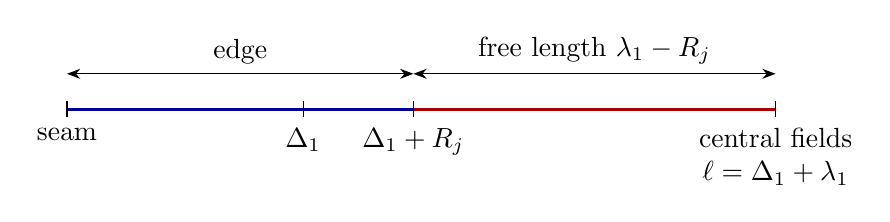
\begin{tikzpicture}[x=1cm,y=1cm,>=Stealth]
\draw[very thick,blue!60!black] (0,0)--(4.4,0);
\draw[very thick,red!65!black] (4.4,0)--(9,0);
\foreach \x in {0,3,4.4,9} \draw (\x,-.1)--(\x,.1);
\node[below] at (0,-.12) {seam};
\node[below] at (3,-.12) {$\Delta_1$};
\node[below] at (4.4,-.12) {$\Delta_1+R_j$};
\node[below,align=center] at (9,-.12) {central fields\\$\ell=\Delta_1+\lambda_1$};
\draw[<->] (0,.45)--node[above] {edge}(4.4,.45);
\draw[<->] (4.4,.45)--node[above] {free length $\lambda_1-R_j$}(9,.45);
\end{tikzpicture}

\caption{One real half-arc. The edge ends at $\Delta_1+R_j$;
its complement has length $\lambda_1-R_j$.}
\label{L:fig:two-scale}
\end{figure}

Sort the roots after the edge and denote the free gaps by $d_i'\ge0$.
On each arc their sum is $\lambda_1-R_j$. Their kinetic factors are
$e^{-E(y_i)d_i'}$, where $E(y)=y^2/(2H)$ and $H=9/4$. The momenta
change by positive integers in increasing real order; reversing the
parameterization on the other arc reverses all these changes. Thus,
for every fixed $B$, the number of gaps with $E(y_i)\le B$ is bounded
independently of $P$. Imaginary kinetic phases use only the fixed
angles and the edge data.

\paragraph{Exposing the long gaps.}
Fix a sufficiently large $s_0$, and let $B$ be an energy threshold to
be chosen below. A gap is active when
$E(y_i)\le B$ and $d_i'\ge s_0$. Expand every short interaction whose
directed path crosses an active gap, including image paths. First use
the frequency series for its logarithm and then exponentiate. Each
resulting path label contributes a nonnegative shift $\sigma_i$ to
 every crossed active rate and may contribute a polynomial in its
length from Jordan differentiation. All positive frequencies belong
to $\tfrac16\mathbb Z$, so every polynomial contribution is accompanied
by a positive shift. Interactions on paths crossing no active gap are
independent of active lengths and remain unexpanded.

The absolute sum of these expanded logarithms, even after reserving
half their frequency decay, is at most
\[
       \varepsilon\Bigl(1+\sum_I K_I^2\Bigr),
\]
where $\varepsilon$ is arbitrarily small for large $s_0$ and $K_I$
counts roots in unit bins. Indeed every such path has length at least
$s_0$; exponential frequency decay, including the polynomial Jordan
factors, is summable by bins. The same estimate bounds the cost of
deleting these paths from the intact product. The doubled stability
bound therefore still applies. It applies as well if active lengths
are varied independently above $s_0$: use the resulting circle, which
may have unequal half-arcs, with the same edge bend and angular
offsets. This is the estimate that allows some active lengths to be
set equal to $s_0$ below.

\paragraph{The bounds needed before extending coefficients.}
Fix the bend bound, distant-path margin, per-root exponential base and
retained kinetic fractions before choosing any accuracy threshold.
Then choose a clipping rate $b_1$ and much larger thresholds $A_2$ and
$B\ge A_2$. For each path label call an active gap cheap when
\[
                  e_i=E(y_i)+\sigma_i\le A_2.
\]
There are boundedly many cheap gaps, and their total polynomial degree
is bounded in terms of the thresholds: a polynomial power also costs
at least one positive frequency. Their rates range in a fixed finite
set, independent of $K_0$ and $P$.

We first collect the absolute estimates with the cheap lengths set
to $s_0$. In this substitution the absolute polynomial coefficients
are evaluated at $s_0$; the binomial expansion is bounded by the same
polynomial-in-path-distance majorant used above. Removing or restoring
the bounded cheap shifts and their kinetic factors at $s_0$ costs only
a threshold-dependent constant. The unused half of the path decay
controls high shifts. A further fraction of the kinetic energy
controls high original energies. To apply the root stability estimate
in the presence of probes, compare the actual kinetic momentum with
the root momentum; their difference is bounded. Borrowing a slightly
larger fraction of actual energy loses at most a fixed constant per
unit length. The distant-path and bend losses are absorbed by the
bin-square penalty. On the two edges the remaining loss is therefore
\[
              e^{C(2\Delta_1+R_L+R_R)},
\]
with $C$ fixed independently of the thresholds and Taylor accuracy.

By taking $A_2,B$ large enough, every noncheap gap that is long or
has high energy retains a penalty
\[
                   e^{-(b_1+\lambda_2)d_i'},
\]
where $\lambda_2$ can be any prescribed large fixed number. The only
other noncheap gaps have $E(y_i)\le B$ and $d_i'<s_0$; there are
boundedly many and their total length is bounded. Reserve a small
additional kinetic fraction for Gaussian tails in $f$ when there is
no cheap gap. If a cheap gap is present, its bounded momentum implies
$|f|\le C_B+CP$.

Here is the root-count summation with its constants made explicit.
Sorting cancels identical-root factorials. Species/order choices cost
$a_*^P$ for one fixed $a_*$, while marking the bounded number of low gaps
and summing allowed $f$ costs at most $(1+P)^{C_B}$. Use
\[
       (1+P)^{C_B}\le C'_B2^P;
\]
only the prefactor depends on $B$. If $l$ roots lie in one edge,
its ordered volume, in a unit bin of $R_j$, is bounded by
$(\Delta_1+\lceil R_j\rceil+1)^l/l!$. Consequently
\[
 \sum_{l\ge0}\frac{(2a_*)^l(\Delta_1+\lceil R_j\rceil+1)^l}{l!}
 =\exp\{2a_*(\Delta_1+\lceil R_j\rceil+1)\}.
\]
Arbitrary fixed exponential factors in $R_j$ are integrable by
localization. Each expensive integrated free gap contributes
$1/\lambda_2$ after the $b_1$ part of its penalty is reserved.
The number of free roots and free gaps differs by at most one on each
arc. Thus all but boundedly many free roots are paid for by these
integrated expensive gaps. Choose $\lambda_2$
to absorb the fixed exponential bases. These estimates give
$C_J e^{C\Delta_1}$ for the remaining data, with one exponent $C$
independent of $J$. No accuracy-dependent constant has been raised
to the unbounded number of edge roots.

\paragraph{Convolution, then extension.}
Suppose each arc has a cheap gap. For a fixed monomial in its cheap
lengths, convolve the factors $(d_i')^{k_i}e^{-e_i d_i'}$ exactly,
with $d_i'\ge s_0$ and sum
\[
            \lambda_1-R_j-\sum_{\rm other}d_i'.
\]
On its feasible interval the result is a finite exponential-polynomial
in this sum. This follows by translating the lower endpoints and
partial fractions of the Laplace transform. Its rates are among the
$e_i$, and the coefficient bounds depend only on the fixed finite rate
and degree set. Retain rates at most $b_1$.

The bounds just collected now justify extending their remaining
coefficient integrals to the product of their individual ranges: retain
$d_i'<s_0$ for inactive low-energy gaps and $d_i'\ge s_0$ for active
gaps, but remove their coupled sum constraint. A retained rate contributes
at most $e^{b_1R_j+b_1\sum_{\rm other}d_i'}$, times a bounded-degree
polynomial, to these coefficients. The reserved penalties on other
gaps and the arbitrary exponential moments of $R_j$ make this
integrable. Put $S_j=R_j+\sum_{\rm other}d_i'$. Beyond the old feasibility
boundary $S_j\ge\lambda_1-O_B(1)$. After paying $e^{b_1S_j}$,
reserve a further factor $e^{-tS_j}$, with $t$ as large as needed,
by the choice of $\lambda_2$ and the exponential moments of $R_j$.
The inactive low gaps have bounded total length. Hence the tail is
\[
 e^{-t(\lambda_1-O_B(1))}\,C_J e^{C\Delta_1},
\]
up to bounded-degree polynomial factors, and has any prescribed
exponential accuracy in $\lambda_1$. The discarded convolution rates
have the corresponding bound
\[
       e^{-b_1\lambda_1+b_1R_j+b_1\sum_{\rm other}d_i'}
\]
on the feasible interval, again with only bounded-degree polynomial
factors. If an arc has no cheap gap, its length constraint gives this
smallness directly; eliminate a last gap there rather than convolving.
The other arc costs at most the already bounded coefficient integrals
and polynomial factors. Extending the earlier restriction
$V_1\le\lambda_1/2$ is justified by its retained superexponential
penalty.

Thus the coefficient integrals are absolutely summable, and their
errors have arbitrarily high exponential accuracy in $\lambda_1$ at
cost $C_J e^{C\Delta_1}$. Since
$\lambda_1=6\log s_1$ and $\Delta_1=6\log K_0$, this is the claimed
$C_JK_0^{C_2}s_1^{-J}$ form, with fixed $C_2$. The large clipping rate
has multiplied $R_j$, whose exponential moments change only $C_J$;
it has not multiplied $\Delta_1$.

\par\medskip\noindent\textbf{Minimal rates.}
What remains is polynomial powers in \(\lambda_1\) times rates \(e_L+e_R\) chosen among the cheap rates on the respective arcs (and the earlier nonnegative Taylor orders). Coefficients retain the stated bounds and holomorphy, since other positions, signs of real orders, angular parameters and phase classes in these prescriptions are fixed independent of \(\lambda_1\) and the composition in its neighborhood. Uniformity along the bounded imaginary shifts allows Cauchy averaging. For \(p_*=2\), between selected gaps in increasing real order across the center one gains \(3/2\) from the marks and only nonnegative other changes. Hence \(E(y_L)+E(y_R)\ge1/4\), giving \(\gamma\ge6/4\). At equality there is no Taylor correction and the two shifts vanish; the chosen momenta are \(-3/4,3/4\). No changing roots are between these gaps and the marks (uncoupled roots in the free region all change the momentum positively in increasing real order), so all other free gaps have strictly larger kinetic energy on their respective arcs. Thus both convolution poles are simple, with no contributing polynomial powers there since a path crossing either would shift its rate. For \(p_*=0\), momenta are in \(f_0+\mathbb Z\), giving \(6(E(y_L)+E(y_R))\ge1/6\), equality only for \(y_L=y_R=f_0\). For that order there can be no shifts or Taylor corrections and each convolution pole is simple without path powers by strict unit-or-larger changes along the relevant free gaps. Changing a momentum costs at least \(6/9\) in exponent, and positive shifts or Taylor powers at least \(1/2\). This proves \eqref{L:eq9}.


\end{proof}

\subsection{Physical interpolation}\label{L:step16}

First in the unmarked case the comparison \(|Q|\ge c_1{\cal D}\) forces nonvanishing of the leading coefficient, locally even at nonrational limiting compositions. Indeed fix any possible residue class of the family/angle counts occurring along an infinite sequence. To approach an admissible limit on it one can take the counts within bounded error of the exact scaled composition, preserving residues (and orientation at a tie if needed). One can use either nearly equal splitting since the identity computes the symmetric \(Q^2\) regardless of the chosen split. If the coefficient there vanished, holomorphy gives error \(O(1/|Z|)\) in evaluating it along this approximation, contradicting the comparison since \(5/24=3/8-1/6<1/2\). Compactness thus gives
\[
 |Q(Z)|^2\asymp {\cal D}(Z)^2 |Z|^{5/24}.
\]
Also the mass \(C_a\) of loops visiting just a prescribed mark (no constraint at other sites) is bounded above by a constant at any such physical list. Use the one-port mark reduction to \(E_+(Z;t)\) at \(t=a\) (take the seam there). By its formula and the cap reduction for \(Q(Z,q^3a)\) the nonconstant term is a bounded prefactor times \(Q(Z,a)Q(Z\setminus a)/Q(Z)^2\). The just-proved estimate gives the bound since the products in \({\cal D}\) cancel up to fixed factors. In particular \(0\le C_{ab}\le C_a\le C\).

For bounded $K_0$, equation~\eqref{L:eq9} now gives~\eqref{L:eq8}
directly. For large integral $K_0$, put $m_0=K_0^{1/4}$. We calibrate
the marked expansion using physical values near this smaller scale.
Choose one sufficiently large accuracy $J>4C_2+1$ and keep its finite
rate and degree list fixed. At $m_0$ the remainder satisfies
\[
 K_0^{C_2}m_0^{-J}=o(K_0^{-5/24})
                   =o((K_0m_0)^{-1/6}).
\]
The strict power margin also absorbs any fixed logarithmic factor.

\paragraph{Interpolating the angle fraction.}
Fix a target phase class and common physical fraction $\theta$.
At each of finitely many sizes $m'$ near fixed multiples of $m_0$,
choose an integer $m'$ within bounded error preserving the size class.
Use equally spaced neighboring admissible later counts $j'$ of the
prescribed class in the first family, and exactly $K_0j'$ in the second.
Choose them within bounded distance of $m'\theta$ and within the physical
range; one-sided choices suffice at an endpoint. The bound $C_{ab}\le C$
and the unmarked $Q$ estimate imply
\[
 |G_Z^{(2)}|\le C(K_0m_0)^{-1/6}
\]
at these physical points. Formula~\eqref{L:eq9} gives the same bound for
its truncated expression there.

Interpolate that expression in the common angle parameter. A fixed
sufficiently large number of the neighboring grid points has bounded
interpolation weights. Holomorphy and the coefficient bound give a
derivative remainder at most
\[
 C_JK_0^{C_2}(1+\log m_0)^{C_J}m_0^{-A}
\]
for any prescribed fixed interpolation order $A$. Choose $A$ large
enough that this and the formula errors are negligible. We have therefore
bounded the truncated expression at the exact target fraction $\theta$,
without a divisibility requirement on $m'\theta$.

\paragraph{Interpolating the size.}
Write $m=m_0e^u$. The truncated expression is a linear combination of
the finitely many functions $e^{-\gamma u}u^i$ in its fixed rate and
degree list. Choose fixed evaluation values of $u$ for which their
matrix is invertible; linear independence guarantees such a choice.
The bounded rounding of each $m'$ perturbs these values by $O(m_0^{-1})$,
so the inverses stay bounded. Thus every coefficient in this shifted
basis, including its factor $m_0^{-\gamma}$, is
$O((K_0m_0)^{-1/6})$ at the exact target composition.

For $u\ge0$, the higher-rate polynomial terms are bounded by a constant
times $e^{-3u/2}$. At the rate $3/2$ there is no polynomial factor.
Consequently
\[
 |G_Z^{(2)}|\le C(K_0m_0)^{-1/6}(m/m_0)^{-3/2}
                       +O_J(K_0^{C_2}m^{-J}),\qquad m\ge m_0.
\]
Undo the normalization, using $|Z|\asymp K_0m$ and the unmarked
$Q$ estimate. The principal term gives
\[
 C_{ab}\le C(K_0m)^{1/6}(K_0m_0)^{-1/6}(m/m_0)^{-3/2}
       =C m^{-4/3}K_0^{1/3}.
\]
The remainder relative to this target is at most
$C_JK_0^{C_2+5/24-J/4}$ for $J\ge3/2$, so the same choice of $J$
absorbs it. All choices can be made on fixed local neighborhoods;
a finite cover of the composition interval makes the constant uniform.
This proves~\eqref{L:eq8}.

\subsection{The polygon second moment}

We now convert the two-port estimate into a bound on all ordered vertex
pairs of a polygon. Good displacements are counted directly; polygons
concentrated near a lattice side line require a separate width argument.
For plane honeycomb polygons \(P\), modulo primitive lattice translations,
the resulting estimate is
\begin{equation}
 \sum_{R\le{\rm diam}\,P<2R} X^{|P|}|P|^2\le C R^{2/3}(1+\log\log R).\label{L:eq10}
\end{equation}
\paragraph{Pairs away from lattice side lines.}
Call ordered vertex pairs good for displacements of length at least \(R^{1/3}\) and at Euclidean distance greater than a sufficiently large fixed constant from all lattice side lines through zero. To count their weighted mass fix the first polygon vertex (either type) and sum over displacements to the other. A good displacement is well inside some rotated \(e_0,e_1\) cone. At each visited vertex the polygon uses two of three midports and therefore at least one oriented-side choice in these two directions. Sum over both choices there. For any prescribed such pair, one forward zigzag can include those two sides: between the end of the first and start of the second is a nonnegative integral combination of \(e_0,e_1\). If it takes \(m\) steps, \(m\) is comparable to the distance. On the rest of the zigzag period after the second mark take \(K_0\) copies of the intermediate step counts, \(K_0\asymp R/m\) integral and large enough that the period vector has length \(>4R\). Reflection exchanging the side directions allows the later proportion \(\le1/2\). Projection now embeds all the required polygons injectively at the marks (lift at the first mark), preserving physical weights. Thus \eqref{L:eq8} applies since \(m\gtrsim R^{1/3}\). At dyadic displacement scale \(r\) this costs \(R^{1/3} r^{1/3}\) up to constants. Hence \eqref{L:eq10} holds with the good-pair count in place of the squared length.

\paragraph{Polygons concentrated near a side line.}
We can discard with superpolynomial length-weighted accuracy polygons of transverse width below \(R/\log^2 R\) relative to any lattice side direction. Project these contractibly to a cylinder along a different (nonparallel) lattice side with period \(\lceil C R/\log^2 R\rceil\), \(C\) large fixed; translates do not meet by the width bound, whereas the height there is of order at least \(R\). The exponential pressure height estimate applies, also with length powers, and a plane polygon modulo translations is recovered by lifting.

For length \(l\gtrsim R\), short displacements account for \(O(lR^{2/3})\) pairs. If there is not already a fixed positive fraction good, some constant-width band through one vertex parallel to a lattice side then contains a positive fraction of all vertices by pigeonhole, implying \(l=O(R)\). Group these exceptional polygons by that side direction and dyadic transverse width \(w\gtrsim R/\log^2R\) relative to it. At least \(c w\) vertices lie at distance \(\gtrsim w\) from the band, by the width and bounded step size. For each, the other-direction side-line tubes through it meet the band in bounded regions, and a sufficiently small constant times \(R\) as minimum displacement length still leaves a positive fraction of the band vertices giving good partners (the band has constant width). Thus at least a fraction \(c' w/R\) of all ordered pairs are good with displacement of order \(R\), transverse component at most \(Cw\). There are only \(O(wR)\) such displacement vectors and each costs \(O(R^{-4/3})\) by the argument above. The good-pair mass in this bin is therefore at most
\[
 C(wR)R^{-4/3}=CwR^{-1/3}.
\]
Each such polygon has at least $c(w/R)|P|^2$ good pairs, so its
squared-length mass, summed over the bin, is at most
\[
 C\frac{R}{w}\,wR^{-1/3}=CR^{2/3}.
\]
Only $O(1+\log\log R)$ width bins lie between $R/\log^2R$ and $O(R)$.
Together with the ordinary good-pair estimate and the negligible thin
polygons, this proves~\eqref{L:eq10}.


\section{Positive bridges, caps, and growth}\label{L:part10}

We now turn the partition estimates into positive families of open paths. The immediate goals are transverse tightness, length-controlled half-plane growth with recoverable cuts, and caps at prescribed boundary gaps. These are the geometric inputs needed to convert a long arch into a bridge without losing more than logarithmic factors. Use triangle-center walks with boundary endpoints at midports, weight \(X^{|\omega|}\) per walk (\(|\omega|\) counts centers), so gluing at a midport multiplies weights. Triangle-side levels in any fixed lattice direction are numbered at unit spacing (one interline distance as unit). A strict bridge of height \(h\ge1\) goes from a fixed port on level 0 to level \(h\), with all its centers strictly between. By Proposition~\ref{L:prop:strip-mass} its total mass is \(B_h\asymp h^{-1/4}\); include \(B_0=1\). Reflection/translation give the same conventions in any of the side directions. The arch on a half plane is a nonempty return to the source side before any other contact, and \(A_g\) denotes its mass to a port at positive horizontal gap \(g\) (one of the two displacements), integer in lattice side lengths.

We recall the useful clipping rule: for a boundary port of a finite convex domain of triangles with straight sides, exit flux with coefficient \(\cos((3/8)\,{\rm turn})\) is 1 by the extension identity. Coefficients are fixed by boundary tangents and uniformly positive. Cutting such a domain by a lattice side line (keeping the source) thus bounds the mass of all lost exits, including excursions of arcs to retained endpoints past the cut, by a constant times new exits at the cut; conversely positive lost terms give lower bounds on these new exits. Indeed coefficients to shared endpoints agree. More generally on a simple polygonal domain made of triangles with the source on its outer (counterclockwise) boundary, the same complex identity from the finite proof holds: collision detours are approached from outside so still cancel. If \(\alpha\) is the tangent angle at an exit port lifted by following this boundary from the source (angle measured from the starting boundary tangent), the path turn to that port is \(\alpha-\pi\), by closing counterclockwise from there to the source (the two extra corners are \(+\pi/2\) each). In the straight strip the identity \(1=\cos(3\pi/8) A^{[h]}+B_h\) holds as in the strip calculation, \(A^{[h]}\) summing both directions of return. Thus total half-plane arch mass is \(1/\cos(3\pi/8)\), and the arch height tail has order \(B_h\).

Here are two tightness consequences with fixed constants.
\begin{enumerate}
\item Arch mass of diameter \(>r\) is \(\le C r^{-1/4}\). Take an equilateral triangle of side order \(r\), slightly smaller than \(r\), with horizontal base. For a source in the central third of the base compare to the half-plane identity. All arches of diameter \(>r\) are lost, hence bounded by exits on the other sides. Average over base sources there and reverse from those sides: for each other-side port, arcs ending on the central base must penetrate to normal distance \(c r\) or larger from that port's side. Clipping by a parallel line at such distance thus bounds their sum by \(C B_{\lfloor c'r\rfloor}\). There are \(O(r)\) ports on the other sides, proving the bound.
\item Bridges of height \(d\) remaining at transverse displacements at most \(Td\) from the source's normal have mass \(\ge c d^{-1/4}\) uniformly for sufficiently large fixed \(T\), even specifying either weak sign for the endpoint displacement from that normal. Indeed clip the strip at lateral distance of order \(S\gg d\) by two slant lattice side lines. Mass lost is bounded by lateral exits by the strip identity. Those exits are included in the analogous half-plane clip with same lateral lines and a distant parallel top at height \(\asymp S\). There the half-plane identity bounds their sum by lost arches, all of diameter \(\gtrsim S\). This proves tightness by the preceding estimate; for a sign use reflection symmetry in the source's normal.
\end{enumerate}

The enclosing-loop estimate supplies length control for the growth
construction below. We record its finite-domain consequence before choosing
the growth prefixes, so that length can be included in their cut tests.

\begin{proposition}[Finite chord length mass]\label{L:prop:box-moment}
For every finite convex domain of triangles with a bounded number of
lattice sides and diameter at most $C_0r$, the critical length-weighted
mass of all boundary-to-boundary chords, with both endpoints summed, is
at most $C r^{25/12}$. In particular, for a fixed $T$, the length-weighted
mass of strict bridges of height $d$ from one fixed source and transverse
displacement bounded by $Td$ is at most $C_Td^{13/12}$.
\end{proposition}
\begin{proof}
By the plane ball upper bound following \eqref{L:eq1} and the visit comparison \eqref{L:eq6}, for a finite convex polygonal domain as there of diameter \(O(r)\) with boundedly many lattice sides, the sum of chordal masses times length, over all sources and exits, is \(O(r^{2+1/12})\) by the ball upper bound. Centers right at the boundary where \eqref{L:eq6} may not apply number \(O(r)\), costing only \(O(r^2)\) since total exit mass per source is bounded. In particular bridges of height \(d\) from a fixed source staying within transverse displacement \(Td\) as in tightness have length-weighted mass at most \(C_T d^{13/12}\). Indeed shift them to order \(d\) distinct sources in a common larger such box with the same two strip walls.
\end{proof}

A cut is read at a port on a lattice-side grid line. In the forward
paths considered below, each candidate \(u\)-level lies between the
starting and terminal levels. An interior candidate is a
\emph{single-crossing cut} if the path crosses it at exactly one port.
A terminal candidate is treated as a cut when all centers lie on its
starting side; it becomes single crossing after an extension strictly
beyond that wall. The \emph{first qualifying cut} is the lowest candidate
with this cut property whose prefix satisfies the specified diameter,
confinement, terminal-position, and, when present, length conditions.
These auxiliary conditions concern the prefix alone. If \(u=t\) is
selected, every center of the suffix lies in \(u>t\), or the suffix is
empty at a terminal cut. Removing that suffix or replacing it by another
extension in \(u>t\) changes neither the crossing counts at earlier
candidates nor their prefix conditions, and the selected level remains
eligible as a terminal or single-crossing cut. Thus the first-cut rule
recovers the same cut.

\begin{unnumberedproposition}[Recoverable half-plane growth]
\phantomsection\label{L:prop:recoverable-growth}
\label{L:prop:length-controlled-growth}
Let \(n,u\) be signed normal level coordinates in two lattice directions
whose unit inward vectors have dot product \(1/2\). Let \(A\) be a port
on the \(n=0\) wall, and measure both coordinates relative to \(A\).
There are constants \(r_0,c,C,c'>0\), independent of \(r\), such that
for every \(r\ge r_0\) there is a family of distinct prefixes from \(A\)
with total critical mass at least \(c\), whose terminal \(u\)-levels
\(s\) lie in the grid bin \([r,2r]\). Every prefix has all centers in
\(n>0\) and \(u<s\), diameter at most \(Cr\), center length at most
\(Cr^{4/3}\), and terminal \(n\)-coordinate at least \(c'r\).
Its terminal cut is selected by the first-cut rule and is recoverable
after any extension strictly beyond it in \(u\).

For each fixed sufficiently small \(\gamma>0\), there are a threshold
\(r_\gamma\ge r_0\) and positive constants \(K_\gamma,c_\gamma,C_\gamma\),
and \(C_{1,\gamma}\) such that, for every \(r\ge r_\gamma\) and every
admissible grid target \(S\ge K_\gamma r\), these prefixes can be
continued to the exact wall \(u=S\), with terminal port free, so that
all centers remain in \(n>0\) and \(u<S\), the diameter is at most
\(C_\gamma S\), the center length is at most \(C_\gamma S^{4/3}\),
and the resulting family has total mass at least
\[
 c_\gamma S^{-1/4}(S/r)^{-C_{1,\gamma}}.
\]
During the continuation, the transverse distance from the positive
\(u\)-normal ray through the selected prefix endpoint is at most
\(\gamma u\). The cuts separating all stages are recovered by the same
first-cut rule.
\end{unnumberedproposition}

The length restrictions will be needed for the final exterior connectors.
The cap construction below uses only the mass, geometry, and recovery
conclusions; retaining the length restrictions costs only fixed constants.

\begin{proof}
\textbf{Initial exits and the first cut.}
Fix a target grid level \(s\in[r,2r]\). Truncate the half-plane \(n>0\)
to a finite convex domain of diameter \(O(r)\) that contains the arches
of diameter at most \(C''r\) used below, and clip it at \(u=s\).
The half-plane height tail supplies arch mass at least \(cr^{-1/4}\)
reaching \(n>8r\). Choosing \(C''\) large retains a fixed fraction by
the arch diameter tightness. Reflection in the starting \(n\)-normal
ray shows that at least half of this retained mass crosses the clipping
line. The positive clipping identity therefore supplies exits at \(u=s\)
of mass at least \(cr^{-1/4}\).

We need the endpoint to be a positive distance inside \(n>0\).
Translate the domains along the \(n\)-wall so that all target \(u\)-walls
in the bin coincide. The starting ports then become distinct. On that
common wall there are \(O(1+c'r)\) ports with \(n<c'r\). Reverse paths
from each such port. They are included in a common finite convex
truncation between the two walls, and reaching the translated starting
ports costs at most \(Cr^{-1/4}\) per reversed source: clip at a line
parallel to the aligned \(u\)-wall at distance of order \(r\), then use
the bridge upper bound. Thus the total shallow-endpoint mass in the bin
is at most \(C(1+c'r)r^{-1/4}\). The exits over all levels in the bin
have mass at least \(cr^{3/4}\); choose \(c'\) small and then \(r\)
large to retain that order of good exits.

These translated exits are boundary chords in one finite convex domain
of diameter \(O(r)\), after enlarging its other sides by a fixed factor.
Proposition~\ref{L:prop:box-moment} bounds their total length-weighted
mass by \(Cr^{25/12}\). Exits of length greater than \(Mr^{4/3}\)
therefore have mass at most
\[
 (Mr^{4/3})^{-1}Cr^{25/12}=(C/M)r^{3/4}.
\]
Choose the fixed \(M\) large enough to retain a positive fraction of
the good exits. Undo the translations, so that they again start at \(A\).

For each retained exit, keep the prefix to its first qualifying
\(u\)-cut in the bin. The tests are the diameter bound, \(n>0\)
confinement, terminal-depth bound, and length at most \(Mr^{4/3}\).
All concern the prefix alone, and the final wall qualifies. After a
candidate single crossing, the discarded suffix is a strict
\(u\)-bridge, and its total possible mass over the target levels is
at most
\[
 \sum_{0\le d\le2r}B_d=O(r^{3/4}).
\]
Consequently the distinct selected prefixes have total mass at least
a positive constant. Their lengths are at most \(Mr^{4/3}\).
The selected prefix and every earlier test are unchanged on extension
strictly beyond its cut, so that cut remains recoverable.

\smallskip\noindent\textbf{Length-controlled increments.}
Fix the transverse confinement constant \(T\) from the tightness
estimate. A strict bridge of increment \(d\) within that confinement
has mass at least \(cd^{-1/4}\), even with either specified weak
terminal sign. The whole confined family has length-weighted mass
at most \(C_Td^{13/12}\), by Proposition~\ref{L:prop:box-moment}.
Thus imposing length at most \(M_1d^{4/3}\) loses at most
\((C_T/M_1)d^{-1/4}\) from either sign-restricted family. Choose
\(M_1\) once, large enough for the confinement and sign constants.
Every increment family below then retains its original mass order.

Now start from a selected cut at \(u=t\). Choose a small fixed
\(\zeta>0\), with its value in terms of \(\gamma\) fixed below.
After fixing \(\zeta\), take \(r_\gamma\) large enough that the integral
increment bins below have their asserted order of cardinality and any
fixed lattice-scale rounding errors are absorbed by the transverse bound.
While \(t\le S/(1+3\zeta)\), use strict \(u\)-bridges
of integral increment \(d\in[\zeta t,2\zeta t]\). Require transverse
displacement at most \(Td\) from the increment's starting normal and,
if the current endpoint is off the initial \(u\)-normal ray, require
the weak sign pointing toward that ray. With the length restriction
just imposed, their mass over the bin is at least
\(c_\zeta t^{3/4}\).

Extract first qualifying cuts in this increment bin, allowing the
terminal wall and testing
transverse displacement at most \(2T\zeta t\), the selected terminal
sign, and prefix length at most \(M_1(2\zeta t)^{4/3}\).
These tests depend on the current starting cut and its prefix, not on
the discarded terminal target \(d\). Every retained increment has
its terminal wall eligible. The suffix sum is again
\(O_\zeta(t^{3/4})\), so the distinct increment prefixes have mass
at least \(c'_\zeta>0\), and their cuts are recoverable.

Each such stage increases \(t\) by at least \(\zeta t\), so there are
\(O_\zeta(1+\log(S/r))\) stages. At the first larger \(t\), the
remaining increment \(S-t\) is comparable to \(\zeta S\); finish
with a strict bridge at that exact height, with the same confinement,
weak terminal sign, and length restriction. It has mass at least
\(c_\zeta S^{-1/4}\). The weak signs keep endpoint errors bounded
by the largest increment-width bound used so far; within a stage the
additional error has the same order. Thus the continuation stays
within \(O(T\zeta u)\) of the initial ray. That ray begins at
\(n\ge c'r\) and gains \(n\)-clearance at slope \(1/2\).
Choose \(\zeta\) small enough in terms of \(\gamma,c',T\).
All stages then remain in \(n>0\), the diameter is \(O(S)\),
and strict slabs keep new centers beyond the preceding cuts and
before the target wall.

The starting levels of successive stages grow geometrically.
Their prefix-length bounds therefore sum to \(O_\gamma(S^{4/3})\).
The final increment is comparable to \(\zeta S\), so its length and
the initial \(O(r^{4/3})\) contribution obey the same bound.
Critical weights multiply at the joining ports. The first-cut rule
recovers the stages from the output, so multiplying their lower bounds
does not create an unaccounted multiplicity. A fixed positive factor
for each of \(O_\zeta(1+\log(S/r))\) stages, followed by the exact
final bridge, is at least
\(c_\gamma S^{-1/4}(S/r)^{-C_{1,\gamma}}\).
This proves every asserted conclusion.
\end{proof}

We next construct caps at prescribed gaps.  The first step gives a
lower bound at some gap on each scale.  A one-cell-thick boundary
deformation then compares any smaller prescribed gap to that one.

\begin{unnumberedproposition}[Caps at prescribed gaps]
\phantomsection\label{L:prop:caps}
There are constants $c,C>0$ such that, for every integer $g\ge1$,
\[
 \sum_{\substack{\omega\text{ an arch at gap }g\\
                  \operatorname{diam}\omega\le Cg}}
       \mu(\omega)\ge c g^{-5/4}.
\]
Moreover, the unrestricted arch masses satisfy
$A_g\ge c A_q$ whenever $1\le g<q$.
\end{unnumberedproposition}
\begin{proof}
\medskip\noindent\textbf{A gap with substantial mass on each scale.}
We first show that, for every sufficiently large $r$, some integer
$q'\in[\lfloor r\rfloor,Cr]$ has arch mass at least $cr^{-5/4}$
with diameter at most $Cr$.
Use level coordinates $Y,U_+,U_-$ whose normals have angles
$\pi/2,\pi/6,-\pi/6$, respectively.  With a lattice vertex as origin
and one interline distance as unit, $U_-=U_+-Y$, and the integer levels
are lattice-side grid lines.  Put the source at the midpoint of
$[0,1]$ on $Y=0$, using horizontal lattice-side length one.  Set
$p=\lfloor r\rfloor$.  Choose integers $S,M$ that are successively
large fixed multiples of $r$, up to rounding, and let $D_r$ be the
finite triangle domain
\[
 Y\le M,\qquad -M\le U_-\le S,\qquad
 (Y\ge0\ \text{or}\ U_+\ge p).
\]
Its lower boundary travels east to position $p$, then down-right
along $U_+=p$ to the wall $U_-=S$.  That wall rises up-right to the
top.  Clipping by $Y\ge0$ replaces this lower excursion by the
horizontal segment from $p$ to $S$.

Let $\alpha$ be the tangent angle lifted along the counterclockwise
outer boundary from the source, as in the boundary-flux identity.
In $D_r$ its values lie in $[-\pi/3,2\pi]$; the clipped domain has
the same lifts at shared boundary ports.  Rotate the complex identity
by $\exp(i(3/8)\pi/6)$ and take real parts.  The exit coefficient is
\[
 \cos\!\left(\frac38\left(\alpha-\frac{5\pi}{6}\right)\right)
 \ge\cos(7\pi/16)>0
\]
throughout both domains.  Consequently the mass of exits removed by
the clipping gives a lower bound, up to a fixed factor, for the mass
of exits on its new horizontal segment.  Indeed shared coefficients
agree, and enlarging the domain only increases the path mass at a
shared exit.

We produce removed exits of mass at least $cr^{-1/4}$.  Apply the
initial-prefix part of recoverable half-plane growth with normals
$(Y,U_+)$ and scale $2r$.  The resulting prefixes have constant total
mass, diameter $O(r)$, and terminal absolute $U_+$-level greater
than $p$.  From each terminal port apply the full growth construction
with normals $(U_+,U_-)$, initial scale $r$, and exact absolute target
$U_-=S$.  All new centers lie strictly beyond the first cut in $U_+$.
They are therefore disjoint from the first prefix and remain in the
additional part of $D_r$ even when $Y<0$.  The ratio $S/r$ is fixed,
so the second construction has mass at least $cr^{-1/4}$.

Along a positive $U_-$-normal ray, $Y$ decreases at rate $1/2$.
The initial stages contribute an $O(r)$ displacement and the
continuation contributes transverse error $O(\gamma S)$.
Choose $\gamma$ small, then $S/r$ large enough that the terminal
port lies below $Y=0$.  Finally choose $M/r$ still larger so that
all paths fit below the top and to the right of the other wall.
The exact-target property keeps all centers before $U_-=S$.
The first $U_+$-cut is recovered from the output because the second
part lies strictly beyond it.  Hence multiplying the two family
weights introduces no additional multiplicity.  We have obtained
the claimed mass of exits on the removed part of $U_-=S$.

Subtracting the two rotated flux identities now gives at least
$cr^{-1/4}$ mass on the new horizontal segment of the clipped domain.
These paths are arches, have diameter $O(r)$, and end at only $O(r)$
possible gaps in $[p,S]$.  One gap $q'$ therefore has the asserted
mass $cr^{-5/4}$.

\medskip\noindent\textbf{Gap comparison.}
\phantomsection\label{L:cap-gap-comparison}
Fix integers $1\le g<q$, put $p=g+1$, and let $D$ be a large finite
convex triangle domain above the horizontal base.  Its base contains
the source $1/2$ and the target $q+1/2$.  Write $A_q(D)$ for the
mass of arches between these ports contained in $D$.  In complex
coordinates put $w=e^{-i\pi/3}$ and add the one-cell-thick bump
\[
 [p,q+1]+[0,w]
\]
below the base.  Equivalently, add the rhombi
$j+[0,1]+[0,w]$, $j=p,\ldots,q$.  Call the enlarged domain $D'$.

Figure~\ref{L:fig:cap-comparison} shows the added cells and the fixed
extensions used below.
\begin{figure}[htbp]
\centering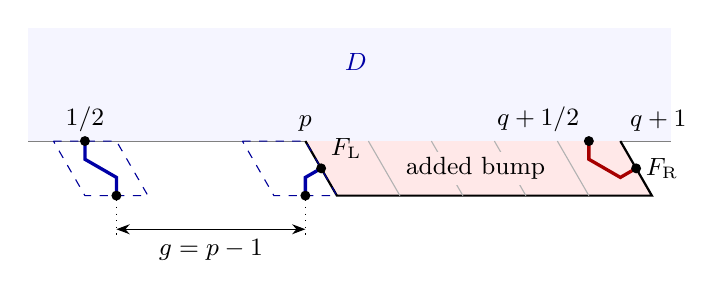
\begin{tikzpicture}[x=.8cm,y=.8cm,>=Stealth,font=\small]
 \fill[blue!4] (-.4,0)--(9.8,0)--(9.8,1.8)--(-.4,1.8)--cycle;
 \node[blue!65!black] at (4.8,1.25) {$D$};
 \draw[gray] (-.4,0)--(9.8,0);
 \fill[red!9] (4,0)--(9,0)--(9.5,-.866)--(4.5,-.866)--cycle;
 \draw[thick] (4,0)--(4.5,-.866)--(9.5,-.866)--(9,0);
 \foreach \j in {5,6,7,8} {
   \draw[gray!60] (\j,0)--({\j+.5},-.866);
 }
 \foreach \j in {0,3} {
   \draw[dashed,blue!60!black] (\j,0)--({\j+1},0)--({\j+1.5},-.866)--({\j+.5},-.866)--cycle;
 }
 \draw[very thick,blue!65!black] (.5,0)--(.5,-.289)--(1,-.577)--(1,-.866);
 \draw[very thick,blue!65!black] (4.25,-.433)--(4,-.577)--(4,-.866);
 \draw[very thick,red!65!black] (8.5,0)--(8.5,-.289)--(9,-.577)--(9.25,-.433);
 \fill (.5,0) circle(1.8pt) node[above] {$1/2$};
 \fill (8.5,0) circle(1.8pt) node[above left] {$q+1/2$};
 \fill (4.25,-.433) circle(1.8pt) node[above right] {$F_{\rm L}$};
 \fill (9.25,-.433) circle(1.8pt) node[right] {$F_{\rm R}$};
 \fill (1,-.866) circle(1.8pt);
 \fill (4,-.866) circle(1.8pt);
 \draw[dotted] (1,-.94)--(1,-1.55);
 \draw[dotted] (4,-.94)--(4,-1.55);
 \draw[<->] (1,-1.4)--node[below] {$g=p-1$}(4,-1.4);
 \node[fill=red!9,inner sep=2pt] at (6.7,-.43) {added bump};
 \node[above] at (4,0) {$p$};
 \node[above right] at (9,0) {$q+1$};
\end{tikzpicture}

\caption{Local geometry of the gap comparison, shown for $p=4$ and $q=8$.
The shaded bump enlarges $D$ to $D'$. The red extension sends a path
ending at $q+1/2$ to the right slant port. The two blue extensions use
the dashed cells outside $D'$ to turn a path to the left slant port
into an arch of gap $g=p-1$. The labels $F_{\rm L},F_{\rm R}$ denote
exit masses at the slant ports.}\label{L:fig:cap-comparison}
\end{figure}

Use the complex flux identity at the same source in $D$ and $D'$,
multiply it by $e^{i(3/8)\pi}$, and take imaginary parts.  An exit
with lifted tangent angle $\alpha$ now has coefficient
$\sin(3\alpha/8)$.  On the left slant of the bump,
$\alpha=-\pi/3$, giving $-\sin(\pi/8)$; on its right slant,
$\alpha=2\pi/3$, giving $\sin(\pi/4)$.  The bottom horizontal
ports and the remaining horizontal ports to the right of the source
have coefficient zero.  At every other shared boundary port the
coefficient is unchanged and nonnegative, since the convex boundary
lifts lie in $[0,2\pi]$.

Let $F_{\rm L}$ and $F_{\rm R}$ be the masses of paths from the
source to the left and right slant ports of the bump in $D'$.
Subtract the identity in $D$ from the one in $D'$.  The right-hand
sides agree, and the mass at a shared port can only increase.  Thus
\[
 \sin(\pi/8)F_{\rm L}\ge\sin(\pi/4)F_{\rm R}.
\]
Every arch counted by $A_q(D)$ can be extended through the last bump
cell, cell $q$, to the right slant port.  This adds a bounded number
of centers in a previously unused region and is recoverable by
deleting that fixed extension.  Hence $F_{\rm R}\ge cA_q(D)$.

Conversely, extend a path counted by $F_{\rm L}$ through cell $p-1$
to that cell's bottom port, and extend its source backwards through
cell $0$ to the bottom port there.  Both cells lie outside $D'$ and
are distinct because $p\ge2$, so these extensions avoid the path
and each other.  The new endpoints are
\[
 \frac12+w\qquad\text{and}\qquad p-\frac12+w.
\]
Their gap is $p-1=g$.  All centers are strictly above the common
bottom line; translating by $-w$ gives an arch at gap $g$ in the
original half-plane.  The fixed extensions have bounded weight cost
and bounded inverse multiplicity.  Therefore
\[
 A_g\ge cF_{\rm L}\ge cA_q(D).
\]
The constants are independent of $D,g,q$.  Exhausting the half-plane
by such domains proves the unrestricted comparison $A_g\ge cA_q$.
This comparison applies to all paths at the farther gap, without a
diameter restriction.  If $q=O(r)$ and the input arches are contained
in a domain of diameter $O(r)$, the bump and both extensions also
have diameter $O(r)$, so the comparison preserves such a cutoff up
to a fixed factor.

For large $g$, apply the first part with $r=g+1$.  It gives
$q'\ge g+1$ with mass at least $cg^{-5/4}$ and diameter $O(g)$.
Use the finite-domain version of the gap comparison to obtain the
same lower bound at $g$, still with diameter $O(g)$.  The finitely
many smaller gaps follow by choosing one sufficiently large fixed
$r$ and adjusting $c,C$.  This proves the proposition.
\end{proof}

The same comparison gives the pointwise upper bound. For large $g$,
each of order $g$ integer gaps $j\in[g/2,g)$ satisfies $A_j\ge cA_g$.
Every arch at such a gap has diameter at least $g/2$, so the diameter
tail proved above gives
\[
 gA_g\le C\sum_{g/2\le j<g}A_j\le Cg^{-1/4}.
\]
Thus $A_g\le C(1+g)^{-5/4}$, with bounded gaps absorbed by changing $C$.

\subsection{Critical irreducible bridges}\label{L:step17}

As a separate consequence of the finite bridge bounds, we obtain the
classical irreducible-bridge law. The following result is not needed for
the logarithmic window proved in the next section. We use the classical
construction \cite{Kesten1963,MadrasSlade1993}. Its critical normalization
and independent concatenation in the honeycomb mid-edge convention are
also given in \cite[Appendix]{BeatonEtAl2014}; the finite bridge bounds
here yield the additional quantitative tails below.
Cutting a strict bridge at all its intermediate single-crossing levels
decomposes it uniquely into strict bridges with no intermediate
single-crossing level; these are the \emph{irreducible bridges}. The cuts are ordered by height.
Each portion lies strictly between its two cut lines: a return past a
line would cross it again. Conversely, irreducible pieces concatenate
freely, translating the next starting port to the previous terminal
port. Their center sets lie in disjoint open slabs, so the concatenation
is self-avoiding and its critical weight is the product of the weights.

\begin{proposition}[Critical irreducible law]\label{L:prop:irreducible}
The sum of $X^{|\gamma|}$ over irreducible strict bridges $\gamma$ from a
fixed port is one. Under this probability law, if $Y$ and $D$ are the
height and diameter of the sampled bridge, then
\[
 1-\mathbb E e^{-tY}\asymp t^{3/4}\quad(0<t\le1),\qquad
 \Pr(D>r)\le C r^{-3/4}\quad(r\ge1).
\]
Independent samples may be concatenated to form an infinite
self-avoiding port path.
\end{proposition}
\begin{proof}
Let $i_j$ be the total irreducible mass at height $j\ge1$. Unique
factorization gives the identity of nonnegative power series
\[
 \sum_{h\ge0}B_hz^h=\sum_{k\ge0}\left(\sum_{j\ge1}i_jz^j\right)^k.
\]
For $z=e^{-t}<1$ the left side is finite, since $B_h\asymp h^{-1/4}$.
Consequently $I(t)=\sum i_j e^{-tj}<1$ and
\[
 1-I(t)=\left(\sum_{h\ge0}B_he^{-th}\right)^{-1}\asymp t^{3/4}.
\]
The last comparison follows by comparison of the sum with the integral
of $x^{-1/4}e^{-tx}$, separating the bounded initial terms. Monotone
convergence as $t\downarrow0$ shows $\sum i_j=1$ and proves the height
claim.

For the diameter claim, fix a sufficiently large transverse confinement
constant $T$ from the tightness argument above. Choose $c_0>0$ so small
that a bridge of height between $c_0r$ and $2c_0r$ with that confinement
has diameter at most $r$. Such bridges, summed over their heights, have
mass at least $c r^{3/4}$ for large $r$. Every irreducible piece of each
of them also has diameter at most $r$. Put $a_r=\Pr(D\le r)$. Dropping
all height restrictions and summing all concatenations of pieces with
diameter at most $r$ therefore gives
\[
 c r^{3/4}\le\sum_{k\ge0}a_r^k.
\]
If $a_r=1$ the desired tail bound is immediate. Otherwise the right side
is $(1-a_r)^{-1}$, which proves the bound. Enlarging its constant handles
bounded $r$. Finally all piece heights are positive integers, so an
infinite independent concatenation escapes through successive disjoint
slabs and defines a self-avoiding path.
\end{proof}


\section{From moments to logarithmic length windows}\label{L:part11}

We prove Theorem~\ref{L:thm:window}. The first step is to retain a substantial length-weighted mass after cutting off exceptional diameters and lengths. The second step uses the length-controlled growth just proved to attach two disjoint connectors to the surviving arches and controls the number of ways to recover the input from an output bridge. We keep \(\mu(\omega)=X^{|\omega|}\); counts without a spatial root on plane polygons are modulo the primitive translations.

We use the constant-factor cylinder estimate \eqref{L:eq1} and its plane ball upper bound \(C r^{1/12}\) at diameter scale \(r\), together with the following strip consequence. In an \emph{infinite strip} between horizontal lattice-side walls at distance \(h\), for a point \(v\) in the middle third (vertex or face center) the enclosing gas satisfies
\[
 {\cal Z}_{\rm strip}(v)\ge c h^{1/12}(\log h)^{-1/12}.
\]
Indeed use \eqref{L:eq1} on the regular cylinder with even period \(n\) along the walls of order \(h/(C_1\log h)\), \(C_1\) sufficiently large. Winding separators can be dropped at cost a constant factor as before. The single-loop weight of contractible separators of height \(>h/6\) is negligible by the exponential pressure bound (multiply by height plus a constant to include placements at the slice). Removing all configurations containing one thus costs a negligible fraction of the contractible gas. All others lift around the corresponding two marks \emph{inside infinite strips} of the required height, regardless of their width, splitting into two plane gas spaces as before. This and the vertex transfer (bounded mass of polygons through the vertex) give the bound.

\subsection{Aspect cutoff}\label{L:step18}\label{L:prop:aspect}

Let $x,y$ be normal level coordinates in two distinct lattice-side
 directions.  Write $K_D(h)$ for the mass of strict $x$-bridges of height
$D$ from a fixed source whose absolute $y$-deviation from that source is
at most $h$.  We first prove
\begin{equation}\label{L:eq:aspect-bound}
 K_D(h)\le C D^{-1/4}e^{-cD/h}\qquad(D\ge h\gg1).
\end{equation}
The cylinder tail will supply the exponential factor.  To use it, we
join two long, narrow bridges into a polygon, retaining enough possible
cut heights that the construction can be repeated at constant cost.

Fix $D\ge h$, and choose an integral gap $g_0$ comparable to $10h$
on an $x$-wall.  A step along this wall changes $y$ by one.  Start two
bridges on that wall with gap in $[g_0-2h,g_0+2h]$.  For each
$d\in[D,2D]$, the two translated bridge increments have product mass
$K_d(h)^2$.  Interchanging the increments reverses the change in the
terminal gap.  At least one of these two choices leaves that gap in
the same interval, so the retained product mass is at least
$K_d(h)^2/2$.  The two paths are disjoint because their starting gap
exceeds $2h$.

Extract the first simultaneous qualifying $x$-cut in $[D,2D]$
whose prefixes have the required confinement and terminal gap, allowing
the terminal wall as a cut.  The terminal wall qualifies.  From a selected cut, the two discarded
suffixes are strict bridges of the same height.  Summing over possible
terminal walls bounds their total product mass by
$\sum_{j\le D}B_j^2\le C\sqrt D$, including the empty suffix at $j=0$.
Thus, for every admissible starting gap, the family of distinct
prefix pairs has mass at least the common quantity
\[
 W:=cD^{-1/2}\sum_{d=D}^{2D}K_d(h)^2.
\]
The first-cut convention recovers this pair after any continuation in
the next $x$-slab.

Repeat the construction for $k$ stages.  At each stage the starting
gap is admissible, so the same lower bound $W$ applies.  Close the two
initial ends and the two terminal ends by exterior caps, each of
mass at least $ch^{-5/4}$ and diameter $O(h)$.  The resulting polygon
has $x$-extent between $kD-O(h)$ and $2kD+O(h)$.  Although its lateral
center may drift between stages, its spread in $y$ at any fixed
$x$-level is $O(h)$: the stages occupy disjoint $x$-slabs and the
terminal gap is always comparable to $h$.  It therefore projects
without collision to the regular cylinder of circumference $C'h$,
for a sufficiently large fixed $C'$.

For fixed $h,D$, the number of inputs producing a cylinder polygon is
polynomial in $k$.  Choose a starting port on its lift and the terminal
level at which to remove the two caps; there are polynomially many
choices in $k,h,D$.  The successive pair cuts are then read by the
first-cut rule.  The cylinder height tail, with the deterministic
length bound used to absorb these recovery choices, consequently gives
\[
 c h^{-5/2}W^k
 \le \operatorname{poly}(k,h,D)\,h^C e^{-ckD/h}.
\]
Taking $k$th roots and then $k\to\infty$ yields $W\le C e^{-cD/h}$,
and hence
\[
 \sum_{d=D}^{2D}K_d(h)^2\le C\sqrt D\,e^{-cD/h}.
\]
To obtain one prescribed height, enclose the paths counted by $K_D(h)$
in their parallelogram and clip at an $x$-level $d$ in a proportional
bin below $D$.  Positive boundary flux gives
$K_D(h)\le C K_d(Ch)$ at each such level.  Sum its square over the
$\asymp D$ available levels and use the preceding bin bound.  This
proves \eqref{L:eq:aspect-bound} when $D/h$ is large; the ordinary
bound $K_D(h)\le B_D\le CD^{-1/4}$ covers bounded ratios.

It follows that arches and bridges in a $y$-strip of height comparable
to $h$, from one fixed wall source, satisfy
\[
 \mu\{\operatorname{diam}\omega>s\}
 \le C h^{-1/4}e^{-cs/h}\qquad(s\ge C_0h).
\]
Indeed clip by two $x$-walls at separation a small fixed multiple of
$s$, so every such path is lost.  Average over $\asymp s$ central
wall sources and reverse the new exits.  There are $O(h)$ ports on
the new walls, and reaching those central sources costs at most
$C K_{\lfloor c's\rfloor}(Ch)$ per reversed source.  The preceding
estimate gives $C(h/s)s^{-1/4}e^{-cs/h}$, which is at most the claimed
bound.  Exhaustion by larger parallelograms justifies the argument in
an infinite strip.

\subsection{Length moments}\label{L:step19}\label{L:prop:moments}

For diameter at most $s$, let $F_{A,p}(s,g)$ be the length-$p$ mass of
arches from a fixed source with gap in $[g,2g)$, and let
$F_{B,p}(s,d)$ be the length-$p$ mass of bridges from a fixed source
at exact height $d$.  With $b(s)=1+\log\log(e^e+s)$, we prove, for
$p\in\{1,3/2\}$ and $1\le g\lesssim s$,
\begin{equation}\label{L:eq:geometric-moments}
 F_{A,p}(s,g)\le Cb(s)s^{p/3}g^{p-1/4},\qquad
 \sum_{1\le d\le s}d^{-1/4}F_{B,p}(s,d)
 \le Cb(s)s^{1/2+4p/3}.
\end{equation}
Fixed changes between diameter and level units only change the constants.
Both estimates come from sewing a path into a polygon.  The main issue
is how many cuts of the resulting polygon can recover an input path.

A simple double cut is a lattice-side grid line meeting a polygon at
exactly two crossing ports.  For fixed comparability constants, let
$M_g(P)$ count such cuts in the required orientation, with crossing
gap comparable to $g$ and at distance at most $Cg$ above the polygon's
bottom.  For every fixed integer $k\ge1$,
\begin{equation}\label{L:eq:fixed-cut-moment}
 \sum_P\mu(P)M_g(P)^k\le C_k g^{-2+k/2},
\end{equation}
where polygons are counted modulo primitive translations.  To see
this, first select $r$ distinct cuts in increasing height order.
Translation fixes one crossing of the first cut, and its partner has
$O(g)$ choices.  The lower and upper outer arcs have specified ends
at gaps comparable to $g$, so each costs at most $Cg^{-5/4}$.
Between two consecutive cuts, polygon connectivity forces two strict
bridges; if their height difference is $j$, their product mass is at
most $B_j^2$.  Summing each positive gap up to $Cg$ costs $O(\sqrt g)$.
The total is therefore
\[
 C_r g\,g^{-5/2}(\sqrt g)^{r-1}=C_r g^{-2+r/2}.
\]
Expanding $M_g^k$ by its number $r\le k$ of distinct levels proves
\eqref{L:eq:fixed-cut-moment}.

For an arch at gap comparable to $g$, attach below its wall a cap of
mass at least $cg^{-5/4}$ and diameter $O(g)$.  Its original wall is
one of the cuts counted by $M_g$.  Choosing that cut and one crossing
recovers the arch and cap up to a fixed number of orientations.
Consequently
\[
 c g^{-5/4}F_{A,p}(s,g)
 \le C\sum_{\operatorname{diam}P\le Cs}\mu(P)|P|^p M_g(P).
\]
Let $Q_2(s)=\sum_{\operatorname{diam}P\le Cs}\mu(P)|P|^2$.
Summing \eqref{L:eq10} over dyadic scales gives
$Q_2(s)\le Cb(s)s^{2/3}$.  H\"older's inequality with
$k=2/(2-p)$ bounds the last display by
\[
 C Q_2(s)^{p/2}
 \left(\sum_P\mu(P)M_g(P)^k\right)^{1/k}.
\]
After multiplying by $g^{5/4}$, the power of $g$ is
$5/4+(-2+k/2)/k=p-1/4$, giving the first estimate.

For a bridge of height $d\le s$, choose a second bridge of the same
height, of diameter $O(d)$ and mass at least $cd^{-1/4}$ by transverse
tightness.  Translate it by one of $\asymp s$ shifts at distance
comparable to a sufficiently large fixed multiple of $s$.  The two
bridges are disjoint; caps of gaps comparable to $s$ close them at
both walls.  The two caps contribute $cs^{-5/2}$, and the shift
choices contribute $cs$, for a net factor $cs^{-3/2}$ besides the
second-bridge mass.  The output has diameter $O(s)$.  Its two joining
walls are counted by $M_s$, so the recovery multiplicity is
$O(M_s^2)$.  Thus
\[
 c s^{-3/2}\sum_{1\le d\le s}d^{-1/4}F_{B,p}(s,d)
 \le C\sum_{\operatorname{diam}P\le Cs}\mu(P)|P|^pM_s(P)^2.
\]
Use H\"older with $k=4/(2-p)$ and power $2/k$ on the cut moment.
The resulting power of $s$ is
$3/2+p/3+(-2+k/2)2/k=1/2+4p/3$.
Since $b(s)^{p/2}\le b(s)$, this proves the second estimate.

\subsection{Proof of the logarithmic window}\label{L:step20}
\begin{proof}[Proof of Theorem~\ref{L:thm:window}]
Put
\[
 s=h(\log h)^{1/128},\qquad R_0=h(\log h)^{1/64},\qquad
 \ell_-=h^{4/3}(\log h)^{-1/8},\qquad
 \ell_+=h^{4/3}(\log h)^{1/2}.
\]
We first retain paths with lengths in $[\ell_-,\ell_+]$ and diameter
at most $s$.  These paths are either bridges already or arches that
will be completed outside their supporting half-plane.  The final
recovery count will determine the cost of this completion.

\medskip\noindent\textbf{Retained path mass.}
For each integer $d\in[h,2h]$, call a chord in the horizontal strip
of height $d$ deep if it visits the middle third.  The strip enclosing
gas lower bound and \eqref{L:eq6} give length-weighted mass at least
\[
 c h^{13/12}(\log h)^{-1/12}
\]
per fixed wall source.  To justify the strip limit, exhaust by long
convex parallelograms.  Chords from a remote wall visiting a fixed
middle vertex disappear: reverse from that wall and clip before
reaching the vertex, then apply the aspect cutoff to its $O(h)$
possible source ports.  Sum the resulting infinite-strip comparison
over the $\asymp h$ middle vertices representing translation classes
along the walls.  Translation turns the sum over all chord endpoints
into middle visits by paths from one representative source on each
wall; the two wall sums agree by symmetry.  This proves the displayed
lower bound.  The unweighted mass of deep paths is at most
$Ch^{-1/4}$, by the bridge bound and the arch height tail.

Let $\bar\mu$ be the average of these deep-path measures over the
$\asymp h$ heights in $[h,2h]$.
The length-$3/2$ estimate gives, for diameter at most $t\ge h$,
\[
 Cb(t)(t/h)^{5/2}h^{7/4}.
\]
For arches this follows by summing the dyadic gap estimates up to
$t$; for bridges, remove the factor $d^{-1/4}$ at $d\asymp h$
and divide the height sum by $h$.  Fixed enlargements of diameter
cutoffs absorb the comparison between Euclidean distance and level
units.

We now remove four exceptional classes from the averaged first
moment.  On a diameter bin $t<\operatorname{diam}\omega\le2t$,
H\"older gives
\[
 \sum\bar\mu(\omega)|\omega|
 \le\left(\sum\bar\mu(\omega)\right)^{1/3}
      \left(\sum\bar\mu(\omega)|\omega|^{3/2}\right)^{2/3}.
\]
The strip tail makes this at most
$Cb(2t)^{2/3}h^{13/12}(t/h)^{5/3}e^{-ct/(3h)}$.
Summing over $t=2^js$ is negligible relative to the lower first
moment, since $s/h=(\log h)^{1/128}$.
At the remaining diameters, lengths above $\ell_+$ cost at most
\[
 \ell_+^{-1/2}Cb(s)(s/h)^{5/2}h^{7/4}
 =Cb(s)h^{13/12}(\log h)^{-59/256}.
\]
Lengths below $\ell_-$ cost at most
$Ch^{13/12}(\log h)^{-1/8}$ by the unweighted deep-path estimate.
Finally, arches of gap below $h/\log h$ cost at most
\[
 Cb(s)s^{1/3}(h/\log h)^{3/4}
 =Cb(s)h^{13/12}(\log h)^{1/384-3/4},
\]
by summing their first-moment bounds over dyadic gaps.
Each loss is $o(h^{13/12}(\log h)^{-1/12})$.

The retained first moment is therefore still at least that order.
All retained lengths are at most $\ell_+$, so their averaged mass is
at least $ch^{-1/4}(\log h)^{-7/12}$.  If bridges contribute at least
half of this, summing over $d\in[h,2h]$ already proves the theorem.
Otherwise some strip contains arches of mass
\[
 a_h\ge c h^{-1/4}(\log h)^{-C}
\]
with diameter at most $s$, lengths in $[\ell_-,\ell_+]$, and gaps
at least $h/\log h$.  Reflection and reversal let us retain one
wall and one gap direction at a fixed-factor cost.  Translate so
these arches lie above $y=0$ and have a common left endpoint $A$.

\medskip\noindent\textbf{Two exterior connectors.}
Fix an integral $R\in[R_0,2R_0]$.  Write $B$ for a retained arch's
right endpoint and $g$ for its gap.  For each retained arch we construct
bridges of height $R$ by choosing its placement between two $x$-walls
and attaching two disjoint paths below $y=0$.  There are $\asymp R$
placements.  At each placement each connector will have mass at least
$R^{-1/4}(\log h)^{-C}$, diameter $O(R)$, and length $O(R^{4/3})$.
Throughout the construction the ratio of the target scale to the
initial scale is at most a fixed power of $\log h$: indeed
$h/\log h\le g\le s$ and $R\asymp R_0$.  Thus the power loss
$(S/r)^{-C}$ in length-controlled growth becomes only logarithmic.
All constants in the geometry below are fixed before $h$ is taken
large; in particular $s/R\to0$.

Choose \(x\)-walls at separation \(R\) with the left wall at distance \(D\in[R/3,R/2]\) in \(x\)-level units from \(A\), \(O(R)\) choices with a matching lower bound. Use the \(x\)-direction with normal angle \(-\pi/6\) (versus \(\pi/2\) for \(y\)), and a divider at an \(x\)-level near the middle between the endpoints. The arch fits inside the strip far from the two walls. From \(A,B\) inside the respective sides of the divider and strictly below \(y=0\), we construct connectors to the two exterior \(x\)-walls, all centers before their target wall, of diameter \(\le C R\), length \(\le C R^{4/3}\) and mass each \(\ge R^{-1/4}(\log h)^{-C}\). On the right use the length-controlled growth directly with normals \(-y,x\), initial scale \(c_* g\) small, exact target the right wall. The divider is avoided by small initial diameter versus gap and small transverse error on continuation.

For the left connector first grow with normals \(-y,u\) where \(u\) has angle \(-5\pi/6\). Take variable exact targets at grid distances \(S\in[(2-2\delta_*)D,(2-\delta_*)D]\) along \(u\), where \(\delta_*>0\) is sufficiently small fixed, initial scale \(c_* g\). The \(u\)-ray thus makes progress to the left in \(-x\) at slope \(1/2\) and also downwards at slope \(1/2\). Choose \(c_*\) small and ray errors sufficiently small after fixing \(\delta_*\). Since \(g/R\to0\), paths stay strictly between divider and left wall, finish with remaining \(-x\) distance between \(\delta_*D/4\) and \(2\delta_*D\), well below \(y=0\) by order \(D\). There are $\asymp R$ admissible targets $S$, each giving mass at least
$R^{-1/4}(\log h)^{-C}$, so their total mass is at least
$R^{3/4}(\log h)^{-C}$. Extract the first qualifying $u$-cut in the
terminal bin, allowing the terminal wall, with the stated confinement,
length and endpoint bounds. The suffixes over all targets cost at most
$O(R^{3/4})$. Thus the distinct extracted prefixes have mass at least
$(\log h)^{-C}$. From there grow a second time with normals \(u,-x\), reaching the exact left wall (in \(-x\)), staying strictly beyond the extracted \(u\)-cut. Take initial scale a sufficiently small fixed fraction of the remaining distance in this second construction; diameters are at most a fixed constant times that distance. Hence by choosing \(\delta_*\) sufficiently small (this second-step constant is independent of it) everything fits within \(y<0\) and on the proper side of the divider. The cut is recoverable and the resulting connector mass is \(\ge R^{-1/4}(\log h)^{-C}\).

The geometry is summarized in Figure~\ref{L:fig:connectors}. The arch
stays above $y=0$, and the divider separates the two exterior paths below
that line. The recovered $u$-cut distinguishes the two left stages.
\begin{figure}[htbp]
\centering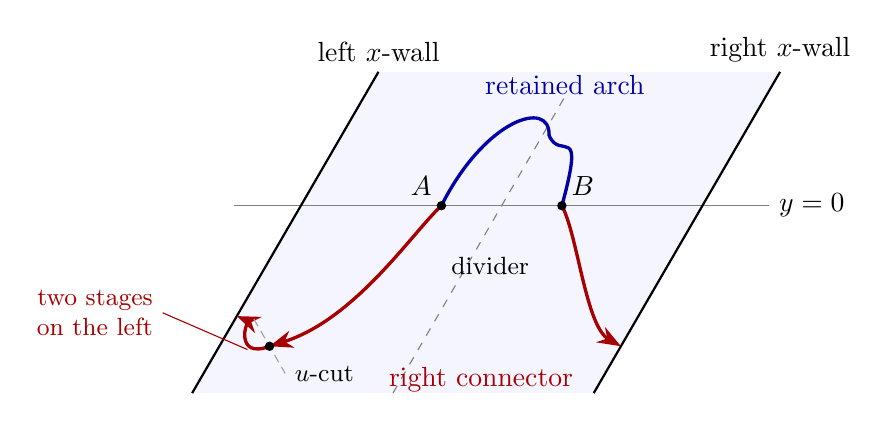
\begin{tikzpicture}[x={(1cm,0cm)},y={(0.58cm,1cm)},scale=.85,>=Stealth]
 \fill[blue!4] (-3,-2.8)--(-3,2)--(3,2)--(3,-2.8)--cycle;
 \draw[gray] (-4,0)--(4,0) node[right,black] {$y=0$};
 \draw[thick] (-3,-2.8)--(-3,2) node[above] {left $x$-wall};
 \draw[thick] (3,-2.8)--(3,2) node[above] {right $x$-wall};
 \draw[dashed,gray] (0,-2.8)--(0,1.6);
 \node[black,font=\small] at (.35,-.9) {divider};
 \draw[very thick,blue!65!black] (-.9,0) .. controls(-1,1.3) and(-.2,1.6) .. (.1,1.05)
 .. controls (.5,.65) and(.5,1.3) .. (.9,0);
 \draw[very thick,red!65!black,->] (-.9,0) ..controls(-1.1,-.4) and(-1.2,-1.7)..(-2.25,-2.1);
 \draw[very thick,red!65!black,->] (-2.25,-2.1)..controls(-2.65,-2.3) and(-2.85,-1.7)..(-3,-1.65);
 \draw[very thick,red!65!black,->] (.9,0)..controls(1.4,-.45) and(2.3,-1.8)..(3,-2.1);
 \fill(-.9,0)circle(2pt)node[above left]{$A$};
 \fill(.9,0)circle(2pt)node[above right]{$B$};
 \draw[densely dashed,gray!75] (-2.72,-1.693)--(-1.78,-2.507) node[right,black,font=\small] {$u$-cut};
 \fill(-2.25,-2.1)circle(2pt);
 \node[blue!65!black] at (-.1,1.8){retained arch};
 \node[red!65!black,align=center] at (1.2,-2.6){right connector};
 \node[red!65!black,align=right,font=\small] (leftlabel) at (-5.15,-1.6){two stages\\on the left};
 \draw[red!65!black,thin] (leftlabel.east)--(-2.55,-2.15);
\end{tikzpicture}

\caption{Schematic two-connector construction. The blue arch is retained,
while the red paths join its ends to opposite $x$-walls. The picture shows
confinement regions and the order of construction, not the microscopic
shape of a typical path. The dashed $u$-cut separates the two stages of the left connector
and makes their split recoverable.}\label{L:fig:connectors}
\end{figure}


\medskip\noindent\textbf{Recovery and the mass balance.}
Both connectors stay below the arch and on their respective sides of
the divider. Their union with the arch is therefore a strict $x$-bridge
of height $R$ and diameter at most $C_0R$, where $C_0$ is fixed.
Translate its left endpoint to the prescribed starting port. Count the input arch, the placement $D$,
and the two connector paths as labels on the resulting bridge. The
construction counts distinct connector paths by the first-cut argument;
internal growth stages are not extra labels.
If $W_R$ denotes this labelled output mass, multiplicativity at ports
and the order $R$ choices of $D$ give
\begin{equation}
 W_R\ge cR\bigl(R^{-1/4}(\log h)^{-C}\bigr)^2a_h
       \ge cR^{1/2}(\log h)^{-C}a_h.
 \label{L:eq:connector-labelled-mass}
\end{equation}

We next recover these labels from the bridge. For any strict $x$-bridge
$\omega$, let $M(\omega)$ be the number of $y$-grid lines above both
endpoints that meet $\omega$ at exactly two crossing ports. In every
constructed output the translated line $y=0$ is one of these lines:
the arch lies strictly above it and both connectors lie strictly below.
Choose this line in an output. Its two crossings determine the subarc
above the line, hence the input arch and its left and right endpoints
$A,B$. Translating $A$ back to the prescribed arch source fixes the
original placement. In particular the gap $g$ and the distance $D$
from $A$ to the left $x$-wall are determined; $R$ is already the output
height. The two remaining subarcs determine the connector paths.

The split of the left connector is also recoverable. The data $R,D,g$
specify its terminal $u$-bin and all the prefix tests used to extract
the direction-change cut. The second part stays strictly beyond that
cut in $u$, so it changes neither the earlier crossing counts nor the
prefix tests. The first qualifying cut on the completed connector is
therefore the cut selected in the construction. Here the first part
is counted as a distinct extracted prefix: its former terminal target
$S$ and the growth stages used before extraction are not retained as
labels. For the second part, its starting port and exact target wall
are now known, so its stage cuts are recovered by the same rule.
Thus each choice of the $y$-line determines at most a fixed number of
input labels, allowing for the finitely many orientation conventions.
The inverse multiplicity is at most $C M(\omega)$.

We need a bound on large values of $M$ that is uniform in the order of
the moment. Let $\mathcal G_R$ be all strict $x$-bridges from the fixed
source, of height $R$ and diameter at most $C_0R$. For
$1\le k\le c_0R$, with $c_0>0$ fixed, we claim
\begin{equation}
 \sum_{\omega\in\mathcal G_R}\mu(\omega)
       \binom{M(\omega)}{k}
 \le C^kR^2\left(C\sqrt{R/k}\right)^{k-1},
 \label{L:eq:double-cut-factorial}
\end{equation}
where $C$ is independent of $k$ and $R$.
To prove this, list the selected levels in increasing order,
$t_1<\cdots<t_k$. There are $O(R)$ choices for the far endpoint and
$O(R)$ choices for $t_1$. The two initial arms, from the two endpoints
to $t_1$, lie below that level between the $x$-walls. Each has bounded
total mass by the convex boundary-flux estimate; a further lower wall
can be placed beyond the diameter bound. Drop mutual avoidance between
these arms for the upper bound.

Between $t_i$ and $t_{i+1}$, connectivity and the two-crossing condition
give two strict $y$-bridges. If $j_i=t_{i+1}-t_i$, their total mass is
at most $B_{j_i}^2\le Cj_i^{-1/2}$. The remaining top arc has bounded
mass by the half-plane arch identity. The positive gaps satisfy
$\sum_i j_i\le C_1R$, for a fixed $C_1$ allowing for the level units.
With $a=k/R$, exponential weighting gives
\[
 \begin{aligned}
 \sum_{\substack{j_1,\ldots,j_{k-1}\ge1\\
                  \sum_i j_i\le C_1R}}
       \prod_{i=1}^{k-1}j_i^{-1/2}
 &\le e^{C_1k}
       \left(\sum_{j\ge1}j^{-1/2}e^{-kj/R}\right)^{k-1}\\
 &\le e^{C_1k}\left(C\sqrt{R/k}\right)^{k-1}.
 \end{aligned}
\]
This proves \eqref{L:eq:double-cut-factorial}, including $k=1$ with
the empty-product convention. Counting the selected levels in
increasing order is what gives $\binom Mk$.

Set $T_R=\sqrt R\log R$. Since $M(\omega)\le CR$ on
$\mathcal G_R$, for $1\le k\le T_R/2$ the preceding estimate yields
\[
 \begin{aligned}
 \sum_{\substack{\omega\in\mathcal G_R\\M(\omega)>T_R}}
       \mu(\omega)M(\omega)
 &\le \frac{CR}{\binom{\lfloor T_R\rfloor}{k}}
       \sum_{\omega\in\mathcal G_R}\mu(\omega)
       \binom{M(\omega)}{k}\\
 &\le CR^{5/2}\sqrt k
       \left(\frac{C\sqrt k}{\log R}\right)^k.
 \end{aligned}
\]
Choose $k=\lfloor c(\log R)^2\rfloor$, with $c>0$ sufficiently
small. For large $R$ this lies in both required ranges, and the last
bound is smaller than every fixed inverse power of $R$. The labelled
mass of constructed outputs with $M>T_R$ is at most a constant times
this bound, so it is negligible compared with
\eqref{L:eq:connector-labelled-mass}. On the remaining outputs the
inverse multiplicity is at most $CT_R$. Hence their unlabelled mass
is at least
\[
 \frac{cR\bigl(R^{-1/4}(\log h)^{-C}\bigr)^2a_h}
      {\sqrt R\log R}
 \ge h^{-1/4}(\log h)^{-C},
\]
after changing $C$, since $R\in[R_0,2R_0]$. This is the required
mass lower bound at each such height $R$.

The connector lengths are at most $CR^{4/3}$, uniformly over the
placements.  Since $R\le2h(\log h)^{1/64}$, their combined length is
at most $C'h^{4/3}(\log h)^{1/48}<\ell_+$ for sufficiently large $h$.
The retained arch has length between $\ell_-$ and $\ell_+$, so every
output counted above lies in $[\ell_-,2\ell_+]$.  Summing the per-height
mass over $R\in[R_0,2R_0]$ and rotating back to the fixed bridge
orientation gives
\begin{equation}
 \sum_{1\le H\le2R_0}
 \mu\{\omega\in\mathcal B_H:\ell_-\le|\omega|\le2\ell_+\}
 \ge c h^{3/4}(\log h)^{-C}.
 \label{L:eq11}
\end{equation}
The earlier bridge alternative obeys the same estimate because
$[h,2h]\subset[1,2R_0]$.  This proves the theorem.
\end{proof}

\begin{proof}[Completion of Theorem~\ref{L:thm:finite}]
Section~\ref{L:part6} proves the bridge mass estimate. The cap construction
in Section~\ref{L:part10} proves the arch lower bound with a fixed diameter
cutoff, and the gap comparison there proves the matching upper bound. Transverse confinement is the second tightness
consequence in Section~\ref{L:part10}; its first moment is
Proposition~\ref{L:prop:box-moment}. Section~\ref{L:step18} proves the
strip diameter tail. The polygon assertion is \eqref{L:eq10}, proved at
the end of Section~\ref{L:part9}.
\end{proof}

\begin{thebibliography}{99}
\bibitem{BeatonEtAl2014}
N.~R.~Beaton, M.~Bousquet-M\'elou, J.~de Gier, H.~Duminil-Copin and A.~J.~Guttmann.
The critical fugacity for surface adsorption of self-avoiding walks on the
honeycomb lattice is $1+\sqrt2$.
\emph{Communications in Mathematical Physics} \textbf{326} (2014), 727--754.
\href{https://doi.org/10.1007/s00220-014-1896-1}{doi:10.1007/s00220-014-1896-1}.
Numbered locators refer to \href{https://arxiv.org/abs/1109.0358v5}{arXiv:1109.0358v5}.

\bibitem{DuminilCopinSmirnov2012}
H.~Duminil-Copin and S.~Smirnov.
The connective constant of the honeycomb lattice equals $\sqrt{2+\sqrt2}$.
\emph{Annals of Mathematics} \textbf{175} (2012), 1653--1665.
\href{https://doi.org/10.4007/annals.2012.175.3.14}{doi:10.4007/annals.2012.175.3.14}.

\bibitem{Frenkel1985}
I.~B.~Frenkel.
Representations of Kac--Moody algebras and dual resonance models.
In \emph{Applications of Group Theory in Physics and Mathematical Physics}
(Chicago, 1982), Lectures in Applied Mathematics \textbf{21}, American
Mathematical Society, Providence, RI, 1985, 325--353.

\bibitem{Glazman2015}
A.~Glazman.
Connective constant for a weighted self-avoiding walk on $\mathbb Z^2$.
\emph{Electronic Communications in Probability} \textbf{20} (2015), no.~86, 1--13.
\href{https://doi.org/10.1214/ECP.v20-3844}{doi:10.1214/ECP.v20-3844}.
\href{https://arxiv.org/abs/1402.5376v2}{arXiv:1402.5376v2}.

\bibitem{GlazmanManolescu2017}
A.~Glazman and I.~Manolescu.
Self-avoiding walk on $\mathbb Z^2$ with Yang--Baxter weights:
universality of critical fugacity and 2-point function.
\emph{Annales de l'Institut Henri Poincar\'e, Probabilit\'es et Statistiques}
\textbf{56} (2020), 2281--2300.
\href{https://doi.org/10.1214/19-AIHP1024}{doi:10.1214/19-AIHP1024}.
Numbered locators refer to \href{https://arxiv.org/abs/1708.00395v3}{arXiv:1708.00395v3}.

\bibitem{HammersleyWelsh1962}
J.~M.~Hammersley and D.~J.~A.~Welsh.
Further results on the rate of convergence to the connective constant of
the hypercubical lattice.
\emph{Quarterly Journal of Mathematics} \textbf{13} (1962), 108--110.
\href{https://doi.org/10.1093/qmath/13.1.108}{doi:10.1093/qmath/13.1.108}.

\bibitem{IkhlefCardy2009}
Y.~Ikhlef and J.~Cardy.
Discretely holomorphic parafermions and integrable loop models.
\emph{Journal of Physics A: Mathematical and Theoretical} \textbf{42}
(2009), 102001.
\href{https://doi.org/10.1088/1751-8113/42/10/102001}{doi:10.1088/1751-8113/42/10/102001}.

\bibitem{Kesten1963}
H.~Kesten.
On the number of self-avoiding walks.
\emph{Journal of Mathematical Physics} \textbf{4} (1963), 960--969.
\href{https://doi.org/10.1063/1.1704022}{doi:10.1063/1.1704022}.

\bibitem{KrachunPanagiotis2026}
D.~Krachun and C.~Panagiotis.
Quantitative sub-ballisticity of self-avoiding walk on the hexagonal lattice.
\emph{Annals of Probability} \textbf{54} (2026), 1109--1125.
\href{https://doi.org/10.1214/24-AOP1730}{doi:10.1214/24-AOP1730}.
Numbered locators refer to \href{https://arxiv.org/abs/2310.17299v1}{arXiv:2310.17299v1}.

\bibitem{LawlerSchrammWerner2004}
G.~F.~Lawler, O.~Schramm and W.~Werner.
On the scaling limit of planar self-avoiding walk.
In \emph{Fractal geometry and applications: a jubilee of Beno\^it Mandelbrot,
Part~2}, Proceedings of Symposia in Pure Mathematics \textbf{72},
American Mathematical Society, Providence, RI, 2004, 339--364.
Section locators refer to
\href{https://arxiv.org/abs/math/0204277v2}{arXiv:math/0204277v2}.

\bibitem{MadrasSlade1993}
N.~Madras and G.~Slade.
\emph{The Self-Avoiding Walk}.
Birkh\"auser, Boston, 1993.

\bibitem{Nienhuis1982}
B.~Nienhuis.
Exact critical point and critical exponents of $O(n)$ models in two dimensions.
\emph{Physical Review Letters} \textbf{49} (1982), 1062--1065.
\href{https://doi.org/10.1103/PhysRevLett.49.1062}{doi:10.1103/PhysRevLett.49.1062}.

\bibitem{Schoenberg1947}
I.~J.~Schoenberg.
On totally positive functions, Laplace integrals and entire functions
of the Laguerre--P\'olya--Schur type.
\emph{Proceedings of the National Academy of Sciences of the United States
of America} \textbf{33} (1947), 11--17.
\href{https://doi.org/10.1073/pnas.33.1.11}{doi:10.1073/pnas.33.1.11}.

\bibitem{ScottSokal2005}
A.~D.~Scott and A.~D.~Sokal.
The repulsive lattice gas, the independent-set polynomial, and the
Lov\'asz local lemma.
\emph{Journal of Statistical Physics} \textbf{118} (2005), 1151--1261.
\href{https://doi.org/10.1007/s10955-004-2055-4}{doi:10.1007/s10955-004-2055-4}.
Locators refer to the
\href{https://people.maths.ox.ac.uk/~scott/Papers/lovasz.pdf}{author version
revised September 28, 2004}.

\bibitem{ZhouBatchelor1997}
Y.~K.~Zhou and M.~T.~Batchelor.
Critical behaviour of the dilute $O(n)$, Izergin--Korepin and dilute
$A_L$ face models: Bulk properties.
\emph{Nuclear Physics B} \textbf{485} (1997), 646--664.
\href{https://doi.org/10.1016/S0550-3213(96)00654-2}{doi:10.1016/S0550-3213(96)00654-2}.
\href{https://arxiv.org/abs/cond-mat/9611156}{arXiv:cond-mat/9611156}.

\end{thebibliography}
\end{document}
